%\documentclass[xelatex,a4paper]{bxjsarticle}
\documentclass[12pt,a4j]{bxjsreport}
%\documentclass[xelatex,a4paper,precisetext,noautoxspacing]{bxjsbook}
%
\usepackage{fontspec}
\usepackage{zxjatype}
\usepackage{titlesec}
\usepackage{xltxtra}
\setjamainfont{ipam.ttf}
\setjasansfont{ipag.ttf}
\setjamonofont{ipag.ttf}


\usepackage{amsmath,amssymb,amsfonts}
\usepackage{bm}
\usepackage{siunitx}
\usepackage{graphicx}
\usepackage{multirow} 
\usepackage[subrefformat=parens]{subcaption}
%\usepackage{mediabb}

\PassOptionsToPackage{hyphens}{url}
\usepackage[dvipdfmx]{hyperref}
\hypersetup{%
 setpagesize=false,%
 bookmarks=true,%
 bookmarksdepth=tocdepth,%
 bookmarksnumbered=true,%
 colorlinks=false,%
 pdftitle={},%
 pdfsubject={},%
 pdfauthor={},%
 pdfkeywords={}}
%\captionsetup{compatibility=false}
%\usepackage[top=-5truemm,bottom=25truemm,left=20truemm,right=20truemm]{geometry}

\titleformat*{\section}{\LARGE\bfseries\sffamily}
\titleformat*{\subsection}{\Large\bfseries\sffamily}
\titleformat*{\subsubsection}{\large\bfseries\sffamily}

%\usepackage[colorlinks=true, bookmarks=true,
%bookmarksnumbered=true, bookmarkstype=toc, linkcolor=blue,
%urlcolor=blue, citecolor=blue]{hyperref}
\setcounter{secnumdepth}{4}


\title{インタラクティブ遺伝的アルゴリズムを用いた\\
プロシージャルモデリング支援システムの提案}
\author{細川 岳大}
\date{2024年1月18日}

\begin{document}

\thispagestyle{empty}
\begin{center}
 修士論文\\% どちらか一方を消してください.
\vfill
インタラクティブ遺伝的アルゴリズムを用いた\\
プロシージャルモデリング支援システムの提案\\
\vfill
細川 岳大\\
\vfill
主指導教員\ \ 宮田\ 一乘\\
\vfill
北陸先端科学技術大学院大学\\
先端科学技術研究科\\
(知識科学)\\ %取得希望学位
\vfill
令和6年3月\\ % 学位授与年月
\vfill
\end{center}
\clearpage

\newpage

\centerline{\scalebox{1.5}{\textbf{Abstract}}}
\vspace{12pt}



In recent years, with the advancement of 3D computer graphics content, there is a growing demand for high-quality and abundant content. Consequently, procedural modeling, which allows shape editing through parameters, has been widely employed. However, the increase in the number of parameters for improved quality poses a challenge, leading to a concern about extended development time. 


To address this issue, this study proposes a modeling support system that combines model proposals using interactive genetic algorithms and interpolation through a two-dimentional user interface (UI). We utilize genetic algorithms for their versatility and expand the exploration range through an enhanced UI compared to conventional approaches. 


The proposed system performs exploration through three types of operations.
First, select three from six recommendation models. This reduces the burden on decision-making compared to traditional interactive genetic algorithms by providing fewer choices.Subsequently, interpolation is conducted by dragging a pointer on a two-dimensional UI. The interpolation operation enables exploration of areas beyond the recommendation models. Therefore, it can compensate for the reduced exploration space resulting from the fewer choices.Finally, a slight adjustment of parameters is performed as conventionally done. Since there are constraints on the interpolation operation within the search space, fine-tuning allows for a better reflection of the user's intentions. After these operations, new recommendation models are computed using genetic algorithms. This sequence of steps is repeated to assist users in modeling.


While the experiment and survey results confirm the usefulness of the UI, the effectiveness of genetic algorithms could not be conclusively established. Furthermore, the proposed system is expected to demonstrate its effectiveness when dealing with a large number of parameters during free-form modeling.


A future challenge involves refining the model proposal method and exploring its application to other procedural content generation techniques.

%% 目次
\tableofcontents
\listoffigures
\listoftables

%%%%%%%%%%%%%%%%%%%%%%%%%%%%%%%%%%%%%%%%%%%%%%%%
%%%  本文
%%%%%%%%%%%%%%%%%%%%%%%%%%%%%%%%%%%%%%%%%%%%%%%
\newpage 
\setcounter{page}{1}

\chapter{序論}

\section{研究背景}
近年ハードやソフトの技術進歩により, 3 Dimensional Computer Graphics(3DCG)の表現力が向上している.特にゲームやメタバースなどの開発においては詳細な表現から広大なマップまで,高いクオリティが求められることも多くなっている.そのため大規模な開発では数年かかることも多くなっている.そこで, 3DCG 開発においてプロシージャルモデリングという手法がよく利用されている.プロシージャルモデリングとは,数式などの処理を組み合わせてモデリングを行う手法であり,計算処理を設計後は,あらかじめ設定された複数の説明変数のパラメータを変更するだけで様々なモデルを生成する事が出来る手法である.開発者以外がプロシージャルモデリングに触れる機会として,ゲームのキャラクタークリエイトが挙げられる.身長や体格,顔の位置といった様々な値を変更することでプレイヤーの好きなキャラクターを作成する事が出来る.図\ref{fig:metahuman_cc1}に MetaHuman\footnote{\url{https://www.unrealengine.com/en-US/metahuman}}によるキャラクタークリエイトを示す.一方で前述の通り表現力の向上から,操作するパラメータの個数が増えてきていることはキャラクタークリエイトにおける調整を行う事が出来るパラメータ数の向上具合から見ても明らかである.図\ref{fig:blenderSFT}に Blender\footnote{\url{https://www.blender.org/}} によるプロシージャルモデリングの様子を示す.画像右側に並んでいるのが操作する事が出来るパラメータであり,このモデルではおよそ30個存在するため,画面上に収まっていない.パラメータの個数が増えることはその分一つのオブジェクトにかける開発時間の増加を伴う.加えて,コンテンツ自体の内容量が増加しているためモデリングを行うオブジェクトの数も増加傾向にあるので,開発時間の増大が著しい.そこで本研究では,モデリング時間の短縮のために操作するパラメータ数の多さに着目し,パラメータ数の削減によってモデリング時間短縮を試みる. 


複数のパラメータを操作し適したモデリングを行うというのは,開発者の考える最適なパラメータを設定するという点で組み合わせ最適化問題として捉える事が出来る.そこでメタヒューリスティクスで組み合わせ最適化問題に有効な手法としてユーザとの対話が可能なインタラクティブ遺伝的アルゴリズムを用いてモデル提案を行うことで効率的な探索を行えることを期待する.


\begin{figure}[h]
	\begin{center}
		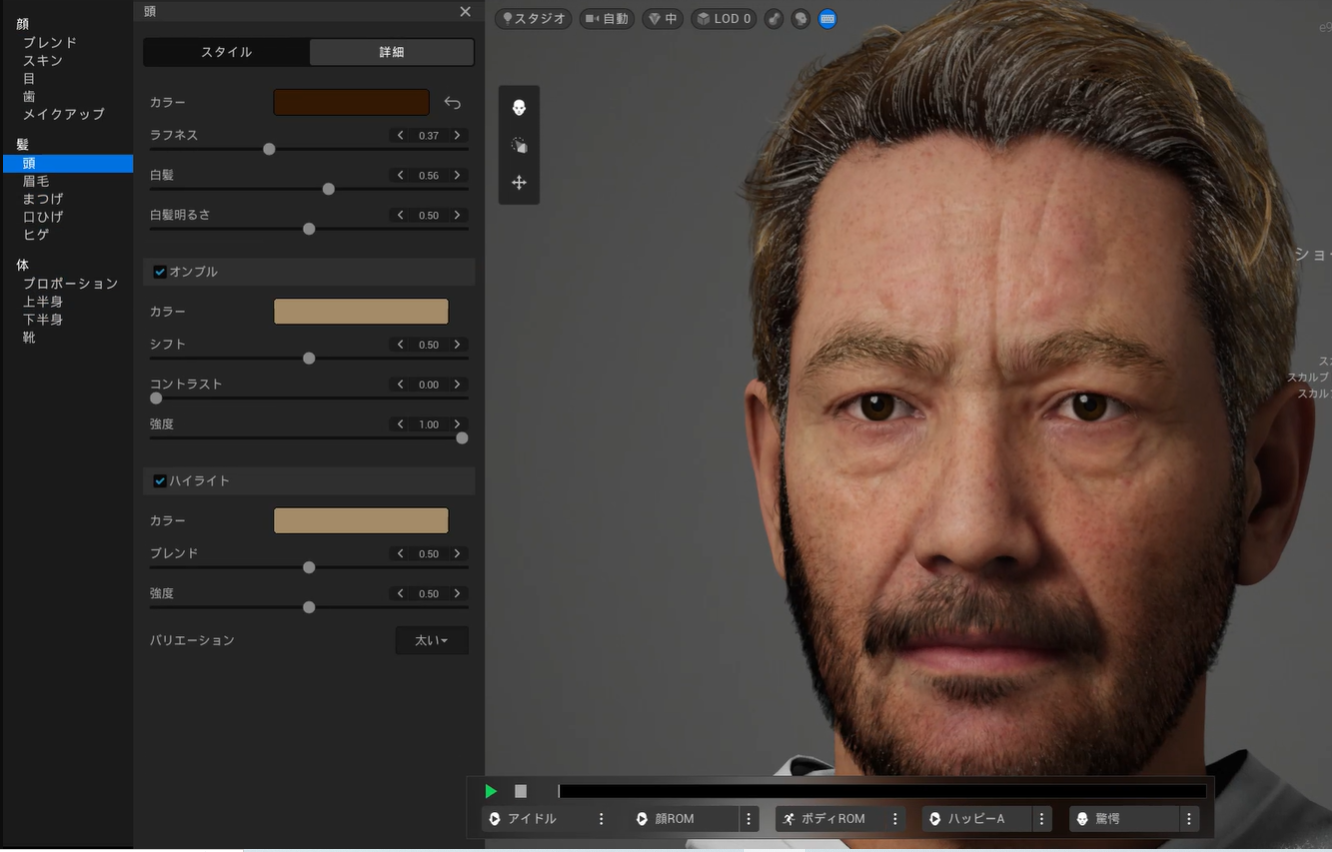
\includegraphics[scale=0.4]{./imgs/metahuman1.PNG}
		\caption[MetaHuman におけるキャラクター作成]{MetaHuman \hyperref[fn:3]{\footnotemark[3]}におけるキャラクター作成\label{fig:metahuman_cc1}}
	\end{center}
\end{figure}

\footnotetext[3\label{fn:3}]{\url{https://metahuman.unrealengine.com/}}

\begin{figure}
	\begin{center}
		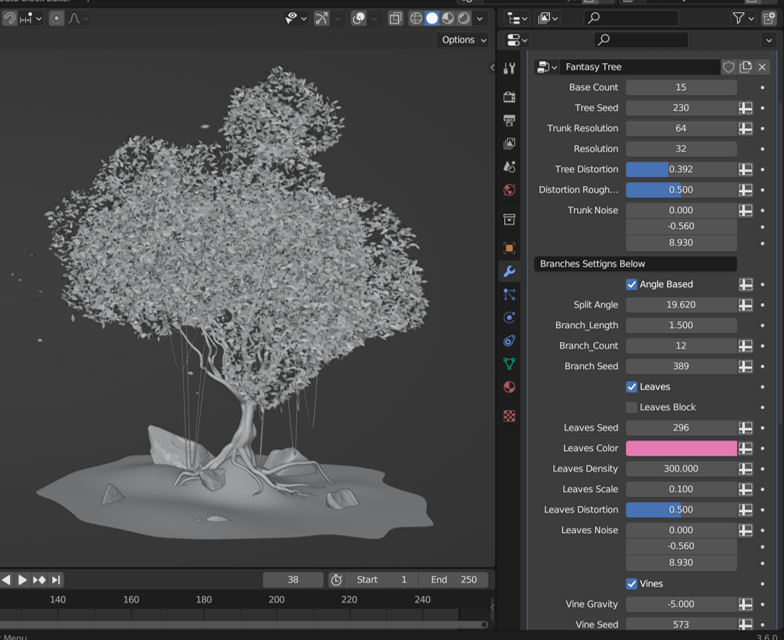
\includegraphics[scale=0.5]{./imgs/blenderSFT.PNG}
		\caption{Blender におけるプロシージャルモデリング\label{fig:blenderSFT}}
	\end{center}
\end{figure}

\newpage
\section{研究目的}
    本研究では,プロシージャルモデリングにおいて制作時間短縮を目的とし,インタラクティブ遺伝的アルゴリズムを利用した操作パラメータ数を削減したシステムを提案し,ユーザ実験を通して検証を行う.操作パラメータ削減によって制作時間短縮だけでなくユーザビリティの向上に繋げることも目的とする.



\section{論文構成}
    本論文は5章で構成する.まず,2章では要素技術および関連研究について紹介する.続いて3章で実験手法の提案をし,4章において実験結果と考察を示す.5章で本研究の成果をまとめた上で,今後の課題について述べる.

\clearpage

\newpage

\chapter{関連技術}
本章ではプロシージャルモデリングおよび遺伝的アルゴリズムについての詳細および関連研究について紹介する.

\section{プロシージャルモデリング}
\subsection{概要}
\ プロシージャルモデリングとは,研究背景にも簡単に記載した通り,数式などの計算処理を組み合わせてモデリングを行う手法である. CG 分野で非常に幅広く活躍している技術であり,単なるオブジェクトだけでなく,計算機の能力にもよるがエフェクトや物理演算といったリアルタイムでの変化が必要なものに対しても用いられている.近年ゲーム業界では,オープンワールドのような広大なマップを作成するのにあたり,特に注目を集めている.

\subsection{関連研究}\label{label:relatedResearch}
プロシージャルモデリングについての研究として,大きく3つに分かれている.


一つ目は,植物\cite{lintermann1999interactive}や地形\cite{smelik2011declarative}といった自然物から城\cite{三浦嘉大2020地理的要素とユーザー自由度を考慮した日本城郭都市のプロシージャルモデリング}やビル\cite{muller2006procedural}などの人工物,煙\cite{xie2022dualsmoke}や火などの一つの状態を持たないパーティクルなど物体表現に焦点を当てた研究である.特に近年物体表現に焦点をあてたものに関して Sketch-base による形状指定することでの生成研究は多い反面,パラメータを手作業で調整するものの研究は数が少ない.その理由としては,研究背景の説明にもある通り,表現をより良くすることによるパラメータ数増大が原因であると考えられる.


次は機械学習と組み合せた研究\cite{DBLP:journals/corr/abs-2010-04548}である.特にこの研究は近年非常に目覚ましい成果を挙げており,その中でも特に顕著なものはゲームにおけるレベルデザインに関する研究である.理由として,モデリングに関する評価を自動テストによってどの程度の難易度であるかを評価できる点にある.


そして最後に紹介するのが,プロシージャルモデリング時の効率的な作成システムに着目した研究である.


koyama らはベイズ最適化を用いた手法である BO as Assistant \cite{koyama2022bo}を提案している.図\ref{fig:boAssistant1}にシステムの実装画面を示す.
この研究では,プロシージャルモデリングにおけるパラメータ操作以外に,3つの提案モデルがベイズ最適化によって生成され,従来のパラメータ操作に加え,そのモデルに対する補間操作を行う事が出来るスライダーが追加されている.
また生成状況に合わせて再提案のボタンを押す事で別のモデルが提案されていき,プロシージャルモデリングのパラメータ操作を複数同時に行えるため,その分効率的なモデリングが出来たとされている.一方で,ベイズ最適化のモデリングにおけるパラメータ数に制限があるとされている.

図について
, Design preview は操作が行われるモデルであり,各パラメータのスライダーと Blending slider を動かすことで変化する. Blending slider は各 Suggestion モデルとの補間を行う事が出来,一番右端にスライダーを移動させることで, Design preview が対応する Suggestion モデルと一致する. Regenerating button を押すことで,現在の Design preview が獲得関数が最大になる直近のデータとしてベイズ最適化に適用され, 
再計算された獲得関数にサンプリングし Design preview を除いた上位3つが Suggestions として更新される.
本研究ではこの手法との対照実験を行う.

\begin{figure}[h]
	\begin{center}
		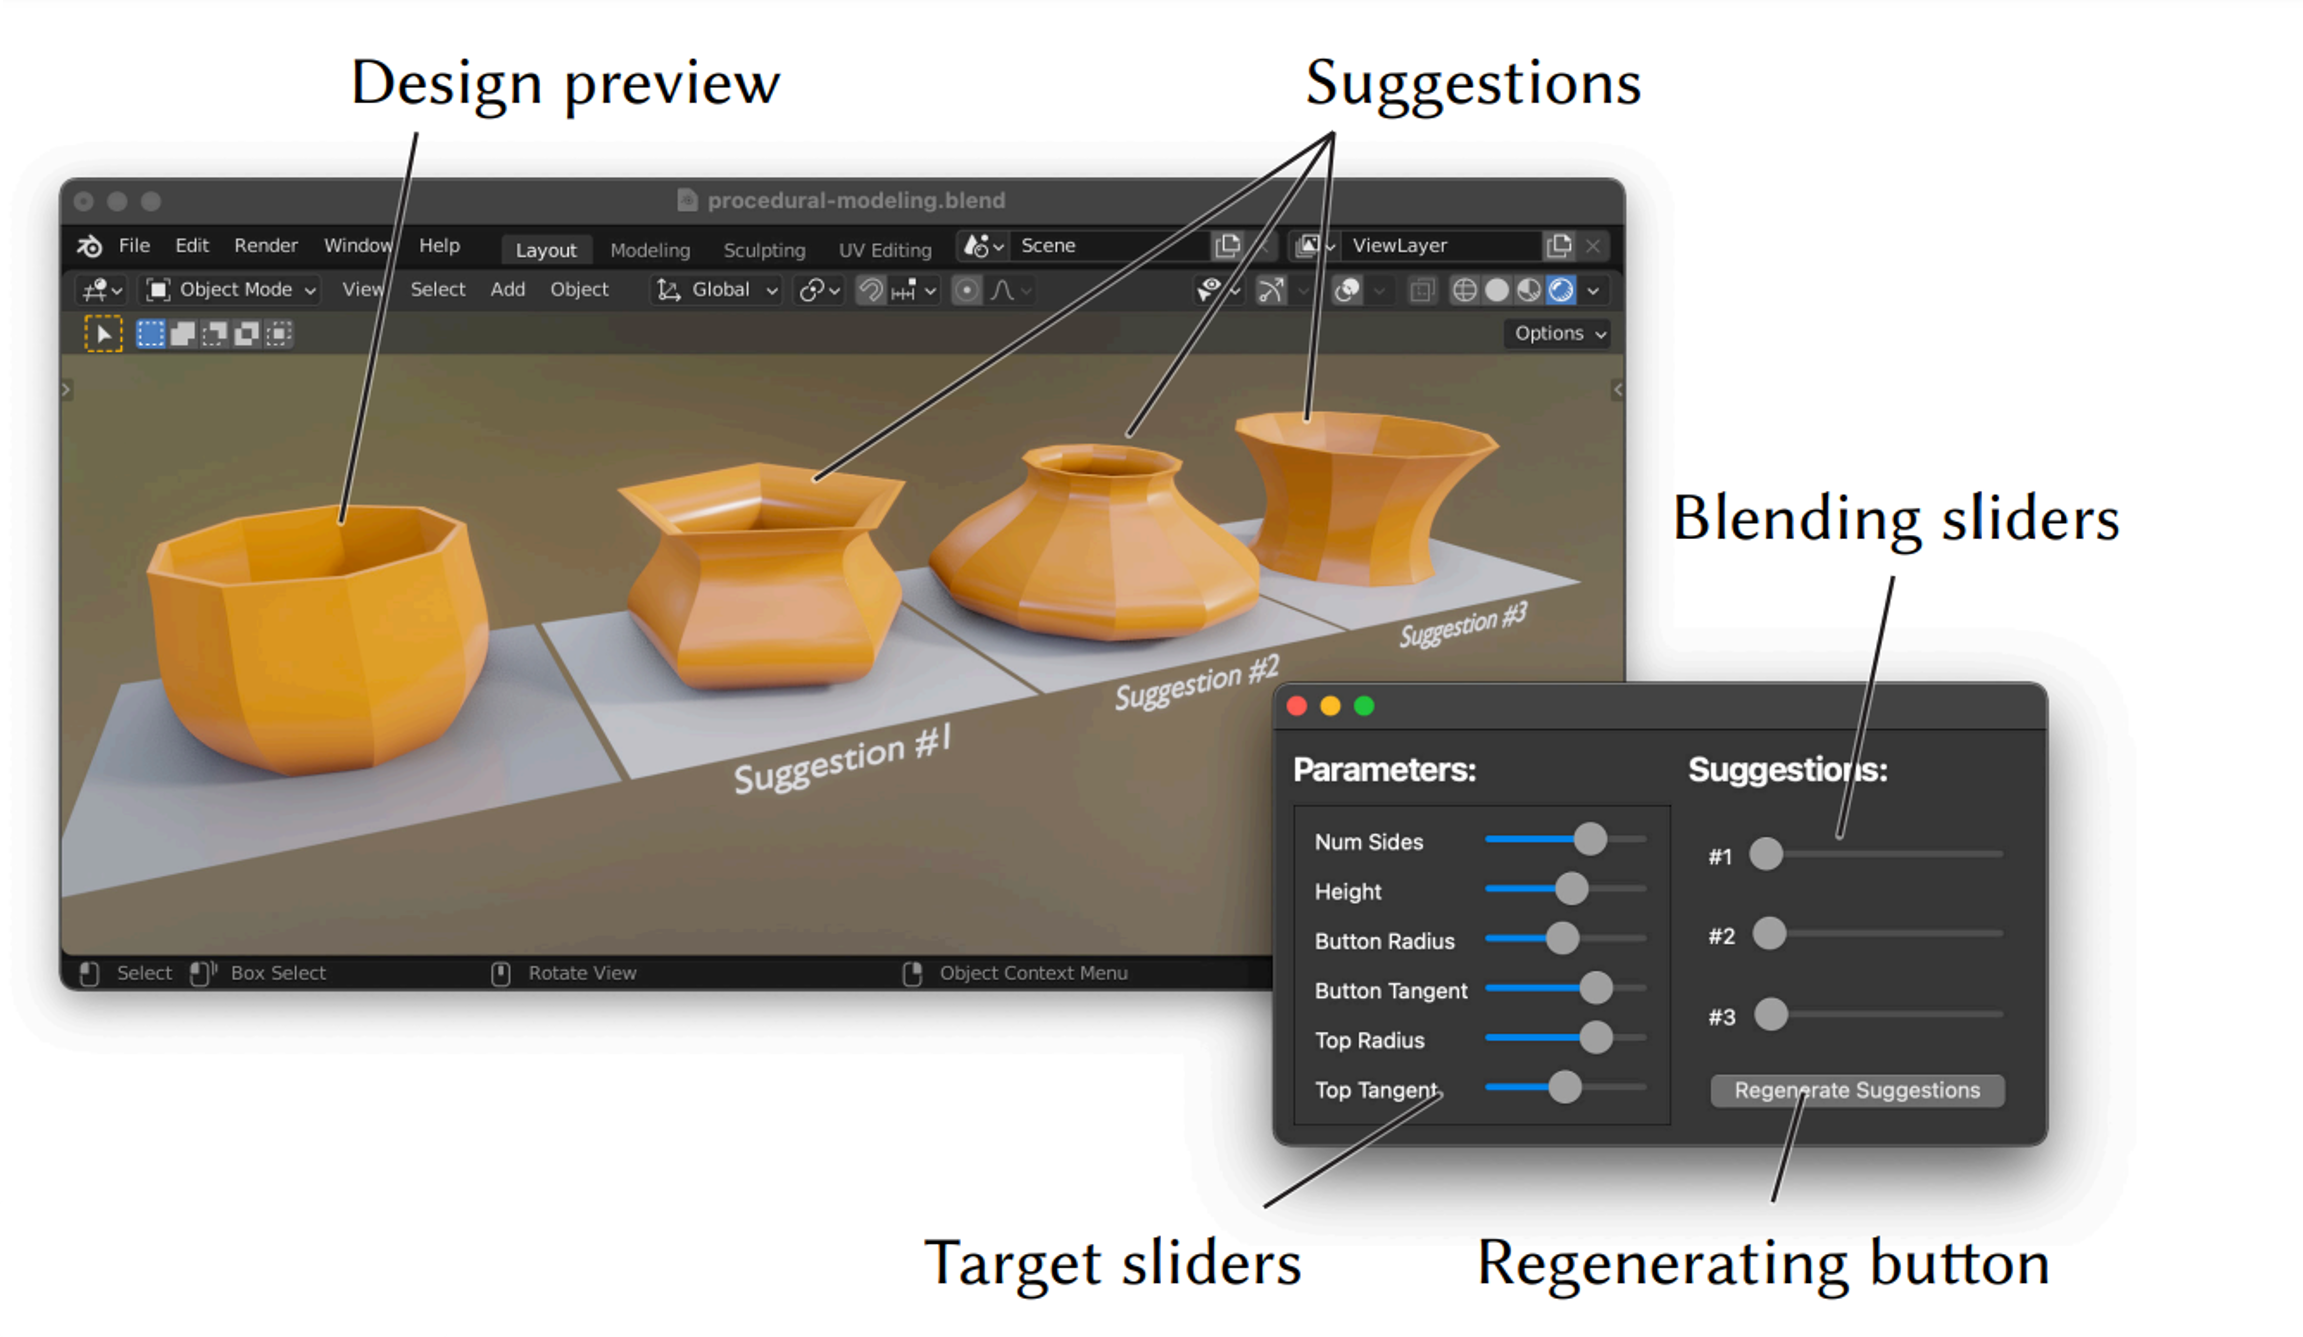
\includegraphics[scale=0.7]{./imgs/boAssistant1.png}
		\caption[BO as Assistant]{BO as Assistant (: 先行研究\cite{koyama2022bo}の Preview Video より引用\label{fig:boAssistant1})}
	\end{center}
\end{figure}


\newpage

\section{インタラクティブ遺伝的アルゴリズム}
  インタラクティブ遺伝的アルゴリズム(Interactive Genetic Algorithm : IGA)とは,ユーザとの対話を用いた遺伝的アルゴリズムである.まず遺伝的アルゴリズムの概要について説明の後,インタラクティブ遺伝的アルゴリズムについての詳しい説明を行う.

\subsection{遺伝的アルゴリズム}
  遺伝的アルゴリズム (Genetic Algorithm : GA)\cite{whitley1994genetic} とは,生物の進化を模倣した組合せ最適化問題のアルゴリズムであり,メタヒューリスティクスとしてよく利用される. 
  
  解の要素の最小単位を遺伝子,遺伝子の集まりである解を個体として表現する.また個体の集合を世代とし,各個体の計算された適応度をもとに選択,交叉,突然変異の3つの操作によって新たな個体群を生成し,次世代の個体集合とする.個体の適応度評価と前述の3操作によって,1世代において適応度の高い遺伝特性を持つ個体が増加する.それによって最適解に近づいてく.
  
  個体の基本的なエンコーディング方法として,バイナリ型,順列型,実数型,整数型がある.本研究では特に実数型について取扱うため,以降実数型を前提とした説明を行う.

\subsubsection{選択}
  選択\cite{blickle1996comparison}は自然淘汰をもとにした操作であり,個体の適応度にもとづき次世代に残される個体を選ぶものである.以下のものがあげられる.

\begin{itemize}
	\setlength{\leftskip}{25mm}
	\item[エリート選択\cite{murata1996multi} : ]世代における適応度の最も高い個体を他の操作を行わず次世代に残す手法である.

	\item[トーナメント選択 : ]個体群からランダムに決められた数(: トーナメントサイズ)取り出し,
	その中で適応度の最も高い個体を選択する手法である.
\end{itemize}


\ これら選択操作によって,適応度の高い個体,つまり世代の中で評価の高い個体の遺伝子が次に引き継がれることによって,前世代において評価の高い遺伝子特性の一部が次世代に引き継がれる.


\subsubsection{交叉}
交叉は生物の交配をもとにした操作であり,2つの個体から新たな2つの個体を生成するものである.遺伝子の種類が有限集合であるバイナリ型や一部の整数型は,生物の遺伝子を模倣した交叉である二個体における遺伝子の交換操作によってなされる交叉が利用できるのに対して,無限集合である実数型は利用できない.遺伝子の交換による交叉だけでは,二つの遺伝子の間に最適となる遺伝子があったとしても探索出来ないので,有限集合における交叉方法では探索が不十分である.そこで,以下のものが挙げられる.
\begin{itemize}
	\setlength{\leftskip}{0mm}
	\item Blend Clossover alpha (BLX-$\alpha$) : 
        \begin{enumerate}\setlength{\leftskip}{5mm}
            \item[] 2つの親個体からなる区間の両端$\alpha$倍した領域においてランダムな子個体を生成する.
        \end{enumerate}
        
	\item Unimodel Normal Distribution Crossover (UNDX)\cite{ono1999robust} : 
        \begin{enumerate}\setlength{\leftskip}{5mm}
            \item[] 3つの個体を用いた交叉であり,そのうち二つを直線で結び,残りの個体と直線との距離を広がりに持つような多次元正規分布によって子個体を生成する.
        \end{enumerate}
 
        \item 多親交叉 Real-coded Ensemble Crossover (REX)\cite{小林重信2009実数値} : 
         \begin{enumerate}\setlength{\leftskip}{5mm}
            \item[] 複数の親個体を用いた交叉であり,その親の重心を取ったのち,全ての親に対し任意の確率分布に従う確率変数を重みとして移動させたものを新たな子個体として生成する.UNDXを多親個体として一般化したものに相当する.
        \end{enumerate}
\end{itemize}

\subsubsection{突然変異}
個体の遺伝子を変化させる操作で,局所探索になることを防ぐ.
乱数によって他の取りうる値に変化させる.また,突然変異率を上げすぎるとランダム探索となり,
収束しなくなるため,高くても数\%に設定されることが多い.

\subsection{IGA と GA の違い}
図\ref{fig:iGAOverView}にインタラクティブ遺伝的アルゴリズムの概略図を示す.
インタラクティブ遺伝的アルゴリズムが通常の遺伝的アルゴリズムと違う点は,適応度計算が計算機によって自動で行われるか,ユーザが行うかの違いである.
\begin{figure}[h]
	\begin{center}
		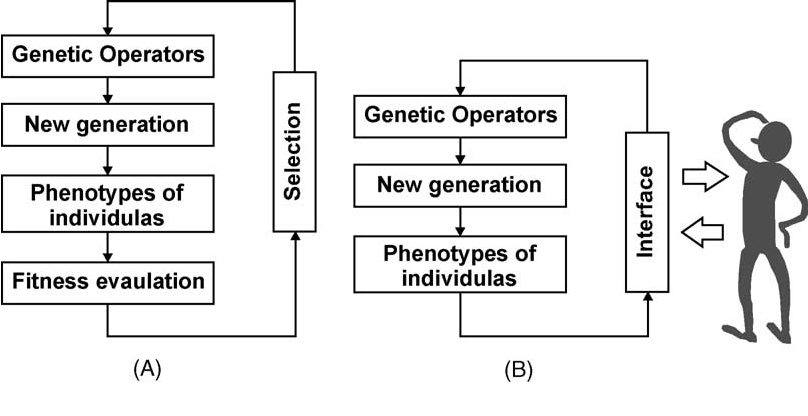
\includegraphics[scale=0.5]{./imgs/iGA_overview2.png}
		\caption[IGA の概略図]{(A) GA の概略図,(B) IGA の概略図 (: 文献\cite{MADAR20051591}の Figure 1より引用\label{fig:iGAOverView})}
	\end{center}
\end{figure}

遺伝的アルゴリズム自体がメタヒューリスティクスであるため,
人間の認識といった計算機では測れないブラックボックスな問題にも適応する事が出来る.しかし問題点として,計算機ほど素早く適応度の計算を行う事が出来ない.適応度計算は基本的に,複数の選択肢を提示しそれに点数をつけたり,あるいはより単純に良いか悪いかを選択するといった方法で行われる.そのため,遺伝的アルゴリズムがより良い近似解を出すのに必要な個体数や世代数が稼ぐ事が出来ないという点も問題となる.


\subsection{関連研究}
インタラクティブ遺伝的アルゴリズムの研究については人間の負担をどのように減らすかが特に重要視されており,近年では機械学習と組み合わせた研究\cite{gypa2023propeller, li2023quantification}も盛んである.


機械学習を用いない研究としては, wang らの研究\cite{wang2020method}では,KJ 法を用いることであらかじめ探索範囲を絞ることで実現している.また,mikiらの研究\cite{miki2006global}では,複数人で分散的に探索を行うことで一人の負担を減らしつつも,個人個人の意見を考慮しつつの探索を可能にしている.また,その他にも様々な製品\cite{dong2008tile, 竹之内宏2022対話型人工蜂コロニーアルゴリズムを用いたランニングシューズデザインシステム}への活用研究もなされている.しかしそれらの研究について,制限としてインタラクティブ遺伝的アルゴリズムに用いられる遺伝子数,つまりパラメータの数は10個前後であることが多い.

\section{本研究の位置づけ}
本研究ではプロシージャルモデリングにおける操作負担を減らすことが目的となる.そのためにいくつかのモデルを提案することで,より効率的なモデリングの手助けをさせる.そのうえで,既存の最適化手法ではパラメータ数に制限がかかる問題があるが,それをインタラクティブ遺伝的アルゴリズムを用いて解決できないかと考えた.そして,パラメータ数の多い場合ではその分探索範囲を広げるために,従来のような複数の選択肢から選ぶ方法だけではなく,複数の選択肢を補間されたものを選択するシステムの手法を考案した.インタラクティブ遺伝的アルゴリズムと補間操作を組み合わせたシステムによってモデルの提案を行うことに新規性を有しており,より多くのパラメータを持つプロシージャルモデリングに対して時間短縮を行えることを期待する.
\clearpage

\newpage

\chapter{提案手法}

  本章では,プロシージャルモデリングにおける操作パラメータを削減したシステムの提案を行う.

\section{システム}
\subsection{システム概要}
図\ref{fig:systemFlow},\ref{fig:systemUI}に提案システムのフロー図およびシステムUI の概略図を示す.また,図\ref{fig:systemAno}に実装したシステムを示す.
図\ref{fig:systemAno}について,


まず操作1では,UI 上の数字のボタンによって番号に対応する提案モデルを3つ選択する.
次に操作2で三角形のUIで赤色のポインタを操作することにより,選択された3つのモデルの補間を行う.この時,ポインタの位置が三角形の頂点に近づくほど,その点に対応するモデルに近づく.
そして操作3は ADJ ボタンを押すことで,各パラメータを個別に調節できるサイドバーを表示することが出来る.それによって従来のプロシージャルモデリングと同じく個別の調整が可能となる.
そして, NEXT ボタンを押すことで提案モデルを変更していく.


以上の操作を何度も繰り返すことで,自身の好きなモデルを生成していく.そして最後に END ボタンによって操作を終了する.また,フロー図上では簡略化のため選択と補間を一方通行に記載しているが,実装上では選択中の数字のボタンを再度押すことで選択を外すことが出来,その後別の数字ボタンを押して補間対象のモデルに別の提案モデルを設定することが出来る.
\clearpage

また図\ref{fig:systemUI}に示すように,前述した操作に加え HIDE ボタンを実装する.これは,操作モデル以外を一時的に非表示,再表示する機能を持つ.補間操作によってモデルのサイズが大きくなり,提案モデルや補間対象のモデルと重なる場合がある.その場合に操作の邪魔になるため,提案するシステム操作に対して新たに組み込んだ.

\begin{figure}[h]
    \centering
  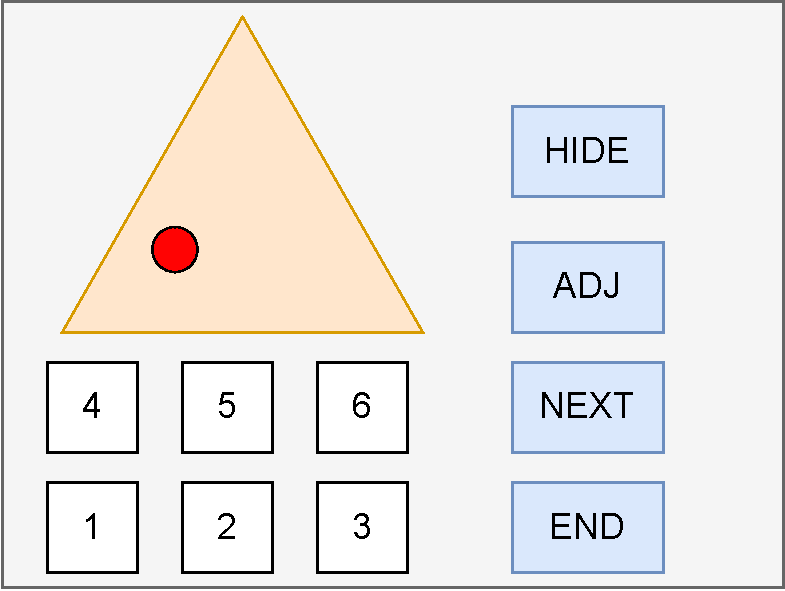
\includegraphics[width=0.55\textwidth]{./imgs/systemUI.pdf}
  \caption{システム UI の概略図}\label{fig:systemUI}
\end{figure}

\begin{figure}[h]
    \centering
  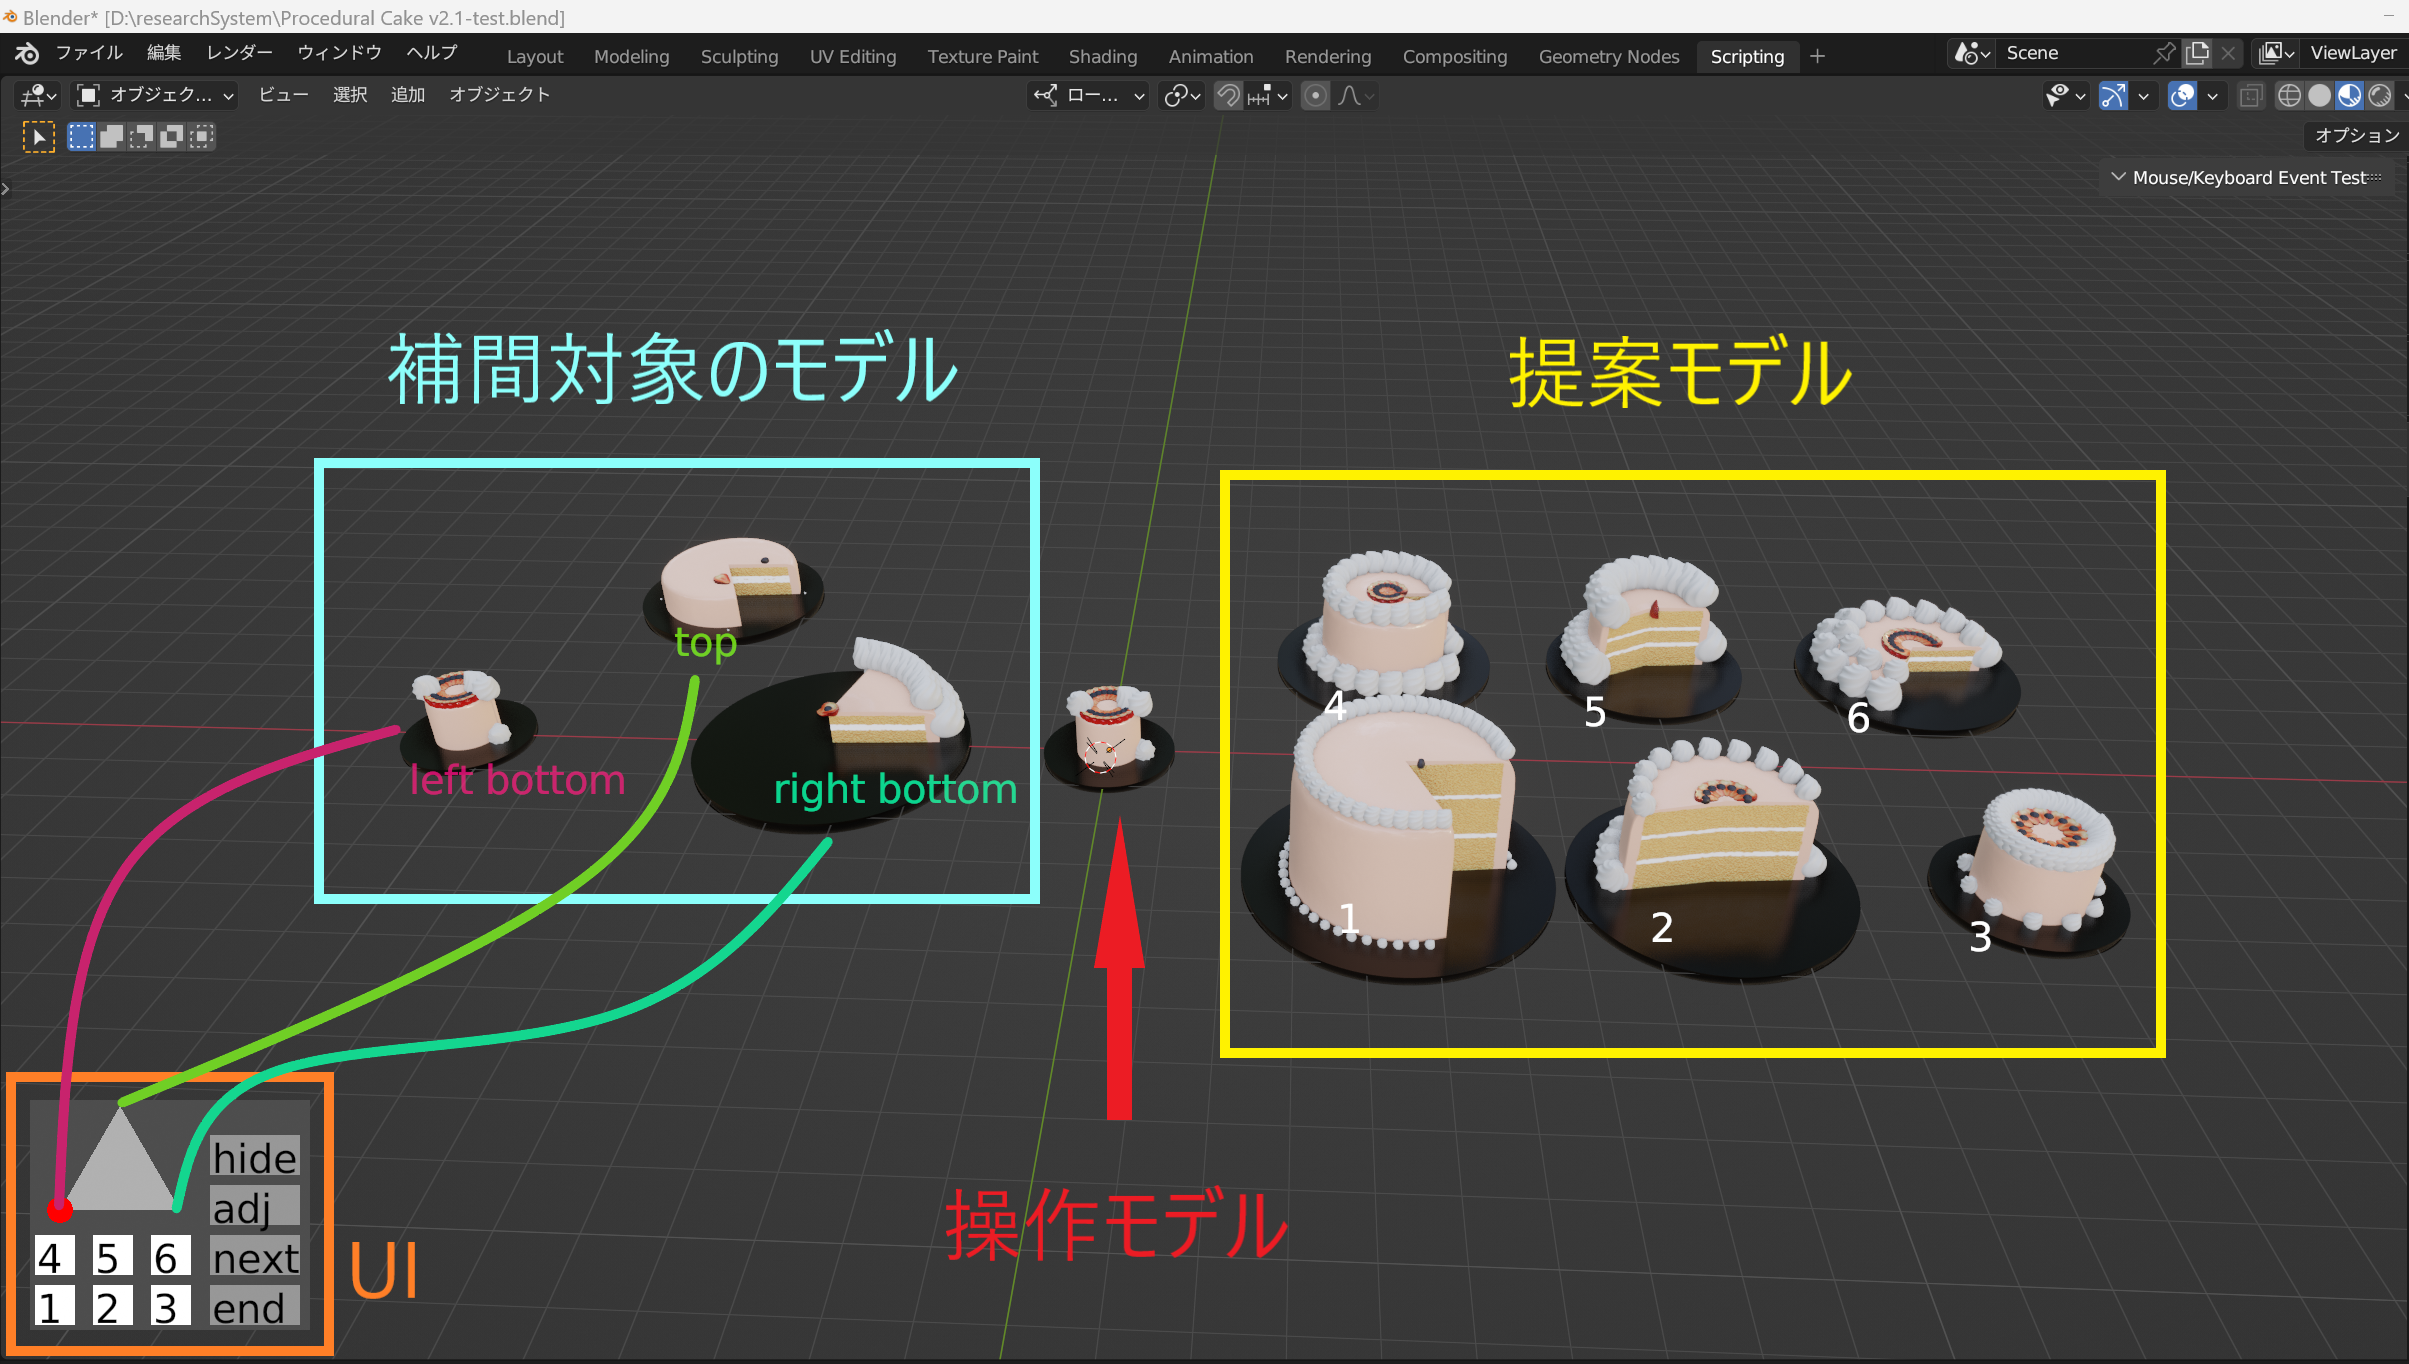
\includegraphics[width=1.0\textwidth]{./imgs/system_ano.png}
  \caption{実装したシステム}\label{fig:systemAno}
\end{figure}

\clearpage
\begin{figure}[h]
    \centering
  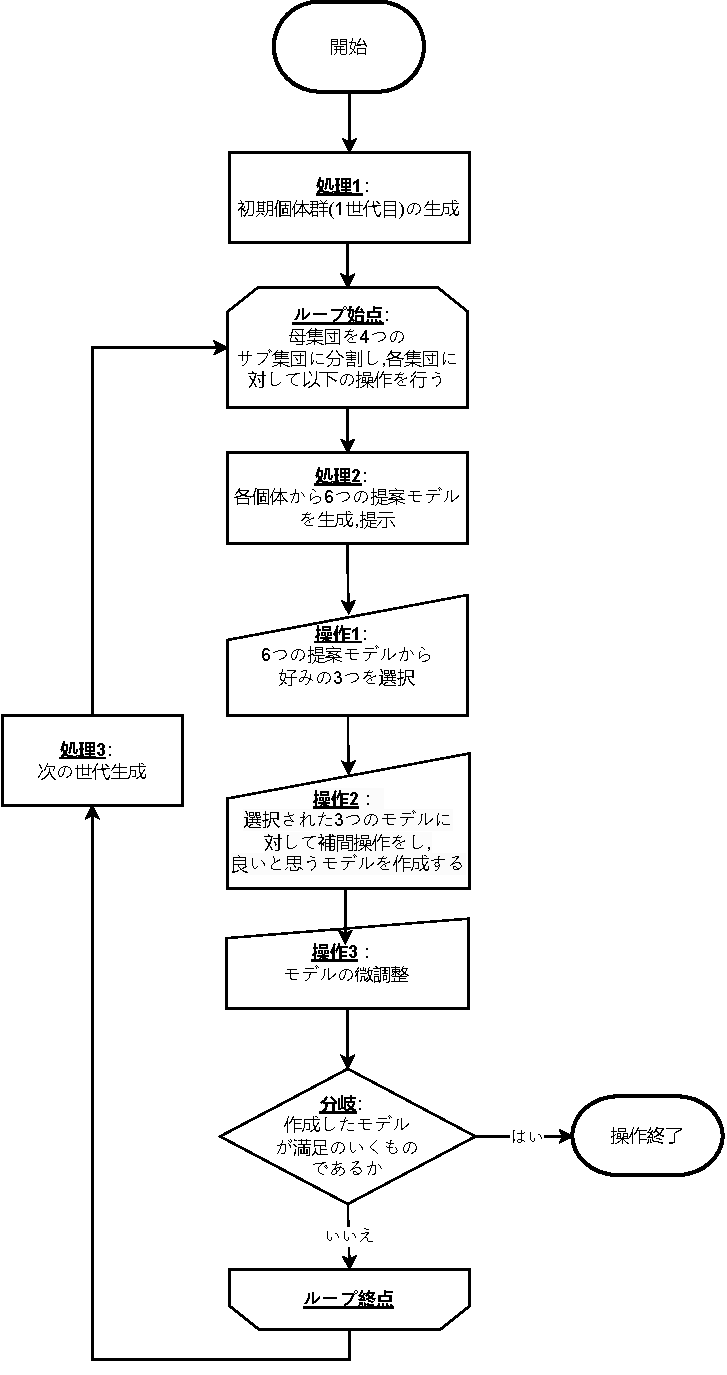
\includegraphics[width=0.7\textwidth]{./imgs/systemFlow.pdf}
  \caption{システムフロー図}\label{fig:systemFlow}
\end{figure}
\clearpage


\subsection{個体表現}
まず,プロシージャルモデリングには様々な入力データが存在する.

\begin{itemize}
      \item 整数値
      \item 実数値
      \item あらかじめ制作された複数のアセット(テクスチャなど)
      \item ストローク
\end{itemize}

提案システムでは,複数の個体を用いたパラメータ補間を行う.そのため,整数値は離散値ではあるため内部的に実数値として処理を行った.式\ref{set:Z},\ref{set:R}が処理を行った前後の集合である.
パラメータ$a$が$[m,n]$の整数値であるとき,$[m,n+1)$の実数値上における同じ値への変換を行い.入力パラメータへの変換は少数以下切り捨てによって行う.

\begin{equation}\label{set:Z}
 \{a | m \leq a \leq n , a\in\mathbb{Z}\}
\end{equation}
\begin{equation}\label{set:R}
 \{a | m \leq a < n + 1 , a\in\mathbb{R}\}
\end{equation}

また,アセットを設定するような入力データについて,補間を行う際にアセットの順序性について検討する必要がある.アセットについても有限個であるため,前述した整数値と同様の処理が内部的に行われ,各整数とアセットとを対応させる.そのため補間が行われるときに常にある順番でアセットが変わることになる.この順序性の検討は本研究の範囲外であるため,今回の実験には含めていない.
さらにストロークによって枝の形状やオブジェクトの配置を指定するようなプロシージャルモデリングの場合,
ストロークに対しては,有限個の頂点情報を結ぶことによって表現されているため,順列コーディングと組み合わせることで表現を行うことはできる.しかし,その表現を補間する手法やそれをシステムUI内で再現することは非常に難解なため,本研究では扱わない.


従って,本研究の遺伝子は全て実数値コーディングとして扱う.また遺伝子長については,実装されたプロシージャルモデリングによって設定されたパラメータによって決定されるため様々であり,本研究では汎用性のあるシステム設計を行うことを考えているため,長さは使用するモデルのパラメータ数に応じた可変長である.

\clearpage
\subsection{システム操作と GA 操作の関係}
提案システムは従来の GA 操作と類似点を持たせるように設計する.これにより1ステップにおける GA 操作を疑似的に増やし,収束速度を速める試みをする.

\subsubsection{選択操作}
複数の選択肢からいくつかを選択するという操作は名前の通りであり,従来の IGA でも同じ操作によって親個体の選択が行われる.ただし,従来のものではより多くの選択肢から選択するが,提案システムでは補間操作を行うことで,選択されたモデル以外のモデルについても閲覧,決定を行う事が出来る.
つまり補間操作を加えた探索範囲は補間対象である3つの個体が存在する平面空間上という制約はあるが,ユーザのドラッグ操作により連続的に行える.
従来の IGA の提案では1ステップでの探索範囲は有限個の提案モデル群のみであり,離散的にしか行えない.
そのため,本システムでは提案モデル数を従来よりも減らしても良いと考える.また,ドラッグ操作の手間はあるものの,選択肢の数を減らすことで一度の意思決定のストレスを減らす事が出来る.

\subsubsection{補間操作}
補間操作はユーザのドラッグ操作によってモデルを連続的に閲覧することが可能であり,
探索された平面空間上においてユーザ評価がより高いモデルを決定する事が出来る.
これは,限定的ではあるが交叉操作に類似している.
図\ref{fig:UNDX}に3つの親個体($\bm{x}1,\bm{x}2,\bm{x}3$)を用いて交叉を行う UNDX の個体生成分布図を示す.この分布は遺伝子数と同じ次元数を持つ多変量正規分布として広がる. UNDX ではこの分布に従って子個体が生成される.ただし, UNDX では正規分布として直線上に子個体が生成されるという点から,変数間の依存性が高いものに強力な一方で広い探索範囲をカバーできない欠点がある.一方で,提案する補間操作では,3つの個体が存在する平面空間という制約上で探索し選択されるという点で類似している.また探索空間を限定する反面,その平面上を隙間なく探索できるためユーザ感性における適応度が最大化した個体を発見する可能性が高いという点では,従来の IGA よりも優位な個体を選別出来ていると考えられる.

\begin{figure}[h]
	\begin{center}
		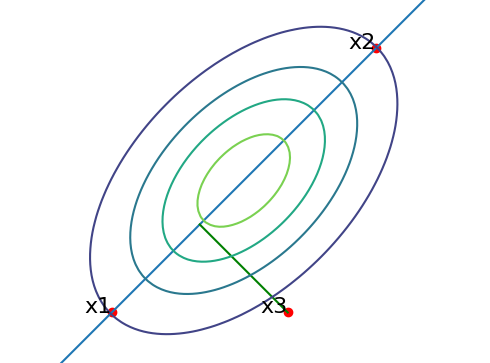
\includegraphics[scale=0.7]{./imgs/UNDX.png}
		\caption[UNDX による個体生成分布図]{ UNDX による個体生成分布図\label{fig:UNDX}}
	\end{center}
\end{figure}


\newpage


次に,4つ以上のより高次元での補間操作ではない理由を説明する.4つ以上の補間操作のほうが,高次元の空間を探索できるというメリットがある一方で,操作難度が高くなるというデメリットがある.平面UIにおける3つの個体の補間操作について,(\ref{eq:rex1})式で与える.
\begin{equation}\label{eq:rex1}
    \bm{x}^c = a*(\bm{x}_\mathrm{top} - \bm{x}_\mathrm{left\ bottom}) + b*(\bm{x}_\mathrm{right\ bottom} - \bm{x}_\mathrm{left\ bottom})
\end{equation}


ここで,$\mathbf{x}^c$は補間個体,$\mathbf{x}_\mathrm{top},\mathbf{x}_\mathrm{left\ bottom},\mathbf{x}_\mathrm{right\ bottom}$は補間操作UIにおける選択されたモデルであり,図\ref{fig:systemAno}においてUIの三角形の頂点と曲線で結ばれたモデルとが対応している.このとき重み変数$a,b$は(\ref{eq:weight})式が成り立つものとする.
\begin{equation}\label{eq:weight}
    \bm{p}_\mathrm{cursor} - \bm{p}_\mathrm{left\ bottom}  = a*(\bm{p}_\mathrm{top} - \bm{p}_\mathrm{left\ bottom}) + b*(\bm{p}_\mathrm{right\ bottom} - \bm{p}_\mathrm{left\ bottom})
\end{equation}
ここで, $\bm{p}_\mathrm{cursor}, \bm{p}_\mathrm{left\ bottom}, \bm{p}_\mathrm{top}, \bm{p}_\mathrm{right\ bottom}$はそれぞれ画面座標の原点から操作ポインタ,三角形UIの左下頂点,上頂点,右下頂点へのベクトルである.すなわち,左下頂点からポインタへのベクトルを上頂点,右下頂点方向の二つのベクトルで表すときの重みが$a,b$である.このようにすることで,$a,b$は行列計算で簡単に解く事が出来る.このように表すことで,操作ポインタと各頂点との距離が、補間対象の各モデルとの距離に対応するため,直感的な補間操作を行う事が出来る.しかし,これが4個以上での補間を二次元である平面 UI 上で実装しようとすると不都合が生じる.異なる四点を結ぶ三角錐状の三次元空間を二次元空間に射影しようとすると次元削減分の情報の損失が起こるため歪みが生じる.それを歪みなくかつドラッグで補間を表現するには,三角錐の断面を並行投影すればいいが,内部を全て探索できるようにするためには断面方向を回転させるといった別の操作が必要になり,操作難度が高くなる.


%\newpage

ここで,図\ref{fig:metahuman_cc2}に MetaHuman のブレンド操作について示す.図\ref{fig:metahuman_cc2}では現在作成しているキャラに加えて,4つのモデルをブレンド対象に使用している.しかし,計5つのモデルに対して補間操作を行っているわけではなく,実際には中心のモデルと,左の円環状に配置された4つのモデルのうち隣り合う二つの計3つのモデルの補間である.現在の対象は図左側のキャラのうち水色でハイライトした3人である.
このブレンド操作では,白のカーソルに近い位置3つのキャラのブレンドが行われる.
そのためカーソルが黄色の円内のどこに位置するかによって補間対象となるモデルが変わってしまう.現在セットされているのは4つのモデルのため,赤の線で4等分した領域ごとに補間対象のモデルが変わる.
現在カーソルが黄色の円内左下にいることから,ブレンド対象のキャラも中心のキャラから見て,左と下のキャラが対象になる.
このように既存のドラッグ操作による補間システムでも3種類が限界であるという事例から分かる通り,
平面のUIで4つ以上の直感的な補間操作を実現することは難しいため,今回は3つの補間操作を採用する.

\begin{figure}[h]
	\begin{center}
		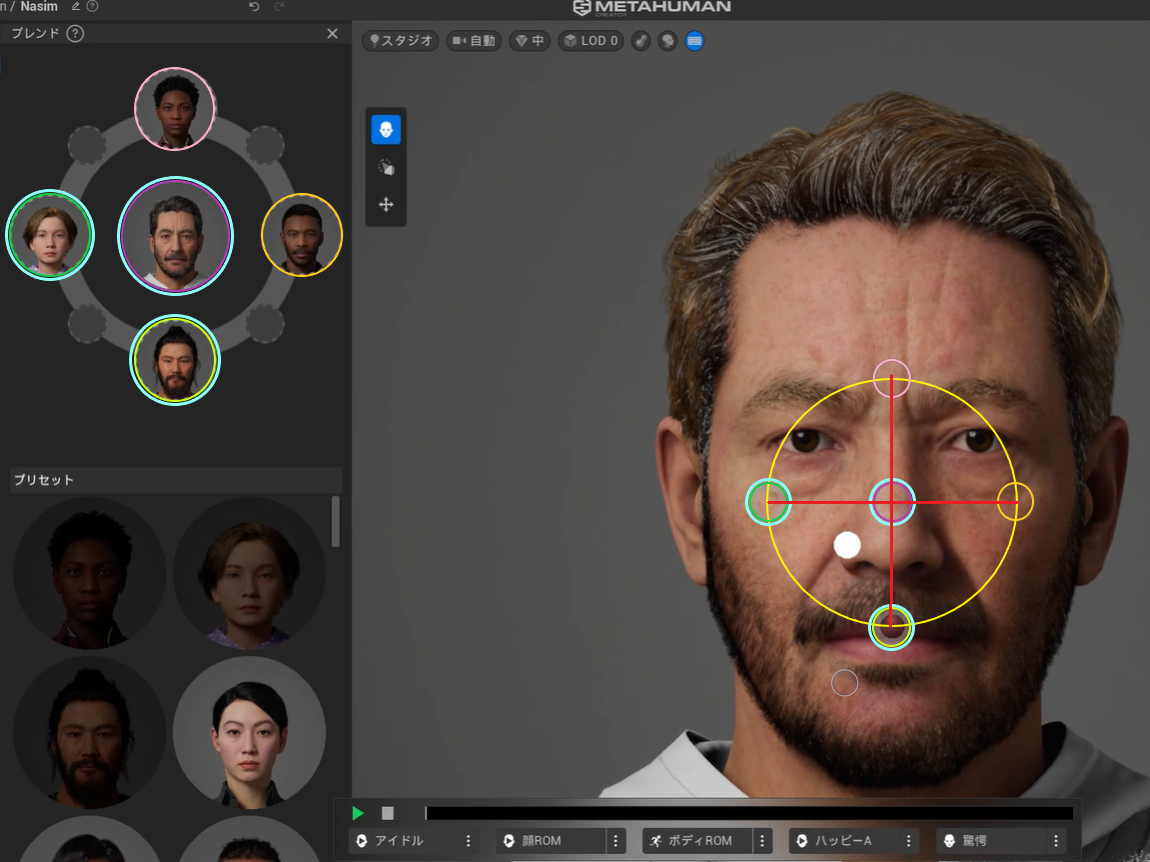
\includegraphics[scale=0.4]{./imgs/metahuman2.PNG}
		\caption{MetaHuman のブレンド操作\label{fig:metahuman_cc2}}
	\end{center}
\end{figure}

\clearpage
\section{IGA による次世代生成}

\subsection{選択}
選択操作は,エリート選択,トーナメント選択の両方によって行う.
エリート選択は補間によって決定されたモデルに対して,次の世代に何も変更を加えずに追加する.
トーナメント選択は選択された個体を親個体として,次の手順である交叉に全て使う.

\subsection{交叉}
交叉については多親交叉 REX を用いる.遺伝子数$n$に任意定数$k$を加えた$n+k$個の親を用いた交叉方法で,親個体群$\bm{x}^1,\bm{x}^2,...,\bm{x}^n+k$の重心を$\bm{x}^\mathrm{g}$としたとき,子個体$\bm{x}^c$は次の式で与えられる.
\begin{equation}\label{eq:rex1}
    \bm{x}^c = \bm{x}^\mathrm{g} + \sum_{i=1}^{n+k} \xi^i (\bm{x}^i - \bm{x}^\mathrm{g}) ,  \xi^i\sim\phi(0,\sigma^2_\xi)
\end{equation}
\begin{equation}\label{eq:rex2}
    \sigma^2_\xi = \frac{1}{n + k}
\end{equation}

この時,$\phi(0,\sigma^2_\xi)$は平均0,分散$\sigma^2_\xi$の確率分布であり,制限として(\ref{eq:rex2})式を満たすことが実数値 GA における設計指針において良い\cite{小林重信2009実数値}とされている.本提案では従来の手法に倣い,確率分布として一様分布を用いる.

\subsection{突然変異}
突然変異率1\%で遺伝子の値が別の値に置き換わるようにする.この値は通常の遺伝的アルゴリズムよりも大きく設定してある.理由として,多親交叉 REX\cite{小林重信2009実数値}での想定として,親個体数が遺伝子長よりも大きくするべきであると記述がある.しかし,本提案手法では親個体数が少ないために収束率が高くなってしまう.そこで突然変異率を上げることで多様性の維持をしつつも,収束は行えるような値に設定した.また,突然変異率が2\%を超えると個体群の分散が1世代で0.9倍程度しか収束しないことを事前に検証しており,世代数が増えてしまうのを防ぐために1\%とした.


また突然変異が起こった際に,変化する値については以下の$(\kappa,\mu)=(0.5,0)$のフォンミーゼス分布\cite{vonMisesDist}を正規化したものに従うものとする.(\ref{eq:von1}),(\ref{eq:von2}),(\ref{eq:von3})式に累積分布関数,確率密度関数,j次の第一種変形ベッセル関数について示す.$\mu$は角度方向のパラメータであり, $[0\mathrm{rad},2\pi \mathrm{rad}]$の間で確率密度における
ピークの方向を示す. $\kappa$は濃度パラメータで,大きいほどピークが高くなる.この時に方向を示す実数値$\theta$がとる確率は$F(\theta)$で表される.図\ref{fig:vonMises50000}に50000サンプルの度数分布表を示す.図\ref{fig:vonMises50000}から見て分かる通り,V字型の確率分布になっている.この確率分布を利用する.提案手法では補間を行う関係上,補間幅が広い方が多くの領域を探索出来ることになるため,補間幅が広くなるような値である定義域の端に近い値に変異してほしいと考えた.従って,一様分布ではなくV字型の分布を持つものを採用する.V字型の分布の中でフォンミーゼス分布を利用する理由として,本システムの実装に用いた Python で容易に実装出来るからである.

\begin{equation}\label{eq:von1}
F(\theta) = \frac{1}{2\pi I_{0}(\kappa)} \left[\theta I_{0}(\kappa) + 2 \sum_{j=0}^{\infty} \frac{I_{j}(\kappa) \sin(j(\theta - \mu))}{j}\right]
\end{equation}
\begin{equation}\label{eq:von2}
f(\theta) = \frac{\exp\{\kappa \cos(\theta - \mu)\}}{2\pi I_{0}(\kappa)}
\end{equation}
\begin{equation}\label{eq:von3}
I_{j}(\kappa) = \left(\frac{\kappa}{2}\right)^{j} \sum_{i=0}^{\infty} \frac{\left(\frac{\kappa^{2}}{4}\right)^{i}}{i!\Gamma(j+i+1)}
\end{equation}

\begin{figure}[h]
	\begin{center}
		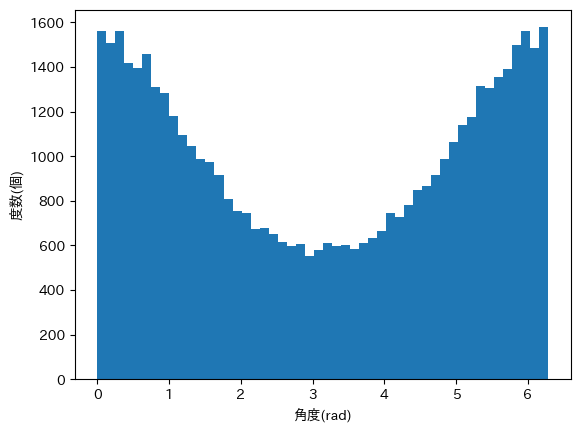
\includegraphics[scale=0.55]{./imgs/vonMisesDis50000.png}
		\caption{フォンミーゼス分布のヒストグラム(sample size = 50000)\label{fig:vonMises50000})}
	\end{center}
\end{figure}
\newpage

\subsection{サブ集団}
IGA における一世代における個体数は24個体に設定し,サブ集団は6個体ずつに4つのサブ集団に分ける.この個体数に関しては,単純なGAであれば20から40個体で十分であるという研究報告\cite{grefenstette1986optimization}があり, IGA の時間的制約のためなるべく小さくしたいという理由からである.またサブ集団の個数設定について,補間を行う個体が3つであるのでその倍数にしたかったという点と,モデリングの際に対象となるモデル以外をあまり多く配置してしまうと,画面を圧迫するために少なくしたかったという点からである.
このようにサブ集団に分けて並列的に行われる手法を島モデル型分散遺伝的アルゴリズム\cite{tanese1989distributed}という.
ただし,本研究では, IGA における一度に提示する提案モデル数の削減が主目的である.
島モデル型では,選択や交叉など各サブ集団ごとに行われるが,
本システムに用いる交叉手法である多親交叉REXは親の数が多く求められるので親個体を分けて交叉はしない.


ここで$k$世代目の$m$番目のサブ集団における補間個体を${\bm{x}^k_m}_\mathrm{elite}$とするとき,表\ref{tb:nextSub}のように$k+1$世代生成を行う.また,図\ref{fig:subFlow}にネットワーク図を示す.

\begin{table}[h]
	\centering
	\caption{$k+1$世代目の個体群\label{tb:nextSub}}
	\scalebox{1.0}{
		\begin{tabular}{|c|c|c|} \hline
                サブ集団番号&エリート個体&交叉生成される個体数\\ \hline\hline
                1&${\bm{x}^k_1}_\mathrm{elite}$&5\\ \hline
                2&${\bm{x}^k_2}_\mathrm{elite}$&5\\ \hline
                3&${\bm{x}^k_3}_\mathrm{elite}$&5\\ \hline
                4&${\bm{x}^k_1}_\mathrm{elite}, {\bm{x}^k_2}_\mathrm{elite}, {\bm{x}^k_3}_\mathrm{elite}, {\bm{x}^k_4}_\mathrm{elite}$&2\\ \hline
		\end{tabular}
	}
\end{table}

\begin{figure}[h]
	\begin{center}
		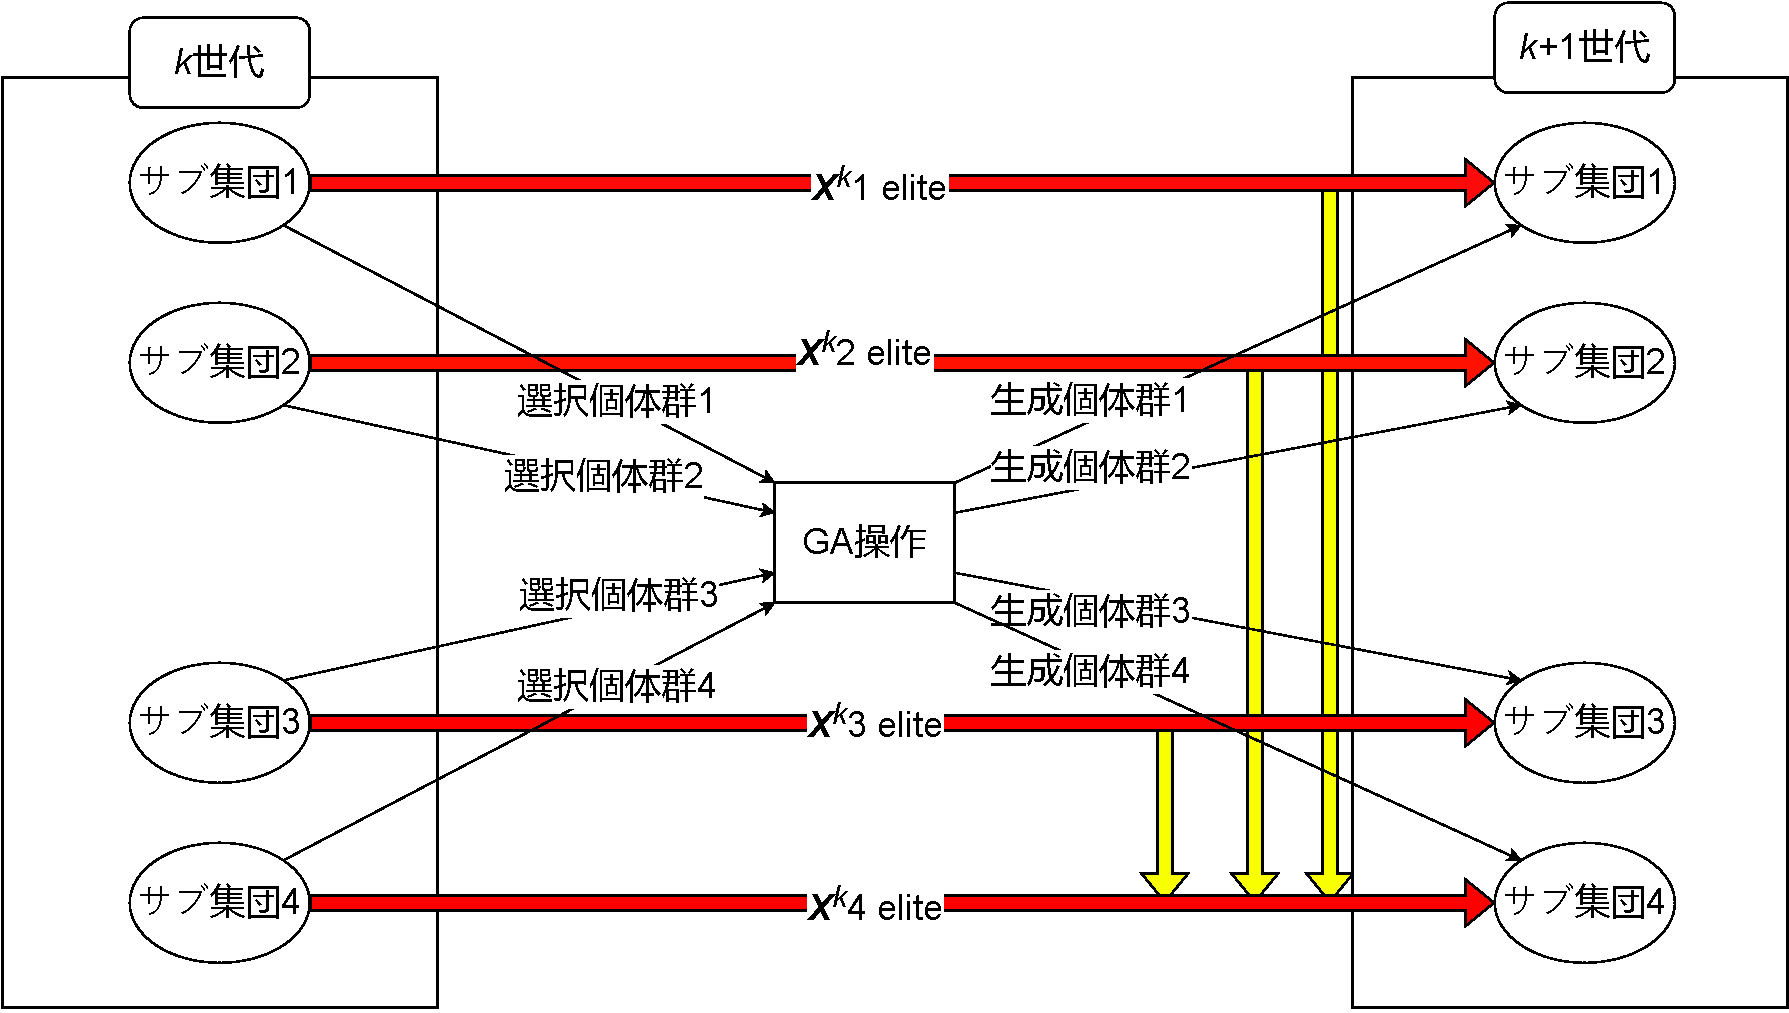
\includegraphics[scale=0.4]{./imgs/subFlow.pdf}
		\caption{次世代生成のネットワーク図\label{fig:subFlow}}
	\end{center}
\end{figure}
つまり,サブ集団1,2,3については1世代前の同サブ集団からエリート個体を引き継ぎ,サブ集団4については1世代前のエリート個体すべてを引き継ぎ,各サブ集団の個体数が6個体になるように個体生成された子個体で埋めた.

このとき24個体中,交叉生成をした子個体は17個体であり,交叉率は71\%である.
1ステップ前に制作したモデルを一新し,前世代のエリート個体を再び提案モデルとして登場させることで,過去の考えを組みつつも新しい発想が生み出されていくことを期待する.加えて,エリート個体をすべて引き継ぐサブ集団4を用意することでより洗練されたモデルが生み出されることを望む.

\newpage

\section{微調整操作}
この操作はプロシージャルモデリングのパラメータを直接操作するという,従来の方法であり,操作パラメータ数の削減という本研究の目的を逸脱している.しかし,提案モデルにユーザが欲しいと思う特徴がない時や,あと少し手を加えたいといったことについて,本システムは補間操作およびIGAによるモデル提案という性質上,そのような細かいモデリングを行うことは難しい.そのため基本操作上ではパラメータ操作のUIは隠しつつも,必要であれば表示して操作が出来るようにすることで,大まかな補間操作に加えて細かいパラメータ調整を適宜行えるようにした.


ただし,この操作は補間モデルだけでなく,選択モデルに対しても行う.なぜなら,補間モデルに対してパラメータ操作した差分を選択モデルに対しても操作をすることで,補間としての体裁を保つことが出来る.また,個別で調整するということはそのパラメータがユーザにとって重要度が高いと言える.そのため,親個体にその要素を引き継ぐ必要がある.以上の2点からパラメータ調整した差分は選択モデルに対しても適用する.

\section{システムインターフェース}
本節ではシステムインターフェースについて,各操作を3段階ずつ示すことで,操作に対する動作を説明する.
図\ref{fig:systemOverViewInit}はシステムの初期状態である.左下に UI ,
中心のモデルが操作されるモデル,右6つのモデルが提案されるモデル,左3つは補間対象であるモデルが表示される.


まず図\ref{fig:systemOverViewSelect}に選択操作を示す.選択は左下,上,右下の順に行われ各補間モデルにセットされる.次に図\ref{fig:systemOverViewInter}に補間操作を示しており,今回は左下頂点から上頂点と右下頂点の中間に向かうような操作をしている.$a,b$は3.1.3.2の補間操作に示した重み係数である.また,直前の画面である図\ref{fig:sOV_select3}では$a=0.00,b=0.00$であり,これは赤色のポインタは左下頂点に位置することを示しており,新たにモデルが提案される度にその位置にリセットされる.
最後に図\ref{fig:systemOverViewAdj}にケーキの切り取る角度を表すパラメータ( Cake cut )を0.8から0.4に減らす調節操作を示す.この時,左側の補間対象のモデルもその差分だけケーキの大きさが小さくなっていく様子が確認できる.

\begin{figure}[h]
	\begin{center}
		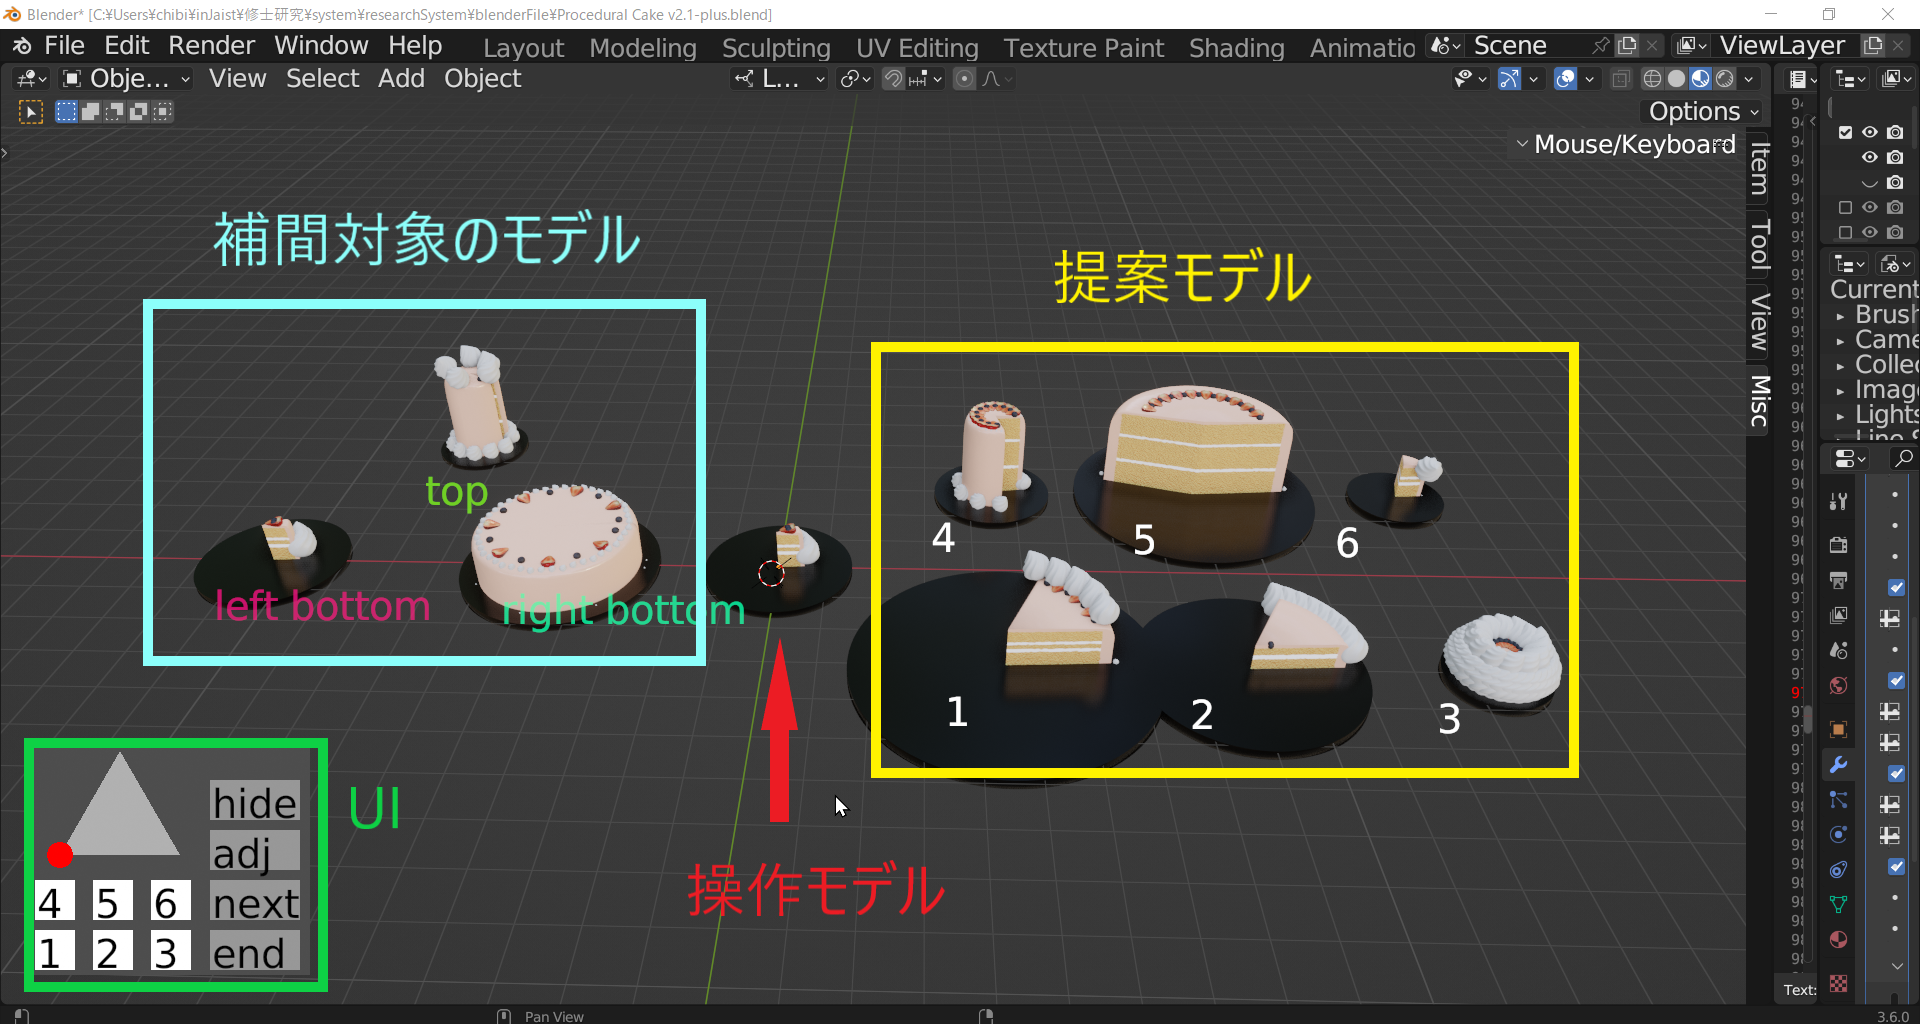
\includegraphics[scale=0.25]{./imgs/systemUse/init.png}
            \caption{システムの初期状態}\label{fig:systemOverViewInit}
	\end{center}
\end{figure}



\begin{figure}
  %\ContinuedFloat % 前の figure を継続
  \centering
  \begin{subfigure}{1\linewidth}
    \centering
    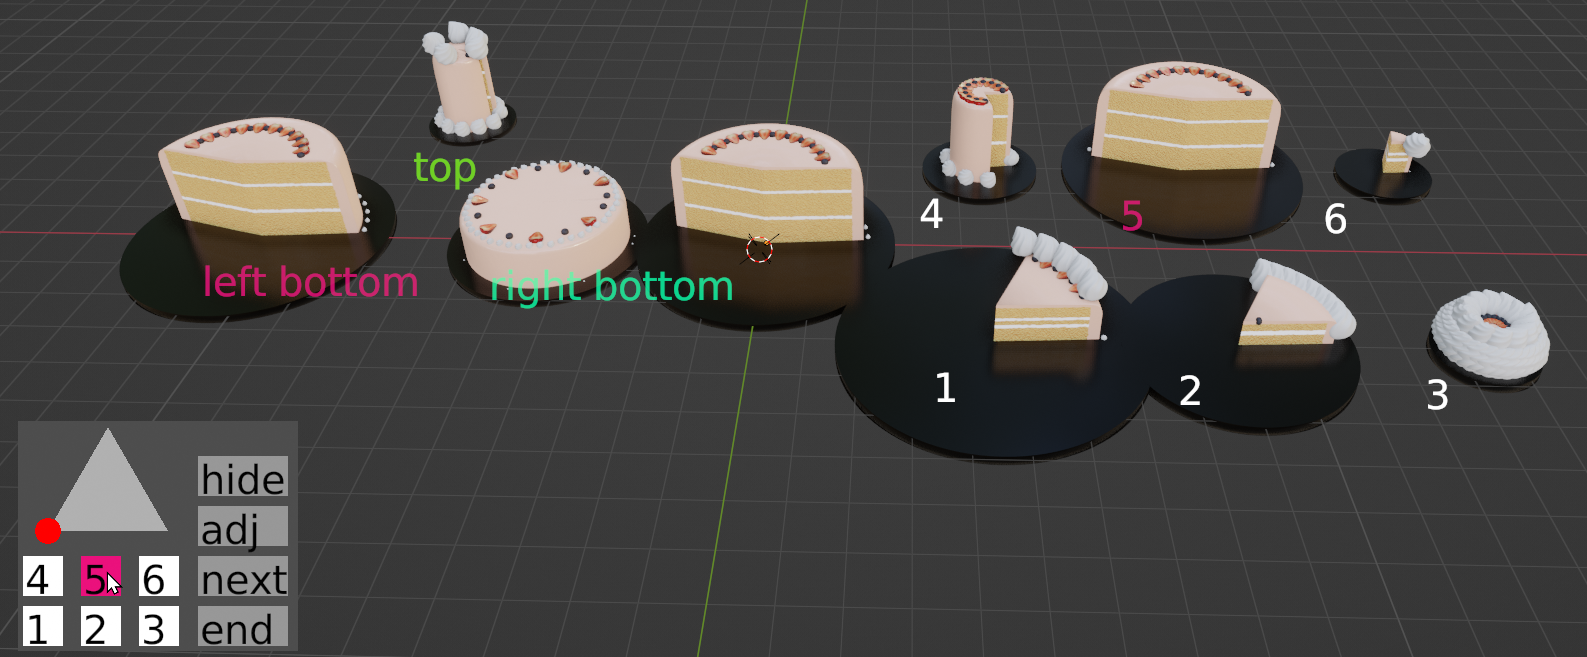
\includegraphics[scale=0.33]{./imgs/systemUse/select1.png}
    \caption{左下頂点に提案モデル5を選択}\label{fig:sOV_select1}
  \end{subfigure}\\
  \begin{subfigure}{1\linewidth}
    \centering
    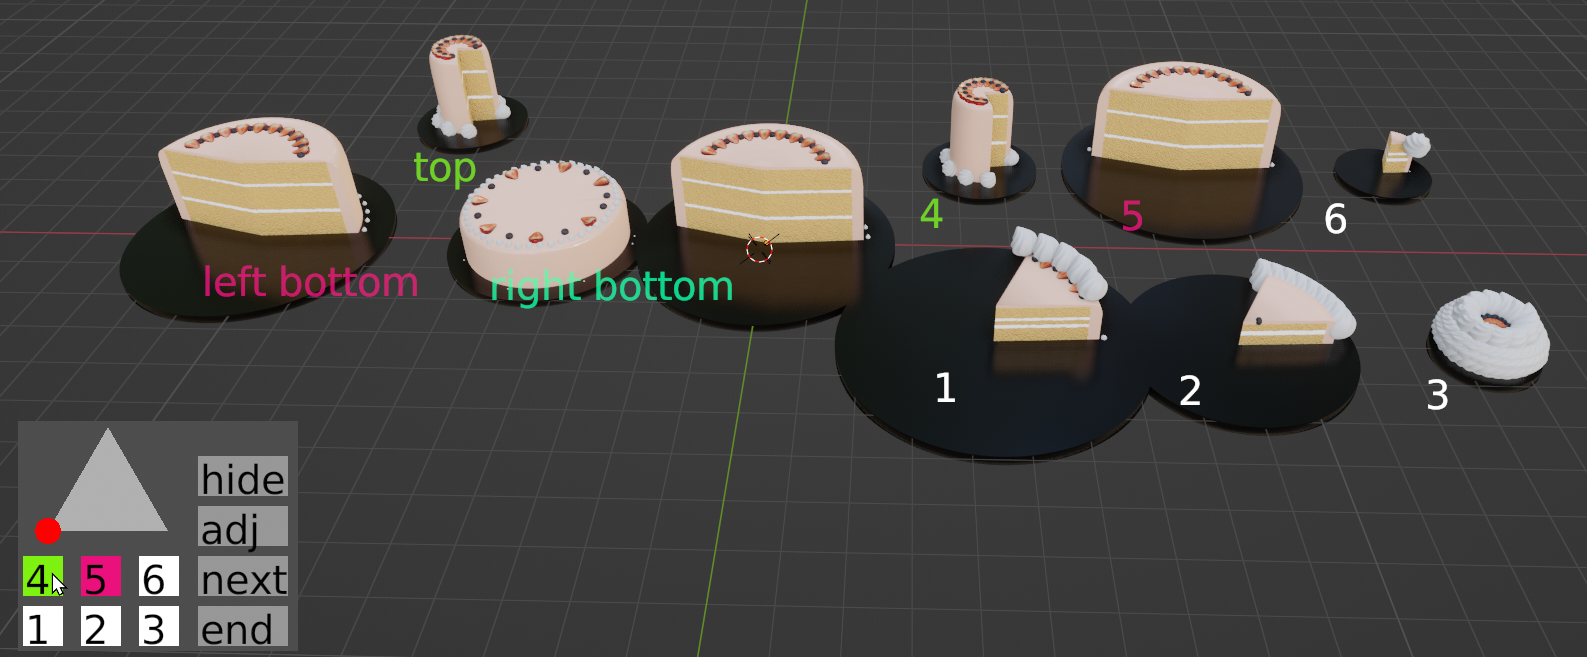
\includegraphics[scale=0.33]{./imgs/systemUse/select2.png}
    \caption{上頂点に提案モデル4を選択}\label{fig:sOV_select2}
  \end{subfigure}\\
  \begin{subfigure}{1\linewidth}
    \centering
    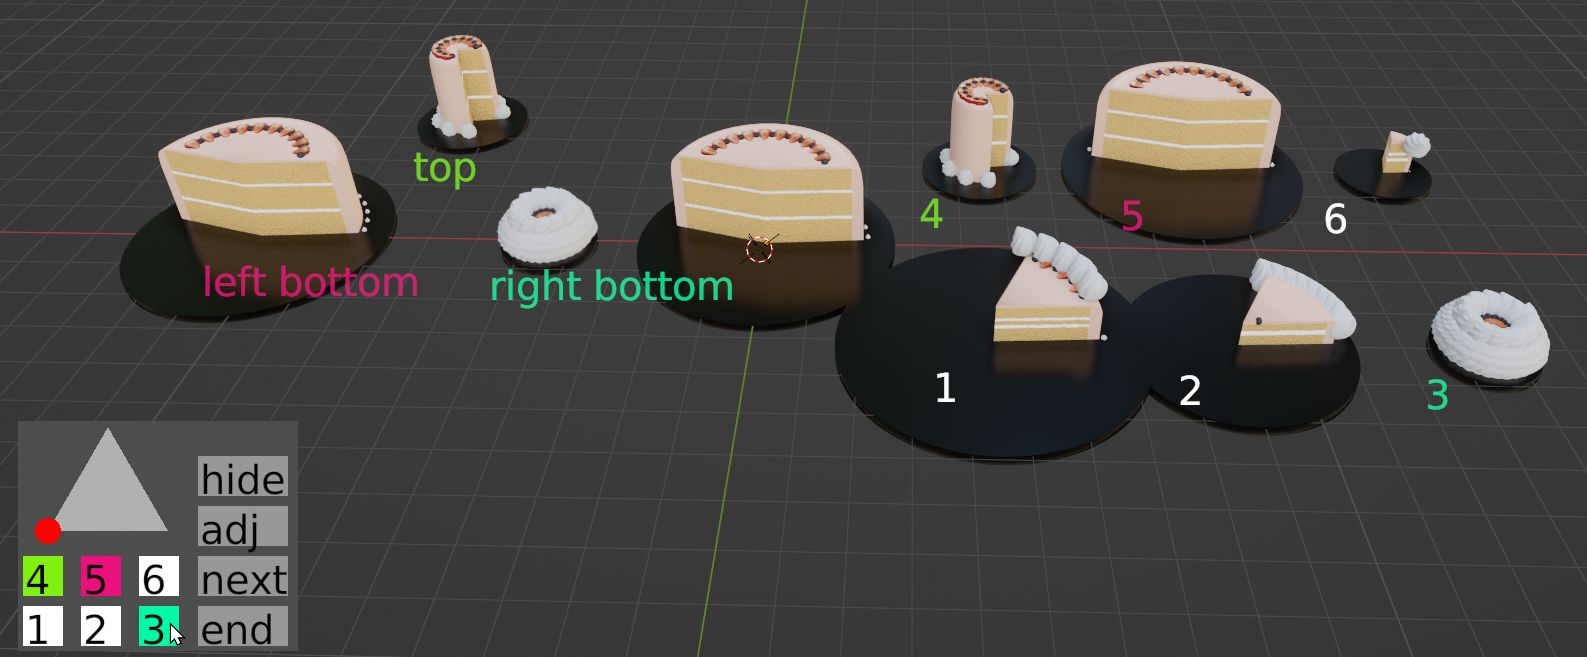
\includegraphics[scale=0.33]{./imgs/systemUse/select3.png}
    \caption{右下頂点に提案モデル3を選択}\label{fig:sOV_select3}
  \end{subfigure}\\
  \caption{実装システムの選択操作}\label{fig:systemOverViewSelect}
\end{figure}

\begin{figure}
  %\ContinuedFloat % 前の figure を継続
  \centering
  \begin{subfigure}{1\linewidth}
    \centering
    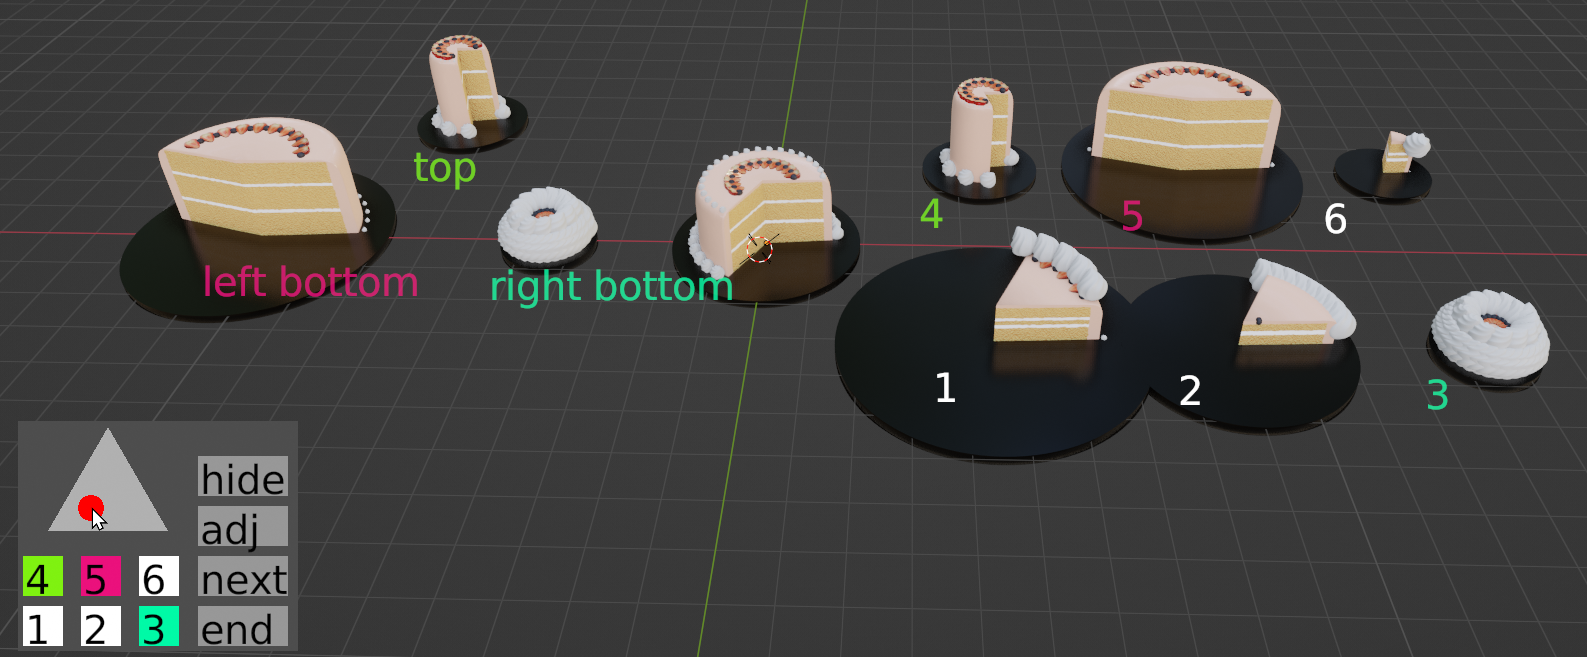
\includegraphics[scale=0.33]{./imgs/systemUse/inter1.png}
    \caption{補間操作($a=0.22,b=0.24$)}\label{fig:sOV_inter1}
  \end{subfigure}\\
  \begin{subfigure}{1\linewidth}
    \centering
    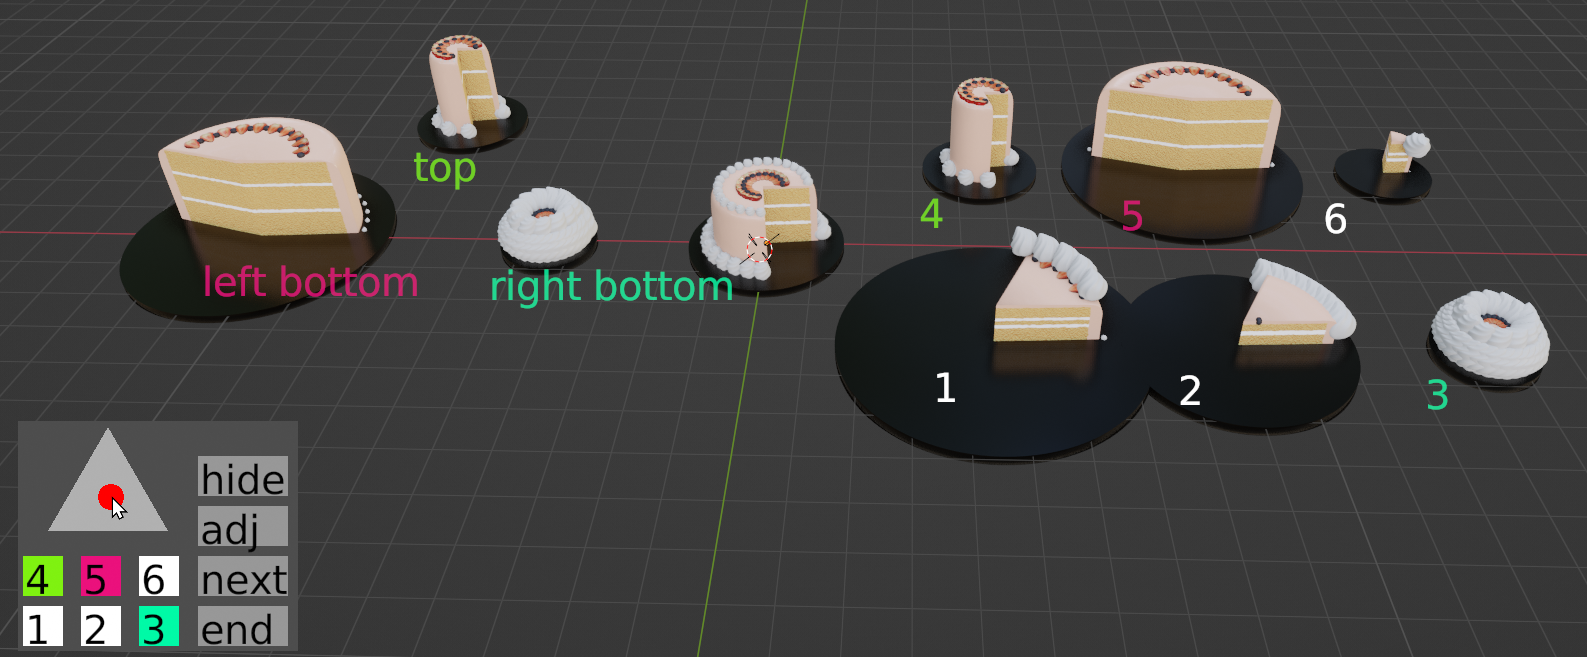
\includegraphics[scale=0.33]{./imgs/systemUse/inter2.png}
    \caption{補間操作($a=0.32,b=0.36$)}\label{fig:sOV_inter2}
  \end{subfigure}\\
  \begin{subfigure}{1\linewidth}
    \centering
    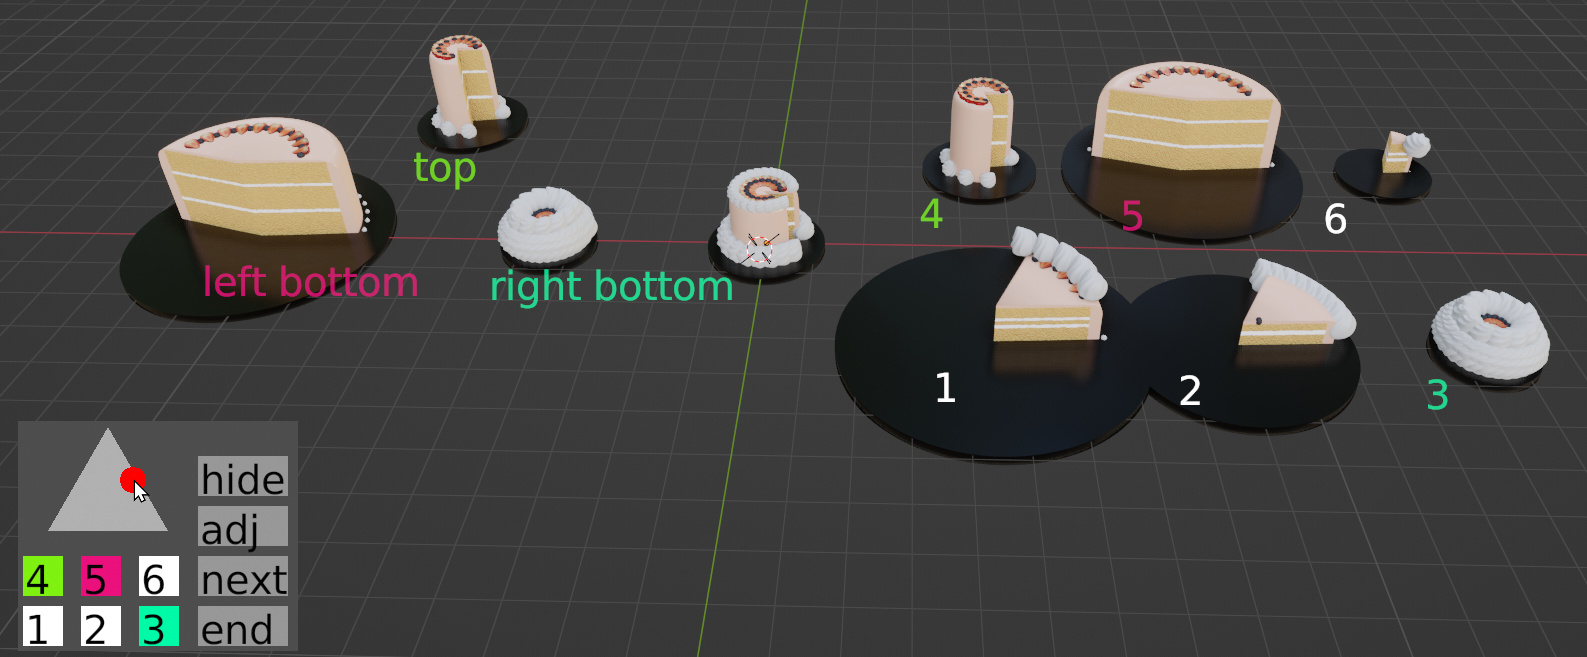
\includegraphics[scale=0.33]{./imgs/systemUse/inter3.png}
    \caption{補間操作終了($a=0.49,b=0.46$)}\label{fig:sOV_inter3}
  \end{subfigure}\\
  \caption{実装システムの補間操作}\label{fig:systemOverViewInter}
\end{figure}

\begin{figure}
  %\ContinuedFloat % 前の figure を継続
  \centering
  \begin{subfigure}{1\linewidth}
    \centering
    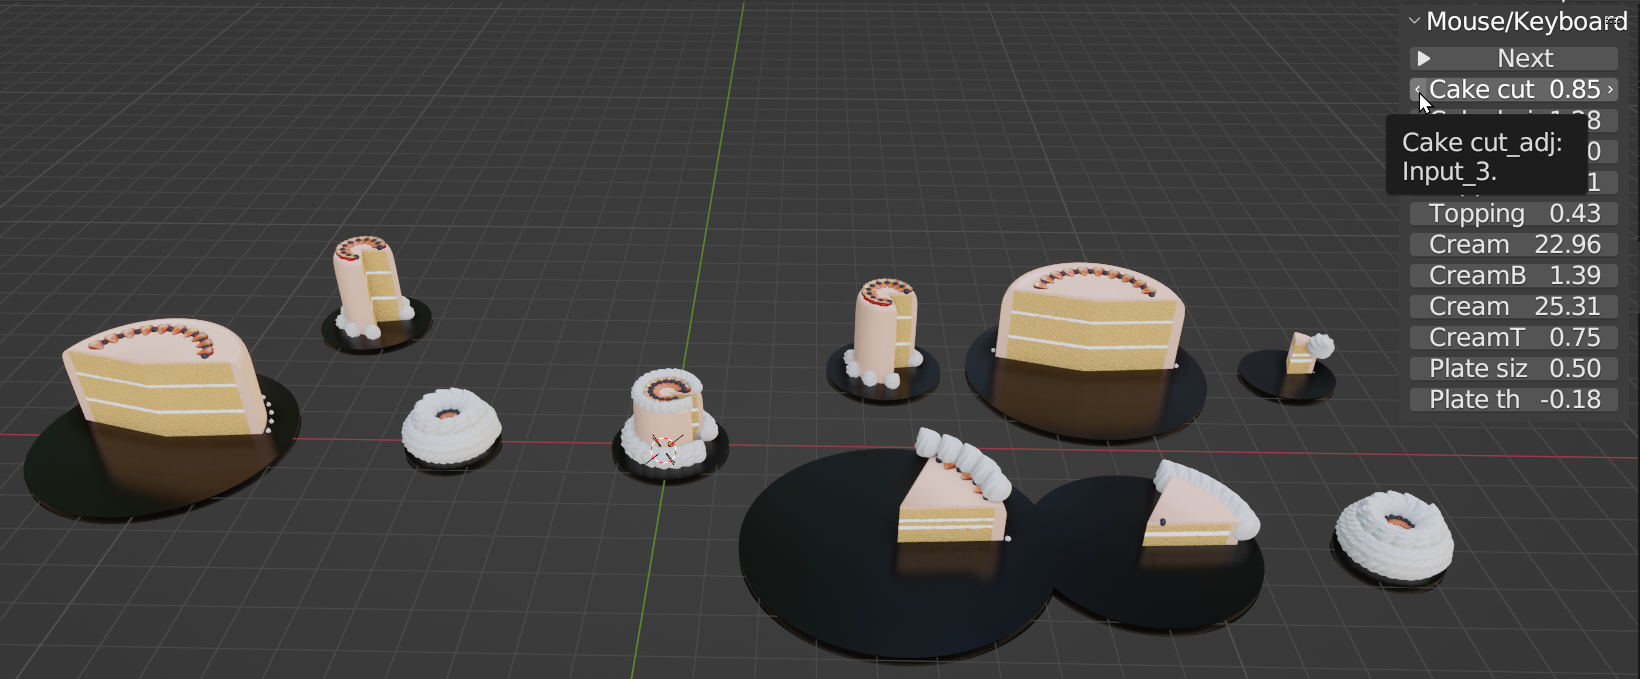
\includegraphics[scale=0.33]{./imgs/systemUse/adj0.png}
    \caption{微調整前(Cake cut = 0.85)}\label{fig:sOV_adj0}
  \end{subfigure}\\
  \begin{subfigure}{1\linewidth}
    \centering
    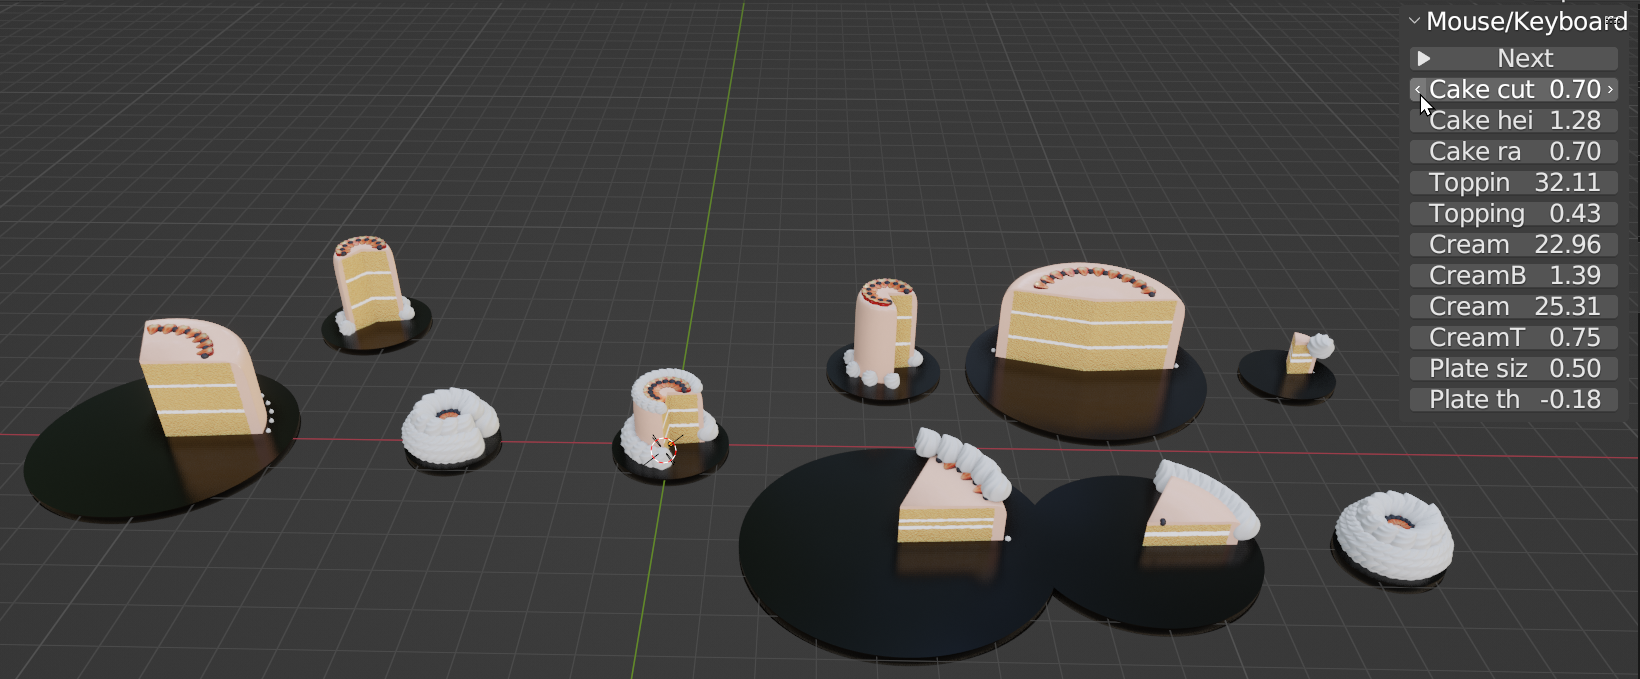
\includegraphics[scale=0.33]{./imgs/systemUse/adj1.png}
    \caption{微調整操作(Cake cut = 0.70)}\label{fig:sOV_adj1}
  \end{subfigure}\\
  \begin{subfigure}{1\linewidth}
    \centering
    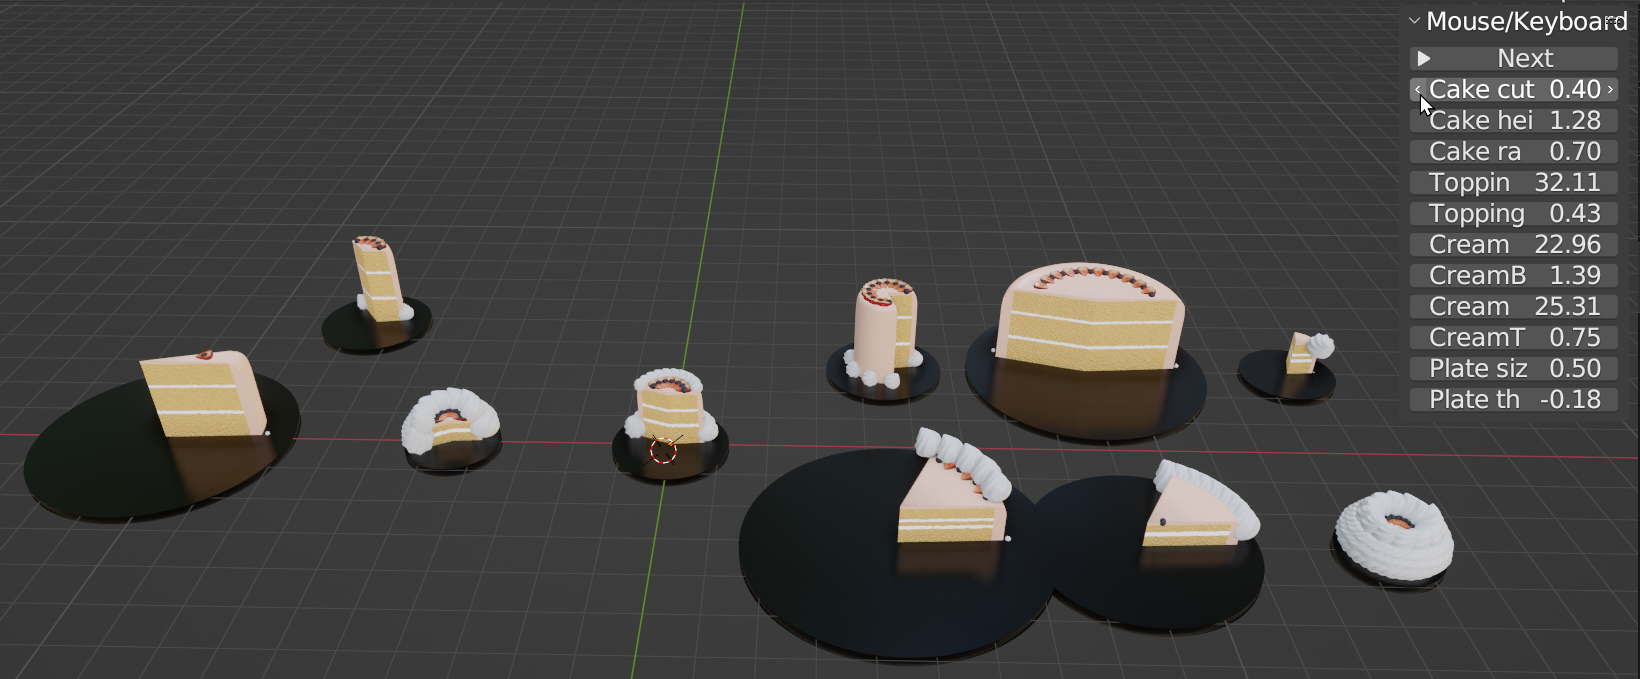
\includegraphics[scale=0.33]{./imgs/systemUse/adj3.png}
    \caption{微調整操作終了(Cake cut = 0.40)}\label{fig:sOV_adj2}
  \end{subfigure}\\
  \caption{実装システムの微調整操作}\label{fig:systemOverViewAdj}
\end{figure}

\clearpage

\newpage

\chapter{実験}

本章では,3章において提案されたシステムの評価実験について述べる.まず,実験に関する具体的な設定と定性評価のためのアンケート項目を示す.その後,実験結果について定性,定量の順で考察を交えつつ述べ,最後に提案システムの評価を総括する.

\section{実験方法}
提案システムを評価するために,20代から30代の男女計11人(男9人,女2人)にユーザ実験の協力をしていただいた.また,被験者の中で Blender などの DCC ツールの経験があるのは6人であった.提案システムと対照実験用のシステムに対して,二つのモデリングタスクを行った後,使用感に関するアンケートに答えてもらった.

二つのモデリングタスクは予め用意した画像に近づけるようにモデリングしてもらうタスクと,ユーザが満足するまで完全に自由にモデリングをしてもらうタスクである.それぞれの意図として,コンテンツ制作には多人数で行う場合と個人で行う場合とがあり,多人数で行うときには予め完成イメージを共有したうえで行うのに対して,個人での場合は制約なく行うからであり,二つのタスクはこの2パターンの簡易的な再現を行っている.

本実験における評価について,システム操作時間とプロシージャルモデリングのパラメータ変化による定量評価および,アンケートによる定性評価から提案システムの有意性について議論を行う.

\subsection{実験環境}
本提案手法では,3DCGのモデリングを実験するにあたり,複数のオブジェクトを同時に見ることや,変形における動作ラグが予測される.まず,表\ref{tb:pcEnv}システム使用時のPC環境を以下に示す.
\begin{table}[h]
	\centering
	\caption{PC 環境\label{tb:pcEnv}}
	\scalebox{1.0}{
		\begin{tabular}{|c||c|} \hline
                OS&Windows 11 Home\\ \hline
			CPU&12th Gen intel(R) Core(TM) i7-12700\\ \hline
                RAM&32GB\\ \hline
			GPU&NVIDIA GeForce RTX 3080\\ \hline\
			画面サイズ&27inch\\ \hline
                解像度&2560$\times$1440\\ \hline\hline
			ソフト&Blender 3.6.7\\ \hline
		\end{tabular}
	}
\end{table}
\subsection{実験設定}
実験設定について,二種類のモデリングタスクおよび,対照実験について説明する.

\subsubsection{実験1}
実験1では,あらかじめ制作された目標モデルの画像を見て,それに近いモデルを作ってもらうタスクを設定した.対象とするモデルは HuyKhoi2407 によって作成された Procedural Cake \footnote[4]{\url{https://blendermarket.com/products/procedural-cake--blender-geometry-nodes} } で,パラメータ数は11である.以降 Cake モデルと呼ぶ.表\ref{tb:cakeParam}にパラメータの名前,data type,範囲 および制作してもらう目標モデルのパラメータを示す.また,図\ref{fig:cake1}に実際に被験者に参考にしてもらった画像について示す.パラメータの名前からも分かる通り,ケーキについてカットする角度や,ホール,クリームなどの大きさ,トッピングの数や皿の状態を指定する事が出来る.本モデルを選んだ理由として,パラメータを動かしたときにモデルの外観との対応が非常に分かりやすく,パラメータ数が11と比較的少ないことが挙げられる.また,実際にパラメータが最大最小を取るときの外観について\hyperref[paramMean]{付録A}に掲載する.

\begin{table}[h]
	\centering
	\caption{Cake モデルのパラメータ\label{tb:cakeParam}}
	\scalebox{1.0}{
		\begin{tabular}{|c|c|c|c||c|} \hline
                name&data type&min&max&目標モデル\\ \hline\hline
			Cake cut&Float&0.0&1.0&0.782\\ \hline
                Cake height&Float&0.5&2.0&1.03\\ \hline
                Cake radius&Float&0.5&2.0&1.00\\ \hline
                Topping quantity&Float&0.0&50.0&41.3\\ \hline
                Topping position&Float&0.0&1.0&0.314\\ \hline
                CreamBot quantity&Float&0.0&50.0&29.2\\ \hline
                CreamBot Size&Float&0.0&2.0&1.46\\ \hline
                CreamTop quantity&Float&0.0&50.0&15.9\\ \hline
                CreamTop Size&Float&0.0&2.0&0.900\\ \hline
                Plate size&Float&0.3&1.0&0.645\\ \hline
                Plate thickness&Float&-0.2&-0.1&-0.159\\ \hline
                
		\end{tabular}
	}
\end{table}


\begin{figure}
\vspace{-2cm}
\centering
\begin{tabular}{c}
  \begin{minipage}{.7\linewidth}
    \centering
    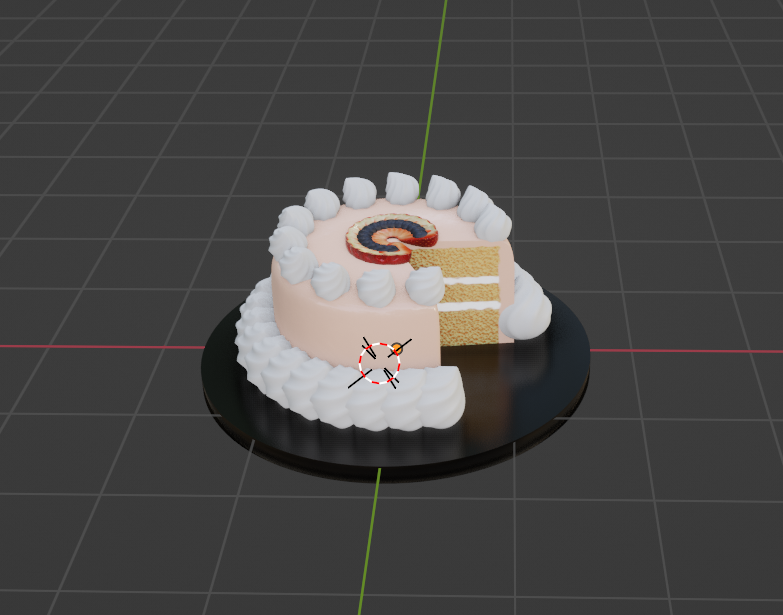
\includegraphics[scale=0.45]{./imgs/cakeSample/cake1.png}
    \subcaption{正面}
  \end{minipage}\\ 
  \begin{minipage}{.7\linewidth}
    \centering
    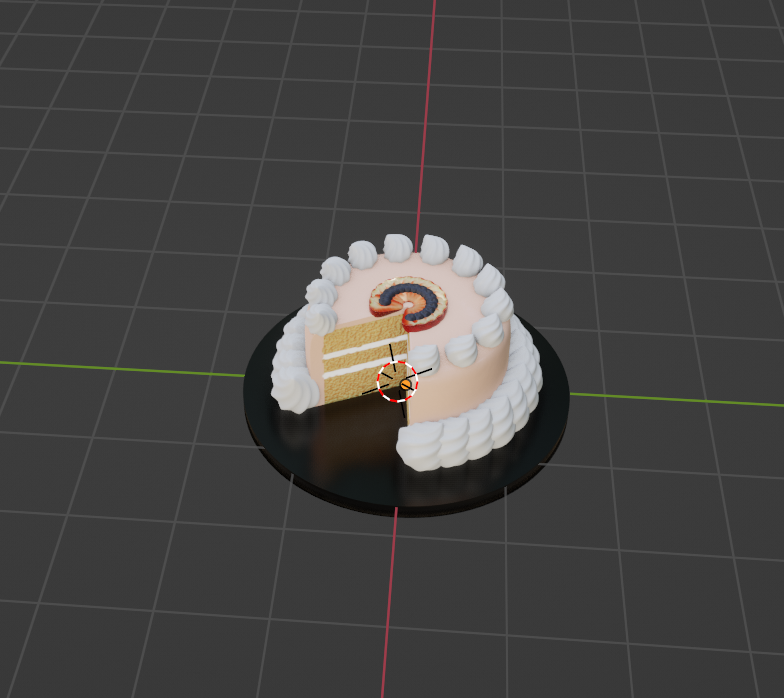
\includegraphics[scale=0.45]{./imgs/cakeSample/cake2.png}
    \subcaption{右}
  \end{minipage}\\ 
  \begin{minipage}{.7\linewidth}
    \centering
    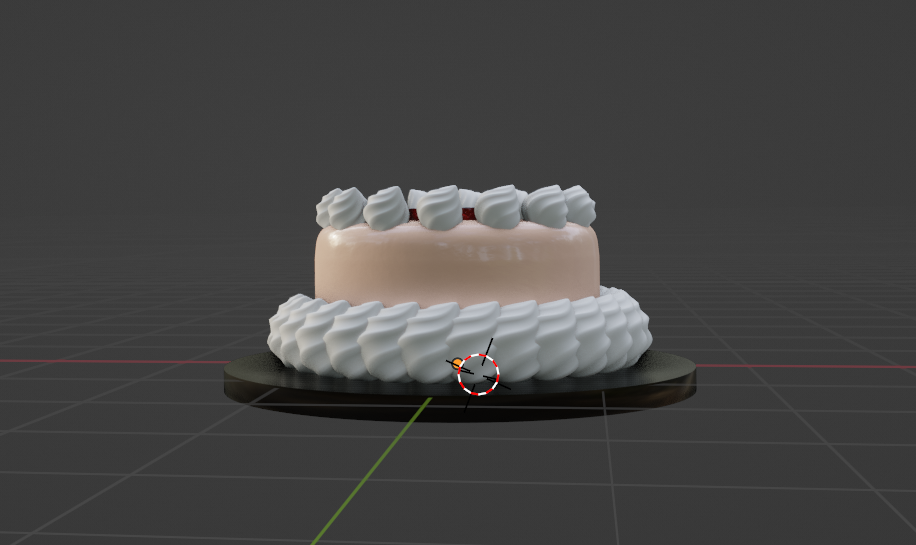
\includegraphics[scale=0.4]{./imgs/cakeSample/cake3.png}
    \subcaption{背面}
  \end{minipage}
\end{tabular}
\caption{目標の Cake モデルの外観}\label{fig:cake1}
\end{figure}

\clearpage
\newpage

\subsubsection{実験2}
実験2では,実験1のような明確な目的を用意せずに自由にモデリングを行ってもらうタスクを設定した.対象とするモデルは Blender Bash によって作成された Procedural Furniture Chair - Sofa - Table - Bed \footnote[5]{\url{https://blendermarket.com/products/procedural-furniture-chair---sofa---table---bed} }で,パラメータ数は25とある程度大きなモデルを利用する.以降 Sofa モデルと呼ぶ.表\ref{tb:sofaParam}にパラメータの名前, data type, 範囲を示す.図\ref{fig:sofa1}に Sofa モデルの一例について示す.また,実際にパラメータが最大最小値を取るときの外観について\hyperref[paramMean]{付録A}に掲載する.パラメータ名に
"NO / 1 / YES"とあるものは,本体のモデルの横に,壁あるいはクッションを付属するためのパラメータであり,パラメータが0(= NO)の時は何もなし,1はモデルの正面向かって左側のみに,2(= YES)の時は両側につけるものとなっている.

\begin{figure}[h]
\centering
\begin{tabular}{c}
  \begin{minipage}{.7\linewidth}
    \centering
    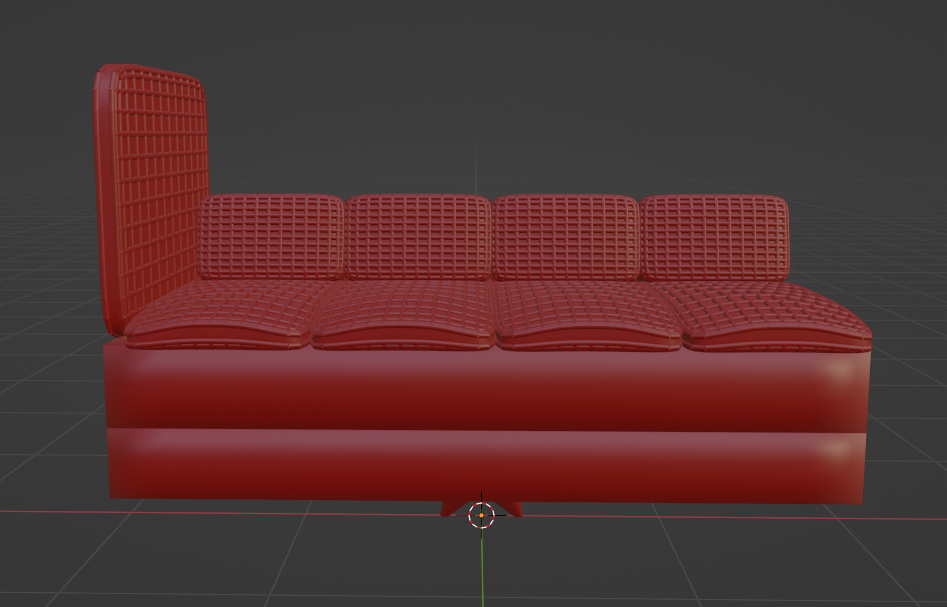
\includegraphics[scale=0.27]{./imgs/sofaSample/sofa1.png}
    \subcaption{正面}
  \end{minipage}\\ \\
  \begin{minipage}{.7\linewidth}
    \centering
    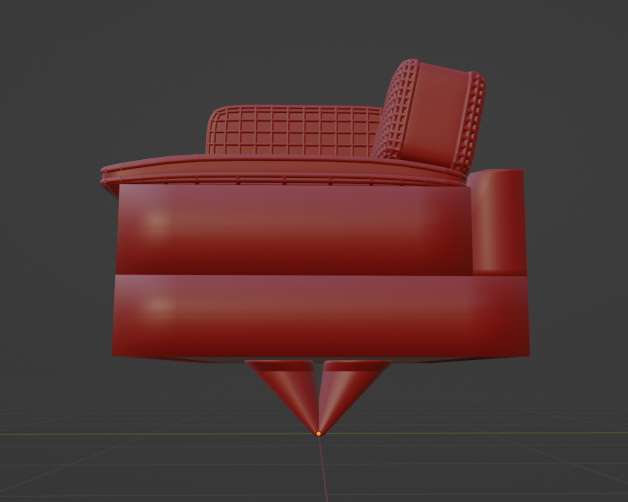
\includegraphics[scale=0.35]{./imgs/sofaSample/sofa2.png}
    \subcaption{右}
  \end{minipage}
\end{tabular}
\caption{sofa モデルの一例}\label{fig:sofa1}
\end{figure}

\begin{table}[h]
	\centering
	\caption{Sofa モデルのパラメータ\label{tb:sofaParam}}
	\scalebox{1.0}{
		\begin{tabular}{|c|c|c|c|} \hline
                name&data type&min&max\\ \hline\hline
			Depth&Float&0.2&4.0\\ \hline
                Width&Float&0.3&5.0\\ \hline\hline
                Legs height&Float&0.01&1.0\\ \hline
                Leg shape&Float&0.0&20.0\\ \hline
                Leg diameter&Float&0.01&0.04\\ \hline
                Leg angle&Float&0.0&1.0\\ \hline
                Leg position&Float&0.02&5.0\\ \hline\hline
                Base height&Float&0.01&0.5\\ \hline
                Base2 height&Float&0.01&0.5\\ \hline\hline
                Back thickness&Float&0.01&0.3\\ \hline
                Back/Side height&Float&0.01&1.5\\ \hline\hline
                Side NO / 1 / YES&Int&0&2\\ \hline
                Side thickness&Float&0.02&0.03\\ \hline\hline
                N. of Cushions&Int&0&5\\ \hline
                Cushion thickness&Float&0.05&0.5\\ \hline
                Cushion nosing&Float&0.0&0.3\\ \hline\hline
                Back Cushion height&Float&0.1&0.7\\ \hline
                Back Cush. Thickness / *Puffiness&Float&0.05&0.5\\ \hline\hline
                Side Cushions NO / 1 / YES&Int&0&2\\ \hline
                Side Cushion Height&Float&0.1&1.8\\ \hline
                Side Cushion Thickness&Float&0.05&0.5\\ \hline\hline
                Cushion Stitching&Float&0.0&0.05\\ \hline
                Cushion Crease&Float&0.0&0.3\\ \hline
                Bevel&Float&0.001&1.0\\ \hline
                Subd&Int&0&2\\ \hline
                
		\end{tabular}
	}
\end{table}


\clearpage
\newpage

\subsection{対照実験}
対照実験では,\hyperref[label:relatedResearch]{2.1.2の関連研究}でも紹介した,BO as Assistant \cite{koyama2022bo}という手法と比較する.システム設計として,基本のプロシージャルモデリングと同じ動作が出来る上に,補間操作という提案システムの要素も持ち合わせているこの手法が対照実験として適していると考えた.また,koyama らは図\ref{fig:boAssistant1}に示すように Mac OS 上でのシステム設計を公開している.それにならい,図\ref{fig:boAssistant2}に Windows OS 上で実装しなおしたものを示す.画像の奥のモデルについて左から順番に Suggestion1, Suggestion2, Suggestion3 とし,それについて,画像右側のパラメータを0から1に動かすことで,操作モデルとの補間を行う事が出来る.そして Next ボタンを押すことで次の提案モデルが生成される.また,先行研究で実装されていたシステムでは一度提案モデルの補間を行った直後に Next ボタンを押したときと同様に次の提案モデルへの変更が起こる仕様であったが,実装の都合上補間操作後, Next ボタンを押さない限り次の提案モデルに切り替わらないようになっている.
\begin{figure}[h]
	\begin{center}
		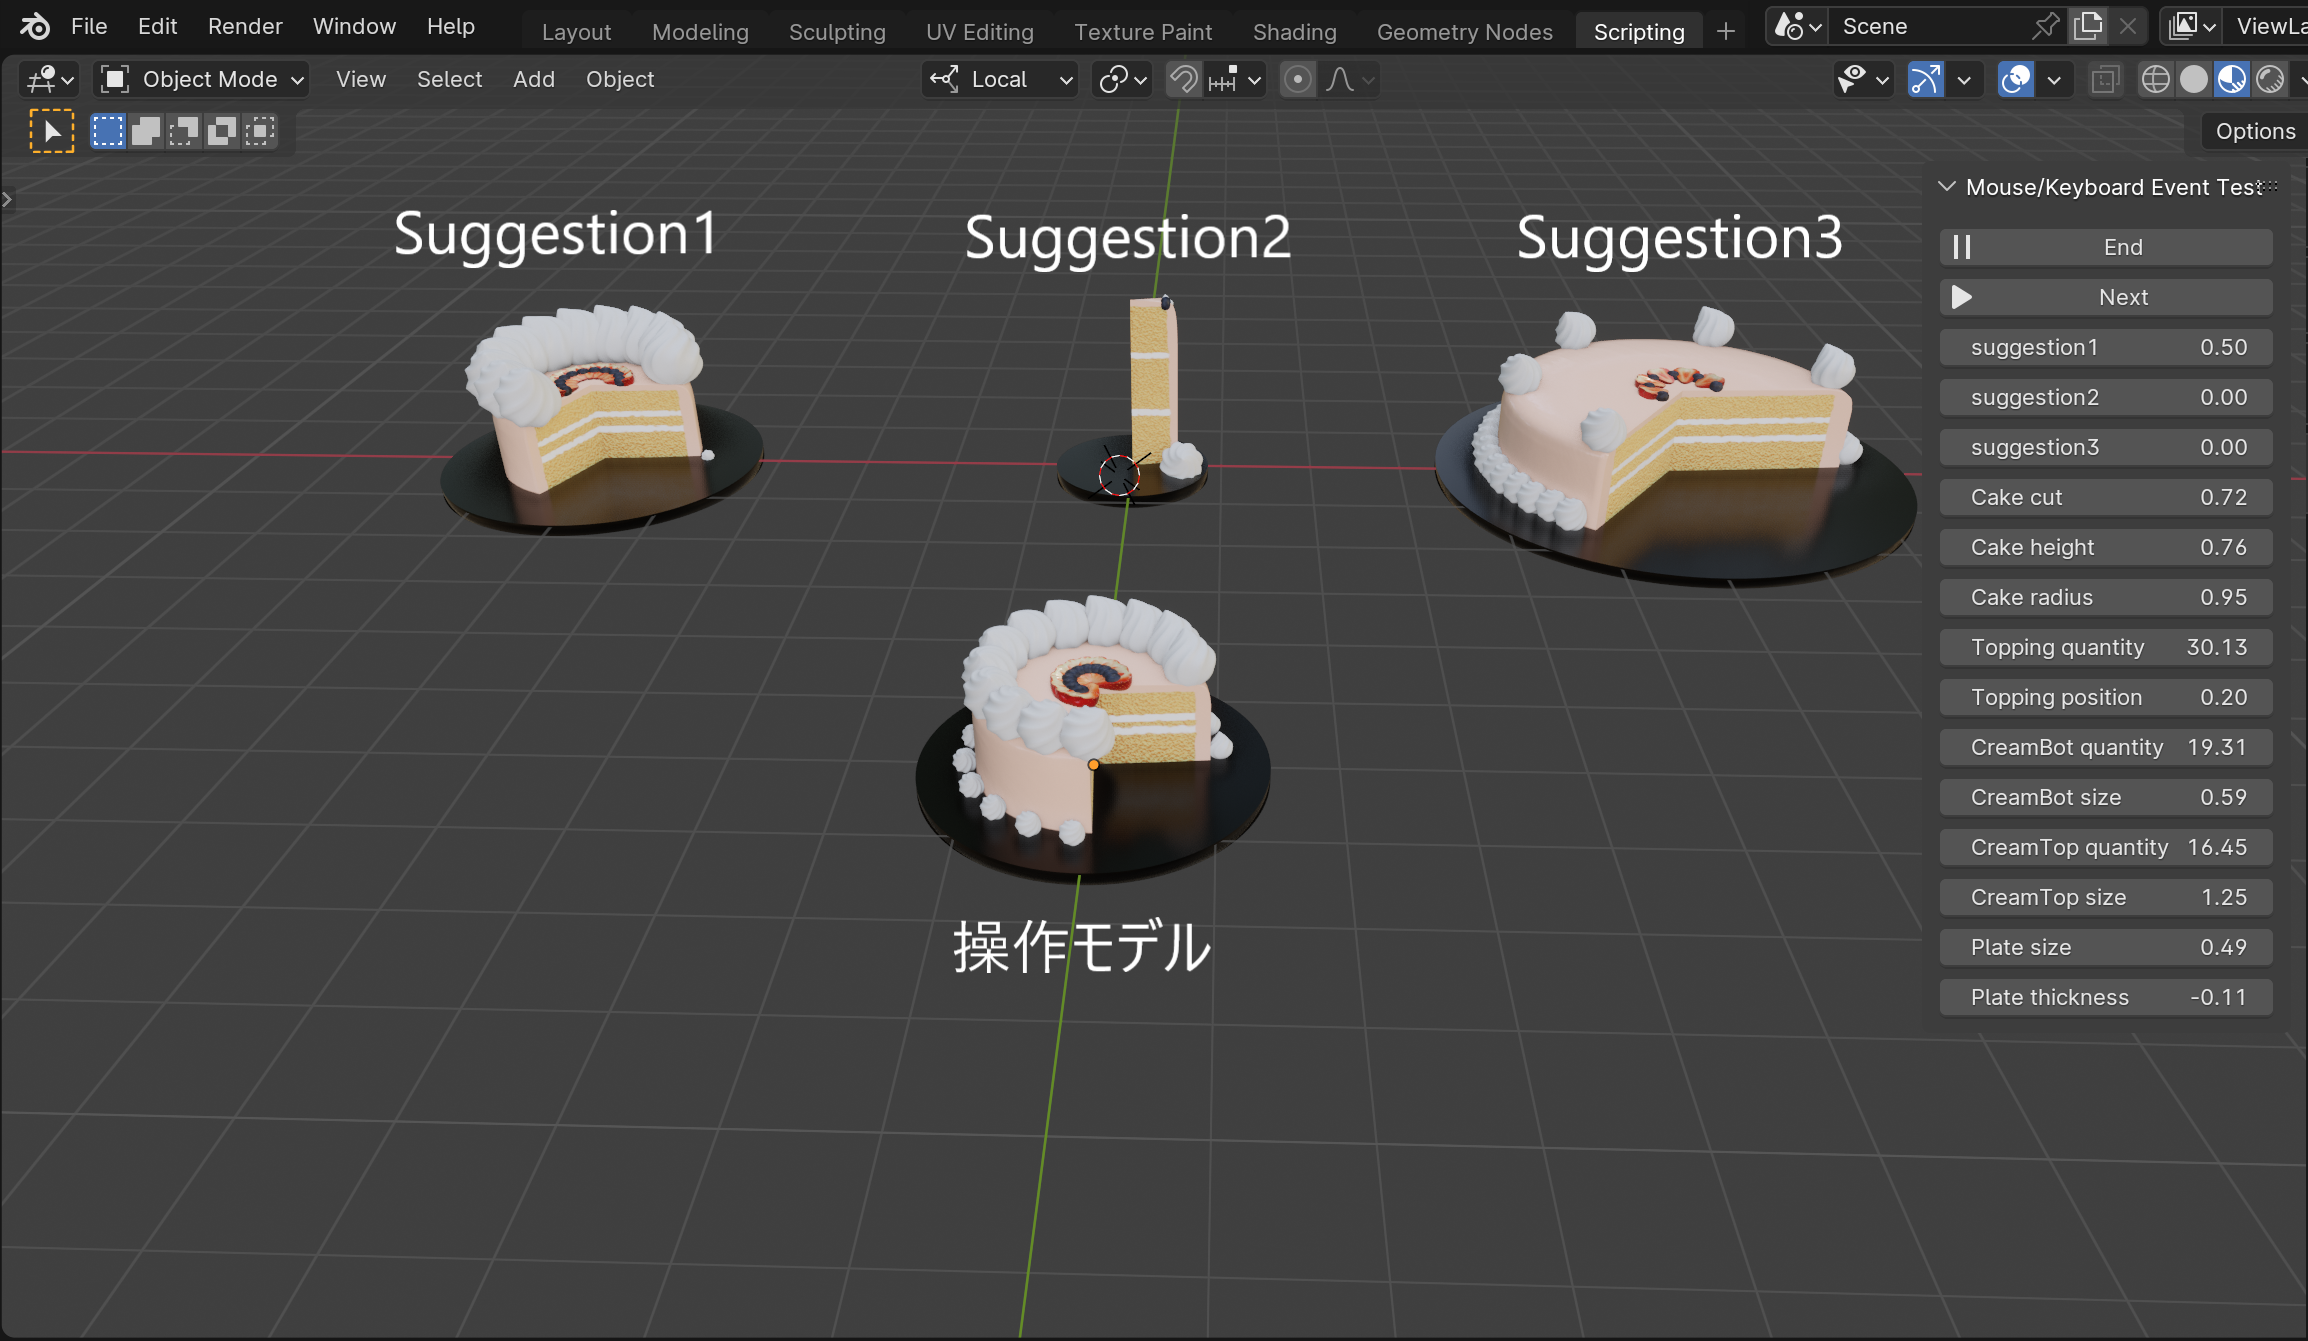
\includegraphics[scale=0.2]{./imgs/boAssistant2.png}
		\caption{BO as Assistant (Windows OSでの外観)\label{fig:boAssistant2}}
	\end{center}
\end{figure}
\newpage


\subsection{アンケート項目}
表\ref{tb:questions1},\ref{tb:questions2}に本実験で行うアンケート項目を示す.
アンケートの種類は提案システムに対する評価と,対照実験と比較した場合の評価の2種類である.
回答については5段階リッカート尺度\cite{likert1932technique}によって行う.
また選択回答に加えて,システムに関する良い点,不満点,感想についての自由記述も行う.

\begin{table}[h]
        \centering
	\caption{提案システムの使用感に関するアンケート(5段階評価)\label{tb:questions1}}
	\scalebox{1.0}{
		\begin{tabular}{|l|} \hline
                 1 : 使用方法について理解するには簡単であると感じましたか?\\ \\
                 2 : 使いやすいと感じましたか?\\ \\
                 3 : 操作時間は短いと感じましたか?\\ \\
                 4 : 操作する項目数は少ないと感じましたか?\\ \\
                 5 : モデルを広く探索できたと感じましたか?\\ \\
                 6 : 満足のいくモデリングが出来ましたか?\\ \\
                 7 : プロシージャルモデリングをするときに有用性があると感じましたか?\\ \\
                 8 : また本システムを使いたいと感じましたか?\\ \hline
		\end{tabular}
	}
\end{table}

\begin{table}[t]
        \centering
	\caption{対照実験との比較に関するアンケート(5段階評価)\label{tb:questions2}}
	\scalebox{1.0}{
		\begin{tabular}{|l|} \hline
                 9 : 目的のモデルが与えられた実験ではどちらの方が利用するのに適していると思いますか?\\ \\
                 10 : 自由にモデリングをした実験ではどちらの方が利用するのに適していると思いますか?\\ \\
                 11 : パラメータ数が少ないモデルではどちらの方が利用するのに適していると思いますか?\\ \\
                 12 : パラメータ数が多いモデルではどちらの方が利用するのに適していると思いますか?\\ \\
                 13 : モデリングにかかる時間はどちらの方が長いと感じましたか?\\ \\
                 14 : モデルの探索範囲はどちらの方が広いと感じましたか?\\ \\
                 15 :どちらのシステムが有用性が高かったですか
                 \\ \hline
		\end{tabular}
	}
\end{table}
\newpage


\subsection{実験の流れ}
本実験ではモデルのパラメータ数が実験1よりも実験2のほうが多いものを利用している関係上,実験2のタスクのほうが難度が高いものになっている.システム操作の理解が高い状態で難度の高いタスクを行ってもらうために,実験1の次に実験2を取り組みという手順で固定している.以下に,実験の順序を説明する.

\begin{enumerate}
    \item プロシージャルモデリングの簡単な説明
    \item 提案システム,対照実験用システムの説明および練習
    \item Cake モデルのパラメータ説明,動作確認
    \item 実験1
    \item Sofa モデルのパラメータ説明,動作確認
    \item 実験2
    \item アンケート回答
\end{enumerate}

\clearpage
\section{結果と考察}
\subsection{定性評価}
図\ref{fig:exp1TimeComp}にシステムの操作時間についての箱ひげ図を示す.表\ref{tb:exp1TimeComp}に各平均値,標準偏差を示す.時間の平均値に関して提案システムのほうが,既存システムよりも短縮されているようにも見えるが,図\ref{fig:exp1TimeComp}からも分かるように,既存システムでは大きな値に外れ値が存在するためであると考えられる.一方で,図\ref{fig:exp1AllTime}において提案システムのほうがばらつきが大きいことが分かる.この差について,システム理解における差ではないかと考えられる.実験の流れとして,実験の前にプロシージャルモデリングの各パラメータが何を示すのかを理解するために一度パラメータ操作をしてもらっており,既存システムではパラメータ操作に追加機能を実装する形のものである.そのため,システム操作の理解度が提案システムのほうが低かったために生じた差であると考えられる.


また,1ステップごとの提案モデルおよび決定したモデルの見本のモデルへの推移について,具体的なグラフは\hyperref[appendix:gaChange]{付録B}にて掲載する.結果として,システムが機能し収束していくデータもあれば,上手くいかないものもあった.これは IGA のランダム性の高さが寄与していると考えられる.



\begin{figure}[h]
 \begin{minipage}[b]{0.48\linewidth}
  \centering
  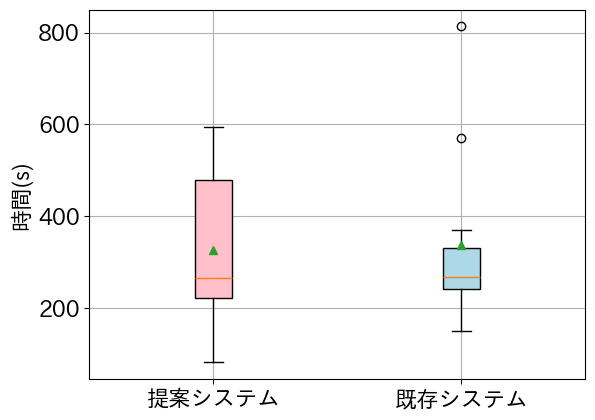
\includegraphics[scale=0.4]{./imgs/result/cakeAllTime.png}
        \subcaption{全時間}\label{fig:exp1AllTime}
 \end{minipage}
 \begin{minipage}[b]{0.48\linewidth}
  \centering
  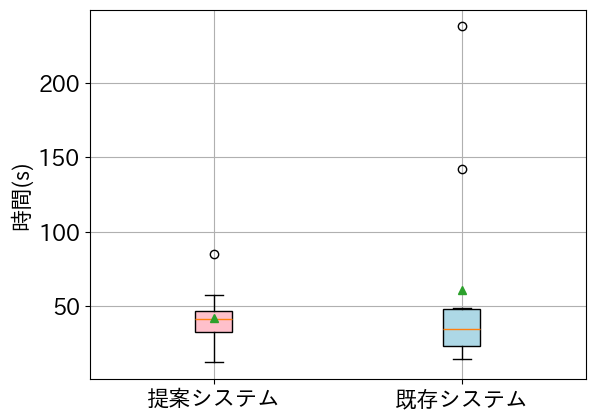
\includegraphics[scale=0.4]{./imgs/result/cakeStepTime.png}
        \subcaption{1ステップ当たりの時間}
 \end{minipage}\\
 \begin{minipage}[b]{0.48\linewidth}
  \centering
  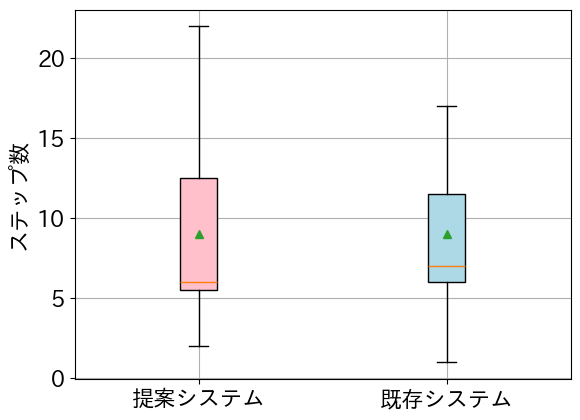
\includegraphics[scale=0.4]{./imgs/result/cakeStepCnt.png}
        \subcaption{ステップ数}
 \end{minipage}
 \caption{実験1における操作時間の比較}\label{fig:exp1TimeComp}
\end{figure}

\begin{table}[h]
	\centering
	\caption{実験1における操作時間の平均と標準偏差\label{tb:exp1TimeComp}}
		\begin{tabular}{|c|c|c|c|} \hline
                システム&&平均&標準偏差\\ \hline\hline
                \multirow{3}{*}{既存システム}&全時間&337.445 s&181.72 s \\ \cline{2-4}
                &1ステップ当たりの時間&61.004 s&65.144 s \\ \cline{2-4}
                &ステップ数&9.0000 回&4.8617 回 \\ \hline
                \multirow{3}{*}{提案システム}&全時間&326.39 s&171.22 s \\ \cline{2-4}
                &1ステップ当たりの時間&42.079 s&17.804 s \\ \cline{2-4}
                &ステップ数&9.0000 回&5.7525 回 \\ \hline
		\end{tabular}
\end{table}
\newpage

図\ref{fig:exp2TimeComp}にシステムの操作時間についての箱ひげ図を示す.表\ref{tb:exp2TimeComp}に各平均値,標準偏差を示す.図\label{fig:exp2AllTime}について,実験1よりも速い時間で終わっている.この原因としてはシステム操作への慣れと,実験1の終了判定の曖昧さの二つが考えられる.実験1の終了判定の曖昧さについて,終了基準は被験者本人の判断に任せているため,人によってはかなり厳密な調整を行っていた.一方で実験2でも終了条件自体は本人の基準ではあるが,実験1と違い見本画像がないため,より甘い基準で終了することが出来たためであると考えられる.

実験1同様に,1ステップごとの提案モデルおよび決定したモデルの見本のモデルへの推移について,具体的なグラフは\hyperref[appendix:gaChange]{付録B}にて掲載する.結果について,実験1とは反し,ランダム性によってステップ数が比較的短く終了したケースが多く存在する.一方で本システムとしては,4ステップで GA における一世代分に相当しているので GA としての収束機能が働かずに終わったということでもある.

\begin{figure}[h]
 \begin{minipage}[b]{0.48\linewidth}
  \centering
  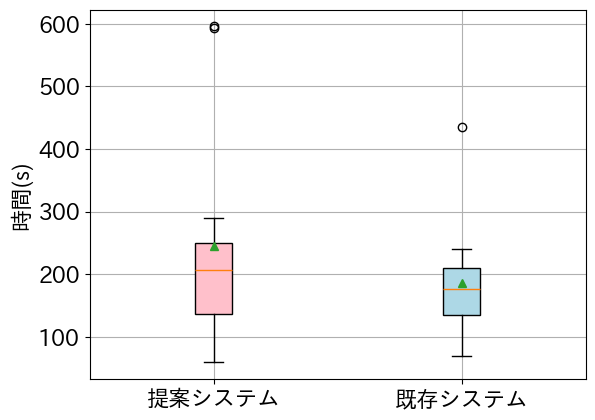
\includegraphics[scale=0.4]{./imgs/result/sofaAllTime.png}
        \subcaption{全時間}\label{fig:exp2AllTime}
 \end{minipage}
 \begin{minipage}[b]{0.48\linewidth}
  \centering
  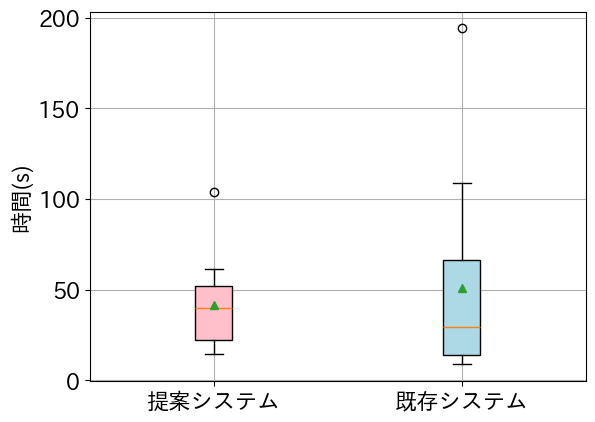
\includegraphics[scale=0.4]{./imgs/result/sofaStepTime.png}
        \subcaption{1ステップ当たりの時間}
 \end{minipage}\\
 \begin{minipage}[b]{0.48\linewidth}
  \centering
  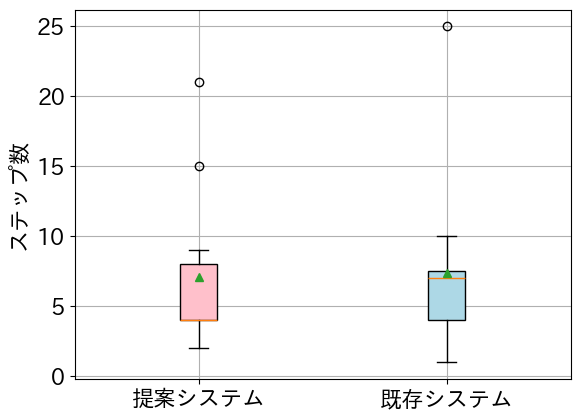
\includegraphics[scale=0.4]{./imgs/result/sofaStepCnt.png}
        \subcaption{ステップ数}
 \end{minipage}
 \caption{実験2における操作時間の比較}\label{fig:exp2TimeComp}
\end{figure}

\begin{table}[h]
	\centering
	\caption{実験2における操作時間の平均と標準偏差\label{tb:exp2TimeComp}}
		\begin{tabular}{|c|c|c|c|} \hline
                システム&&平均&標準偏差\\ \hline\hline
                \multirow{3}{*}{既存システム}&全時間&186.45 s&93.881 s \\ \cline{2-4}
                &1ステップ当たりの時間&51.136 s&56.049 s \\ \cline{2-4}
                &ステップ数&7.3636 回&6.1241 回 \\ \hline
                \multirow{3}{*}{提案システム}&全時間&245.70 s&175.30 s \\ \cline{2-4}
                &1ステップ当たりの時間&41.658 s&24.727 s \\ \cline{2-4}
                &ステップ数&7.0909 回&5.5996 回 \\ \hline
		\end{tabular}
\end{table}
\newpage


ここで表\ref{tb:paramTimeComp}に全体の操作時間のうち,個別のパラメータ調整をしている時間の比率を示す.
実験2の提案システムのものでは個別のパラメータ操作時間が非常に短いことが分かる.これは,個別パラメータを触らなかった被験者が8人いたからであり,明確な目的を持たずに動かす場合は提案システムの有効性が顕著であると考えられる.一方で既存システムでは全ての被験者が触れていた.これは既存システムのベイズ最適化の関係上,モデルに必要であると考えるパラメータを大きく動かさなければモデルの提案が滞ることと,常に操作できる位置に表示されていることが原因であると考えられる.
\begin{table}[h]
	\centering
	\caption{操作時間比率の平均と標準偏差\label{tb:paramTimeComp}}
		\begin{tabular}{|c|c|c|c|} \hline
                実験&システム&平均&標準偏差\\ \hline\hline
                \multirow{2}{*}{実験1}&既存システム&0.33493&0.14318 \\ \cline{2-4}
                &提案システム&0.24657& 0.17479 \\ \hline
                \multirow{2}{*}{実験2}&既存システム&0.41585&0.21003 \\ \cline{2-4}
                &提案システム&0.04111&0.07231 \\ \hline
		\end{tabular}
\end{table}
\newpage

その中で,図\ref{fig:tSNE_example}に t-SNE\cite{van2008visualizing} を用いてある被験者がシステムによって提案された Sofa モデルのパラメータを次元削減し可視化したものの一例を示す.全ての可視化図は\hyperref[appendix:tSNE]{付録C}に掲載する.
この散布図について縁取りが青いものが提案システム,赤いものが既存システムによる提案モデルであり,内部の色が0から1に行くにつれてステップ数が増加するようにしている.


提案システムのほうが既存システムの二倍のモデル提案を行うためプロット数自体は多い傾向にあるが,提案システムのほうがより広範囲の探索を行えているように見える.特に,既存システムにおいてより後のステップのもの同士が非常に近い位置にプロットされているのが確認できる.これはベイズ最適化によるモデル提案について,次の提案を行う直前に決定したモデルがそれまでに決定したモデルと大きく違うパラメータがあればそれをより再現しようとする方向に作用するためであり,収束率が高い一方でステップ数が大きくなるにつれ極端に探索範囲が狭まることに起因する.一方で提案システムのほうは多親交叉 REX によるランダム性があるため,ステップ間で見れば範囲は狭くなっているものの,多様性の保持が見られる.

\begin{figure}[h]
	\begin{center}
		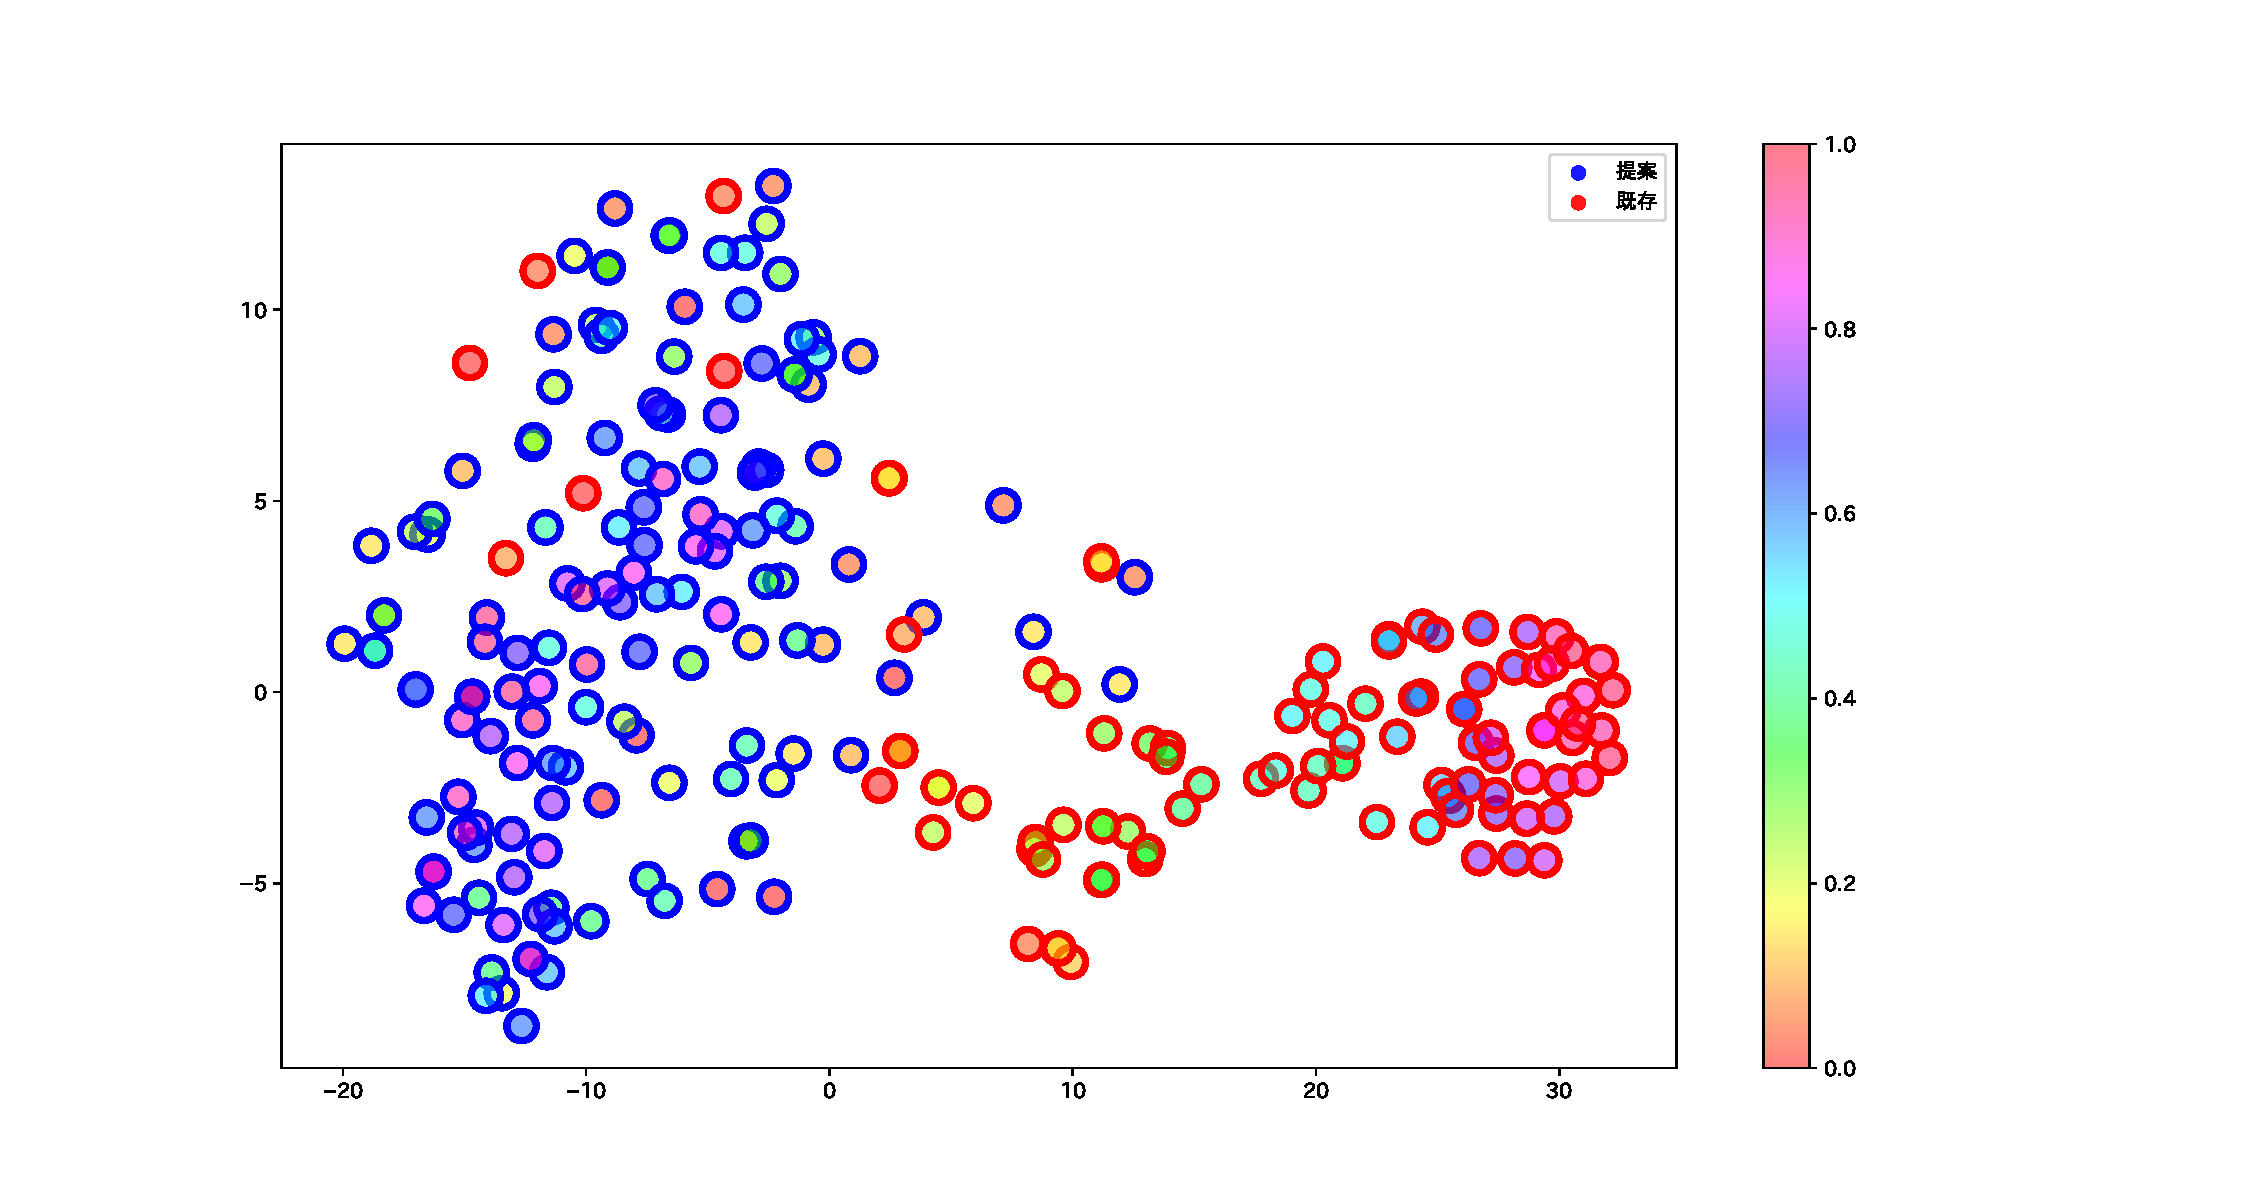
\includegraphics[scale=0.35]{./imgs/tSNE/sofa_5.pdf}
		\caption{提案された Sofa モデルのパラメータを二次元可視化した一例\label{fig:tSNE_example}}
	\end{center}
\end{figure}

\clearpage
\subsection{アンケート}

\subsubsection{選択}
図\ref{fig:questAns1},\ref{fig:questAns2}にアンケート結果を示す.図\ref{fig:questAns1}では1が negative, 5が positiveな評価であり,図\ref{fig:questAns2}では1が既存システム,5が提案システム寄りであることを示す.

まず提案システムの使用感について,全ての回答で平均が3を超えており,特にQ5-Q8については全て4を超えている.このことからシステム UI の方向性は間違っていないと考えられる.しかし,Q1の意見では良し悪しが分かれており,これは,ドラッグ操作と選択操作二種類がある点や,画面上に存在するモデルが計10個もあるという点によって分かりづらさがあったのではないかと考えられる.

次に対照実験との比較について,提案システムの優勢が高いと感じられたのはQ10,Q12,Q14であり,自由なモデリング,パラメータ数が多い時,探索範囲を広くしたい時にユーザの評価が高い.一方で,パラメータ数が少ないモデリング,操作時間については既存システムのほうが評価が高い.このことから,本システムはより複雑性の高いタスクに有効であり,簡単なモデリングであれば既存システムのほうが良い可能性がある.

\begin{figure}[h]
	\begin{center}
		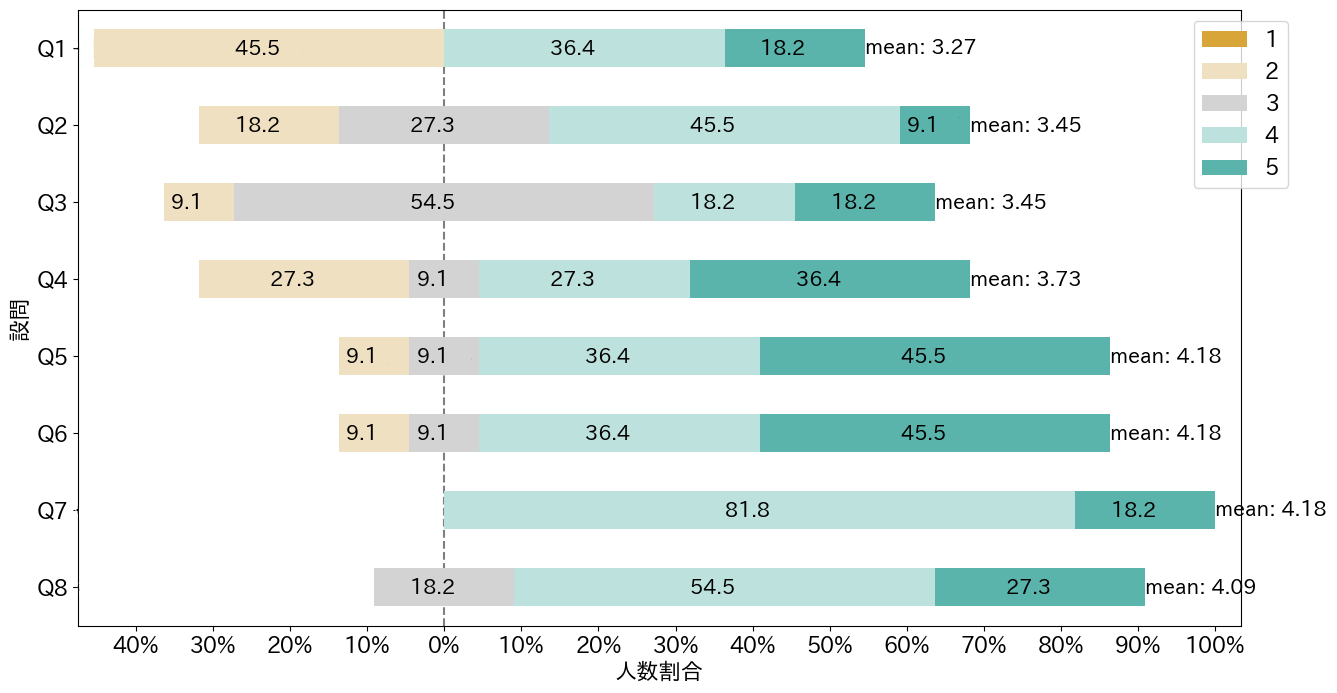
\includegraphics[scale=0.35]{./imgs/answer/questAns1.png}
		\caption{提案システムの使用感に関するアンケート結果\label{fig:questAns1}}
	\end{center}
\end{figure}

\begin{figure}[h]
	\begin{center}
		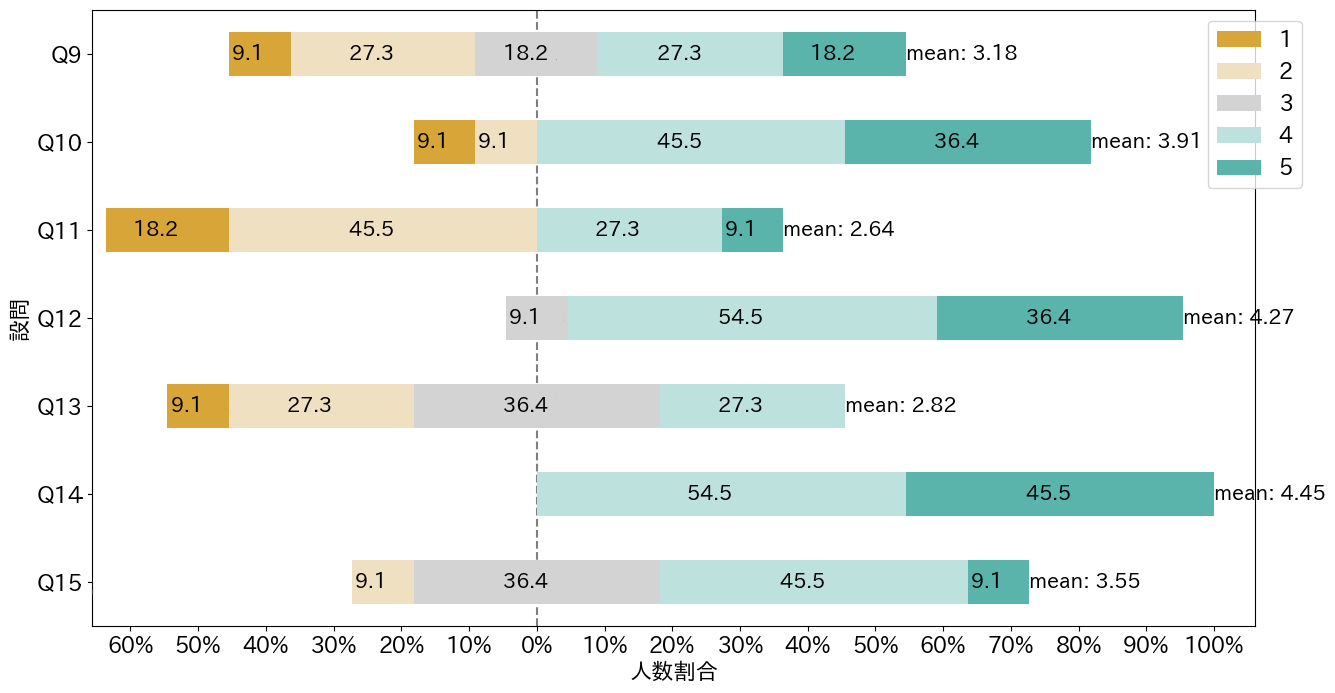
\includegraphics[scale=0.35]{./imgs/answer/questAns2.png}
		\caption{対照実験との比較に関するアンケート結果\label{fig:questAns2}}
	\end{center}
\end{figure}

\clearpage
\subsubsection{自由記述}
自由記述の回答について以下に示す.



\textbf{\underline{システムの良い点}}
\begin{enumerate}\label{en:systemGood}
    \item 新しいシステムは使いこなせれば大雑把に決めて、細かい部分だけ調整すれば完成できるため時間短縮になると感じました
    \item ソファでいう手すりの部分が欲しいというような理想を簡単にサイクルを回すことで再現することができる点が良いと思った。
    \item 自由にモデリングするパターンでは、パラメータの調整が直感的だった。
    \item 三角形の UI は直感的でわかりやすいとおもった
    \item 直感的で理解しやすかった.自由にモデリングをする実験では,自分が思いもよらないモデルができて良かったし,楽しかった.このシステムはパラメータが多くなるほど有用性が高まるように感じる.
    \item パラメータを動かしたときにモデルができるいろいろなパターンを先に見れることで、想像力が掻き立てられた
    \item 思いもよらないものができてくる点。とりあえず動かしてみて遊ぶことができる点。
    \item パラメータをが多いモデルはどれがどんな役割を持つのか把握しずらいため、ドラッグ操作のみで様々なモデルを探索できるのがとてもよかった。
    \item パラメータ調整でモデリングできたのはよかった
    \item 細かい操作をしなくても、システムがリコメンドしてくれて、形がそれっぽくなるのが楽だった
\end{enumerate}





\textbf{\underline{システムの悪い点}}
\begin{enumerate}
    \item 三角形の角に合わせて選択するやつが、左角から順番に選ばないといけないのが直感的には使いにくかったです
    \item 凝り性の人は、かなり時間がかかるかもしれないと感じた
    \item 赤い点の判定がもう少し広い方がよかったです。欲しいパーツが出てこないことがあり、直接パラメータを調整しなければいけない場合があった。
    \item 1個(例えばクリームの見た目)について近づけようとモデルを選んでいるといつの間にか他のが全然違くなっていることがあって難しいと感じた
    \item 最終的にディテールを突き詰める部分は,パラメータを調整する必要があると感じた.
    \item 目標が明確な時に、それから遠ざかるような選択肢しかない時がもどかしい
    \item 最初に選んだ三つのモデルから良いなと思ったモデルができたとき、次に新しい三つを選ぶとそれが消えてしまった。前段階で作成したモデル+新しい提案との組み合わせができるとよいなと思いました
    \item 最初に提案されるモデルの方向性を指定できると更に楽だと思いました
\end{enumerate}





\textbf{\underline{システムのその他感想}}
\begin{enumerate}
    \item 三角形の操作について理解するのに時間がかかった
    \item 時間制限が設けてある場合に使用するとかなり効果があるシステムだと感じた
    \item 大雑把な調整(概形)を提案システムで行って、細かい調整ができないパラメータ(整数のやつ)を最後に仕上げでいじるのが使いやすいのかなと思った
    \item 大雑把に形を作る際は,提案システムを利用することで,既存システムを利用するよりも早く完成させることができると感じた.
    \item 携帯のアプリケーションにしたら面白そう
    \item 後半になればなるほど、ここだけピンポイントで直したいということが多い
    \item 趣味で 3D モデリングをたしなんでいますが、システムから提案された複数のモデルを組み合わせる手法は、自身の発想からはみ出したアイデアを作品に組み込むことができてとても面白いなと思いました。
    \item 実用性は無いかもしれませんが、もっと色々なものが候補に出て、混ぜるとそれっぽくなるのは見てみたいです
    \item ランダムセレクトの因子が欲しかった。3要素のうちひとつめは、現在の最新モデルに固定してもよかったと思う(それまでの作業がキャンセルされてしまうため)
\end{enumerate}


システムの良い点としては UI の補間操作でドラッグによる直感的である点と,パラメータを同時に動かせることによって広く,おおまかな探索が出来る点が評価された.反対に悪い点としては,UIの操作性の悪さと,IGAによるランダム性が悪い方向に作用してユーザが良くないと思う方向へのモデル提案が行われてしまった点,細かい調整が提案システムだけでは難しい点が挙げられた.

\clearpage
\subsection{評価結果まとめ}
提案システムとしては,提案のランダム性および平面UIによる補間システムによって非常に幅広い探索が出来るシステムになったことが確かめられた.その一方で,本来の目的としていた時間短縮に関しては既存システムに対して優位性が見られなかった.ただし,ステップ数および操作時間に関して同等程度の結果である反面,広い探索を行えたという点に注目すれば探索についてのユーザビリティ向上は行えたと考えられる.

多くのパラメータを持つモデリングでは個別にパラメータが動かせる状況であれば,それに頼ることが多くなる.その結果Q12にみられるようにパラメータの多いモデリングでは提案システムに高い有効性があると考えられる.以上から,提案システムにおける UI は操作時間こそ減らすことは出来なかったものの,プロシージャルモデリングにおいて有効性が高いと考えられる.


一方で,遺伝的アルゴリズムによるモデル提案については上手く機能していると言い難く,実験2のように明確な目的がなければ,現状の UI だけで事足りてしまうことが多かった.そのため,明確な目的があれば収束する方向に,そうでなければ現在の操作モデルから大きく離れたモデルを提案する事でよりモデリング時の新しい発想が生まれて,洗練されたモデリングになっていくのではと考えられる.
\clearpage

\newpage

\chapter{おわりに}

\section{結論}
本研究ではプロシージャルモデリングにおける操作性およびモデリング時間の改善のため,インタラクティブ遺伝的アルゴリズムにおけるモデル提案と,平面 UI による補間を用いたモデリング支援システムを提案した.従来のパラメータを個別で動かすのではなく,モデルの補間という形でパラメータ群を同時に操作するとともに,平面 UI によって3つのモデルから補間されることにより直感的な操作で広い空間の探索を行うことが可能になった.ユーザスタディの結果,定量評価では既存手法に比べ時間的優位性を見出すことはできなかったが,定性評価から,自由かつ多くのパラメータが存在するときには有用性は確認できた.一方でインタラクティブ遺伝的アルゴリズムの有効性を確認することはできなかった.
\section{今後の課題}
課題点は大きく2点あり,他のプロシージャルモデリングへの対応とモデル提案手法の検討である.今回は2種類のモデルを用いたが,さらに多くのパラメータを持つ場合や,ストロークによって入力が行われるもの,あるいは物理演算やアニメーションといった様々なものへの応用の検討が考えられる.またモデル提案手法の改善として,本研究で用いた IGA では有用性が確認できなかったため,高次元への対応をしたベイズ最適化\cite{平沼智之2021組合せ最適化におけるベイジアン最適化アルゴリズムを組み込んだ遺伝的アルゴリズムの提案}や機械学習といった方法によって,効率的なモデル提案を行う事が出来ればより高速なモデリングに繋がると考えられる.
\clearpage

\newpage

\chapter*{謝辞}
\addcontentsline{toc}{chapter}{謝辞}


本研究を進めるにあたりご指導,ご鞭撻を賜りました宮田一乘教授に深く感謝申し上げます.
また,実験協力や発表スライドや本論文の作成にあたり添削及びアドバイスを下さった宮田研究室の皆様にも厚く御礼を申し上げ,
感謝の意を表します.
\begin{flushright}
	2024年1月26日
\end{flushright}


\clearpage



%% reference
\clearpage
%\include{./doc/bibliography}
%\bibliographystyle{unsrt}
\bibliographystyle{unsrt}
\bibliography{reference}


\clearpage
\appendix

\def\thesection{付録\Alph{section}}
\renewcommand{\thetable}{\Alph{section}.\arabic{table}}
\renewcommand{\thefigure}{\Alph{section}.\arabic{figure}}


\section{使用したモデルのパラメータの意味}\label{paramMean}
本付録では,使用したモデルのパラメータの意味について名前としてある程度整備されているが,実際の入力でどのように変化するのかを示す.
図\ref{fig:cakeParamMean_1} - \ref{fig:cakeParamMean_4}に
Cake モデルにおいての,図\ref{fig:sofaParamMean_1} - \ref{fig:sofaParamMean_7}に Sofa モデルにおいてのパラメータが最小と最大の時のモデルを示す.

\begin{figure}[h]
 \begin{minipage}[b]{0.48\linewidth}
  \centering
  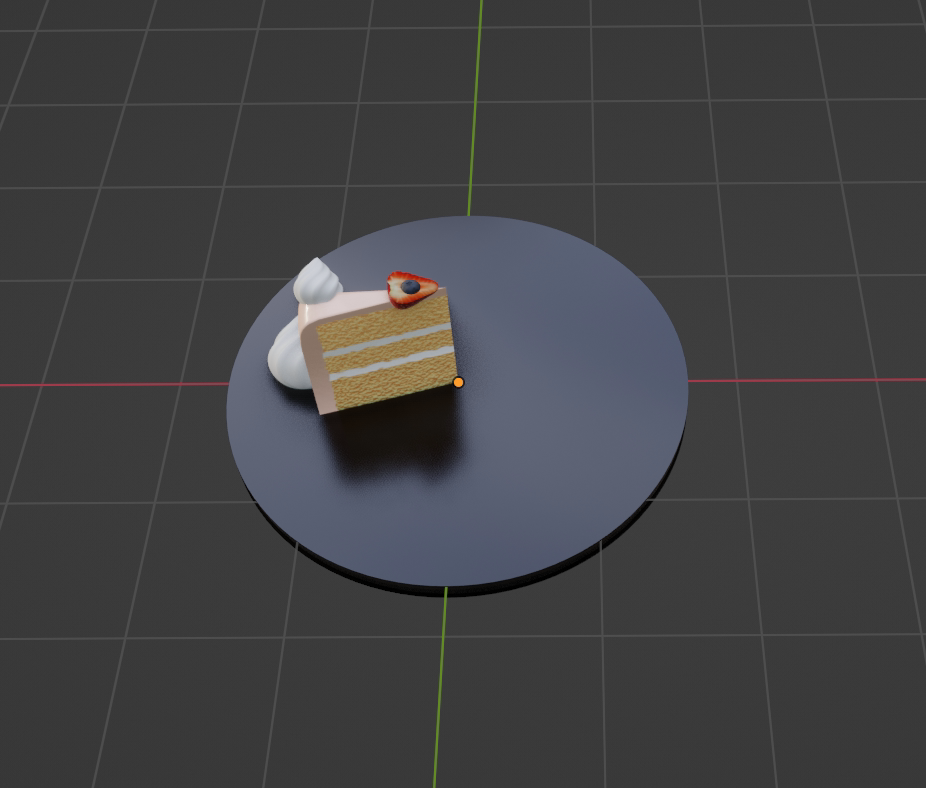
\includegraphics[scale=0.25]{./imgs/cakeParamMean/cutMin.png}
        \subcaption{Cake cut 最小(0.0)}
 \end{minipage}
 \begin{minipage}[b]{0.48\linewidth}
  \centering
  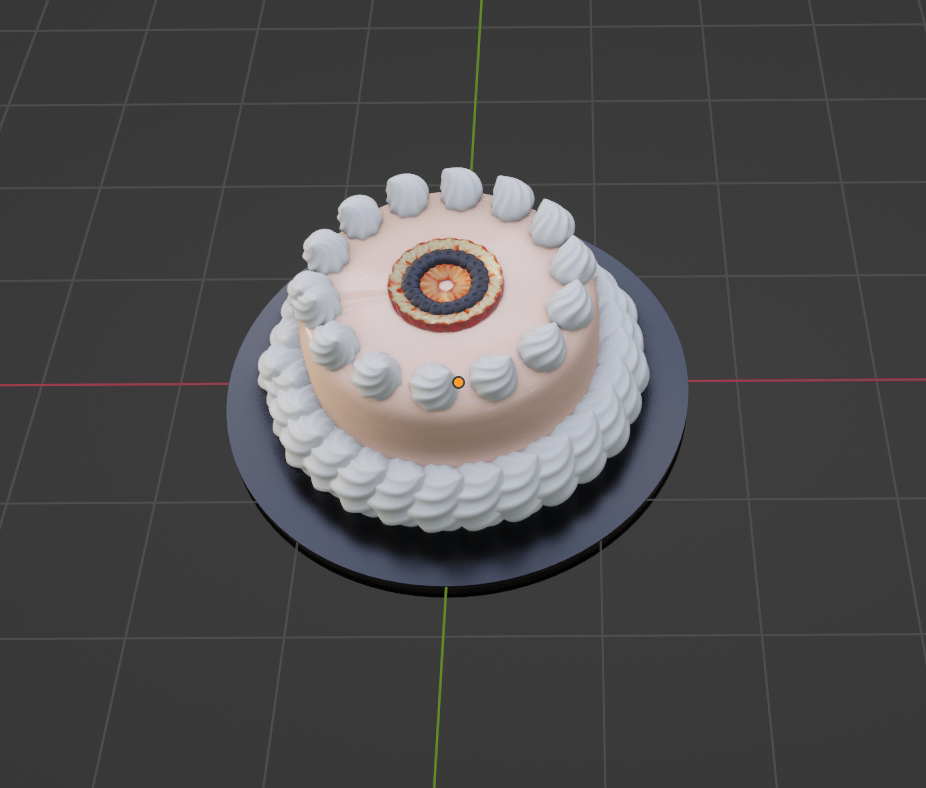
\includegraphics[scale=0.25]{./imgs/cakeParamMean/cutMax.png}
        \subcaption{Cake cut 最大(1.0)}
 \end{minipage}\\
 \begin{minipage}[b]{0.48\linewidth}
  \centering
  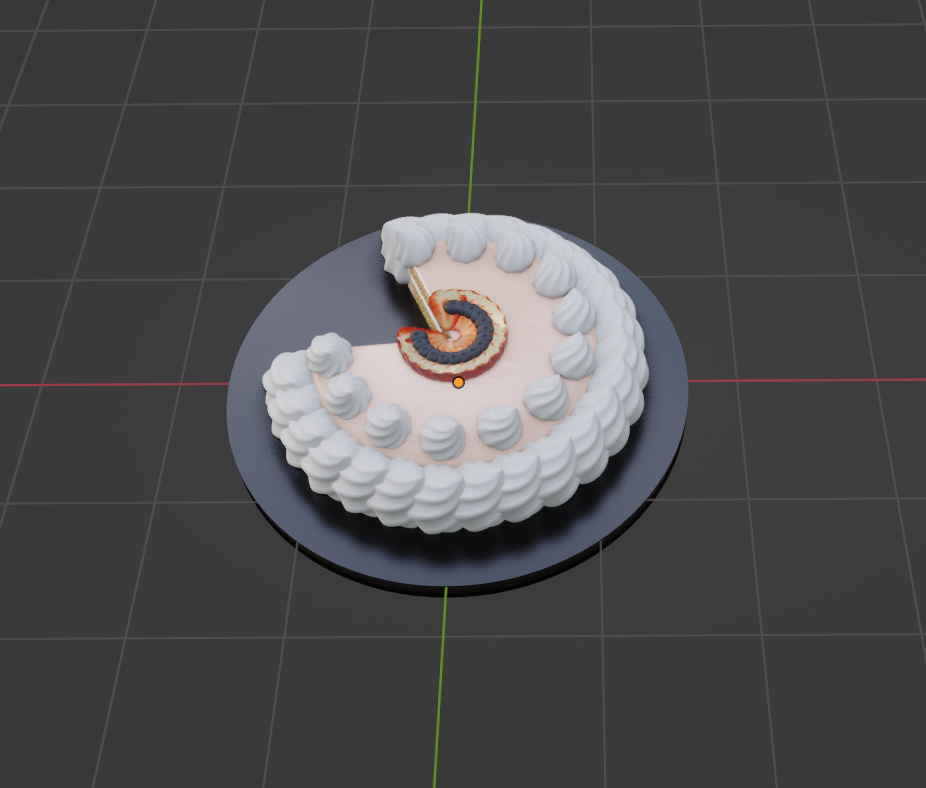
\includegraphics[scale=0.25]{./imgs/cakeParamMean/heightMin.png}
        \subcaption{Cake height 最小(0.5)}
 \end{minipage}
 \begin{minipage}[b]{0.48\linewidth}
  \centering
  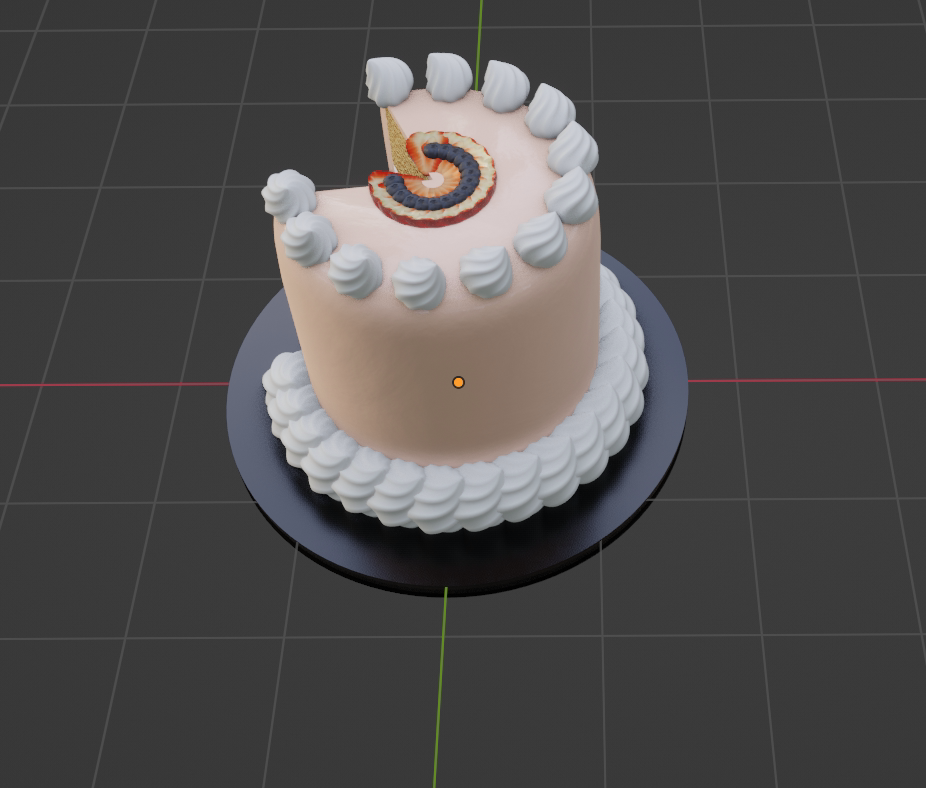
\includegraphics[scale=0.25]{./imgs/cakeParamMean/heightMax.png}
        \subcaption{Cake height 最大(2.0)}
 \end{minipage}
 \caption{Cake モデルにおけるパラメータ範囲(1)}\label{fig:cakeParamMean_1}
\end{figure}

\begin{figure}[h]
 \begin{minipage}[b]{0.48\linewidth}
  \centering
  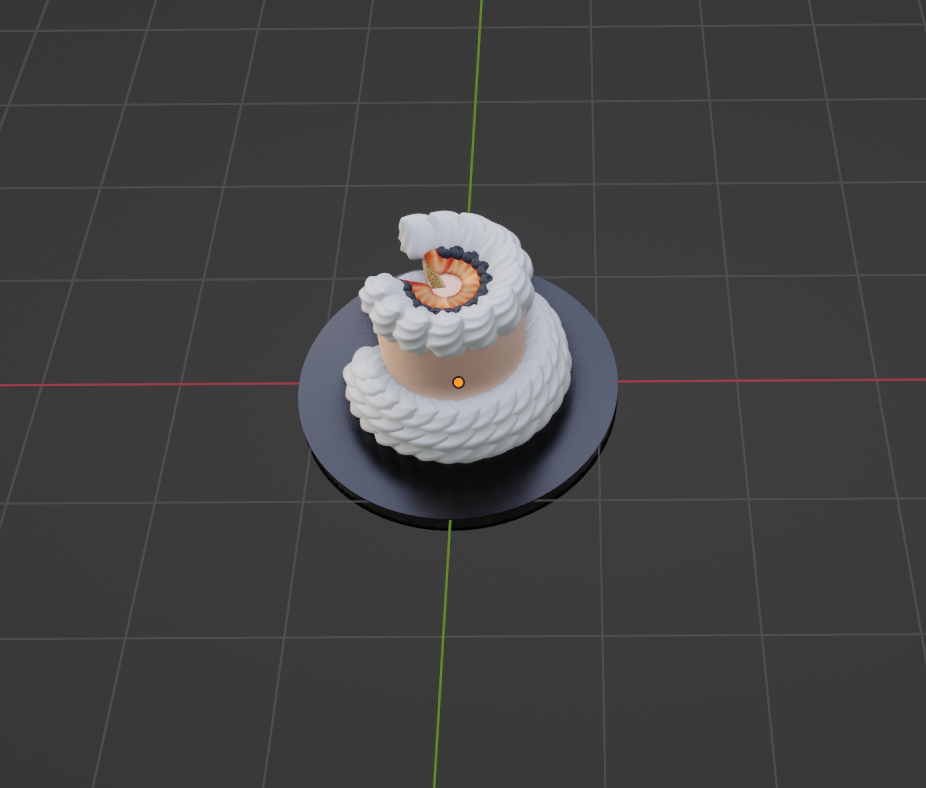
\includegraphics[scale=0.25]{./imgs/cakeParamMean/radiusMin.png}
        \subcaption{Cake radius 最小(0.0)}
 \end{minipage}
 \begin{minipage}[b]{0.48\linewidth}
  \centering
  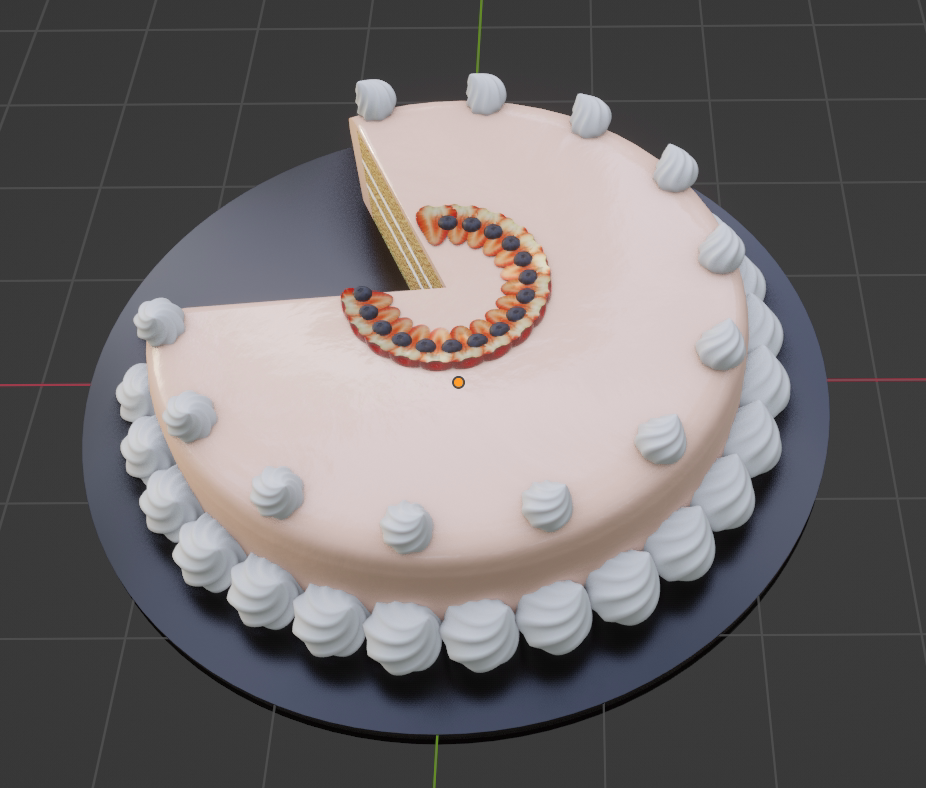
\includegraphics[scale=0.25]{./imgs/cakeParamMean/radiusMax.png}
        \subcaption{Cake radius 最大(1.0)}
 \end{minipage}\\
  \begin{minipage}[b]{0.48\linewidth}
  \centering
  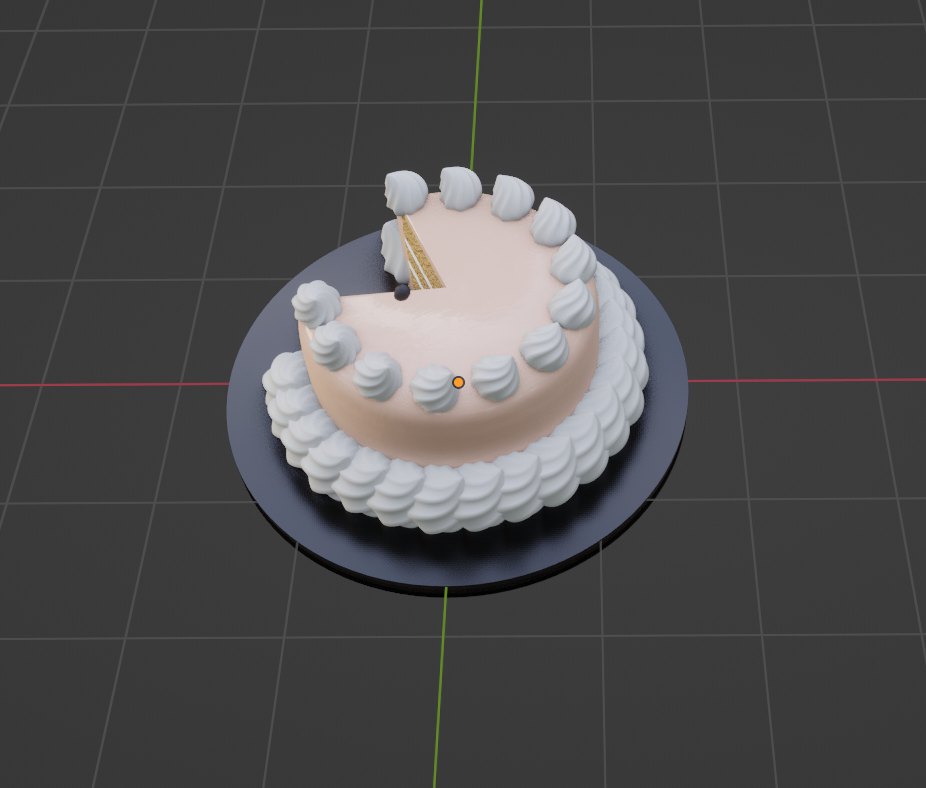
\includegraphics[scale=0.25]{./imgs/cakeParamMean/toppingQuanMin.png}
        \subcaption{Topping quantity 最小(0.0)}
 \end{minipage}
 \begin{minipage}[b]{0.48\linewidth}
  \centering
  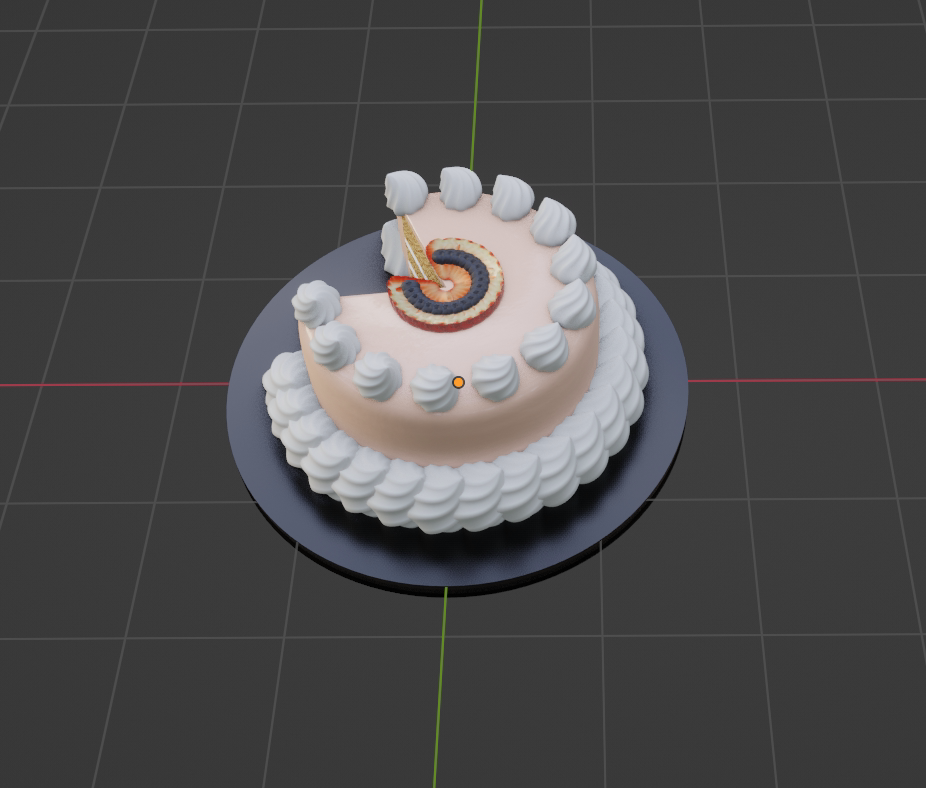
\includegraphics[scale=0.25]{./imgs/cakeParamMean/toppingQuanMax.png}
        \subcaption{Topping quantity 最大(50.0)}
 \end{minipage}\\
 \begin{minipage}[b]{0.48\linewidth}
  \centering
  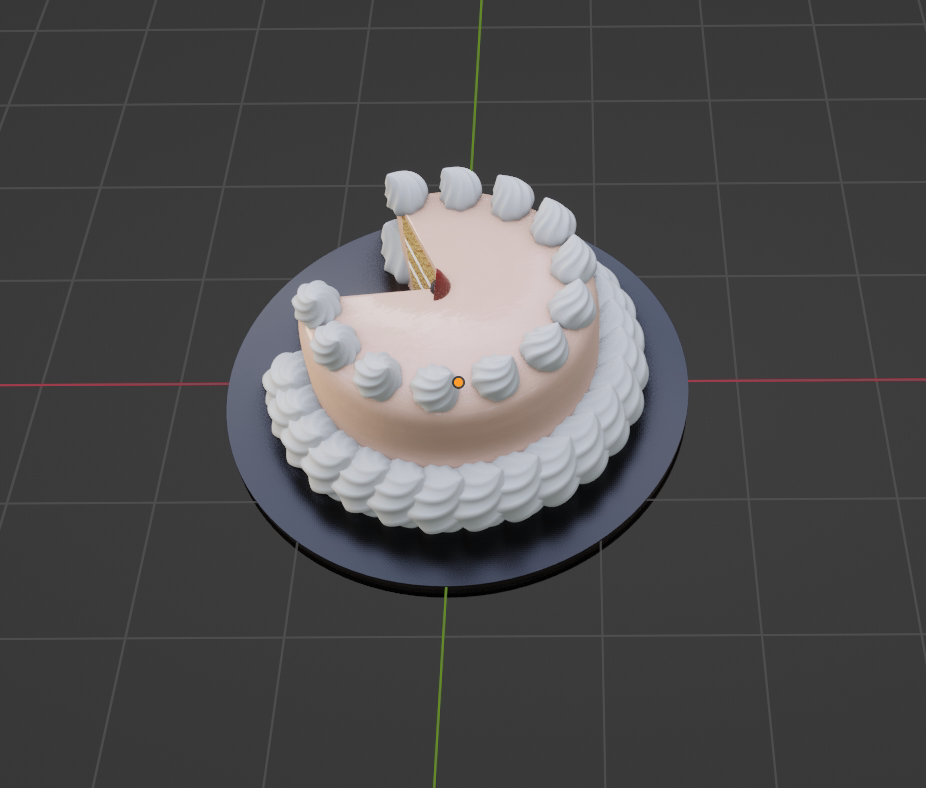
\includegraphics[scale=0.25]{./imgs/cakeParamMean/toppingPosMin.png}
        \subcaption{Topping position 最小(0.0)}
 \end{minipage}
 \begin{minipage}[b]{0.48\linewidth}
  \centering
  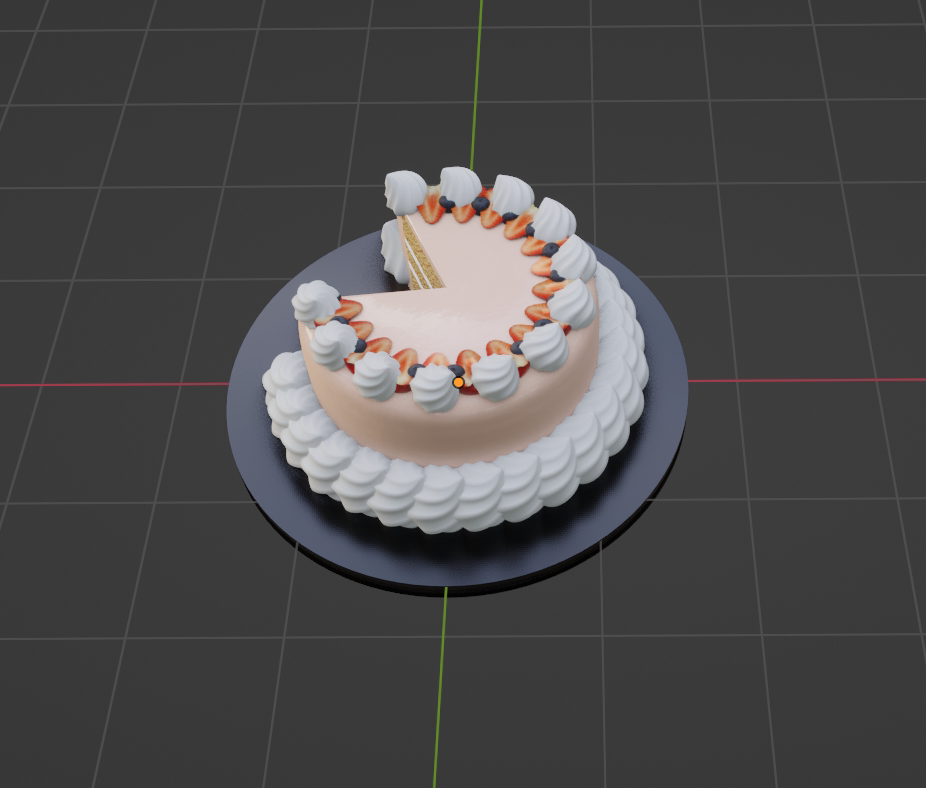
\includegraphics[scale=0.25]{./imgs/cakeParamMean/toppingPosMax.png}
        \subcaption{Topping position 最大(1.0)}
 \end{minipage}
 \caption{Cake モデルにおけるパラメータ範囲(2)}\label{fig:cakeParamMean_2}
\end{figure}

\begin{figure}[h]
 \begin{minipage}[b]{0.48\linewidth}
  \centering
  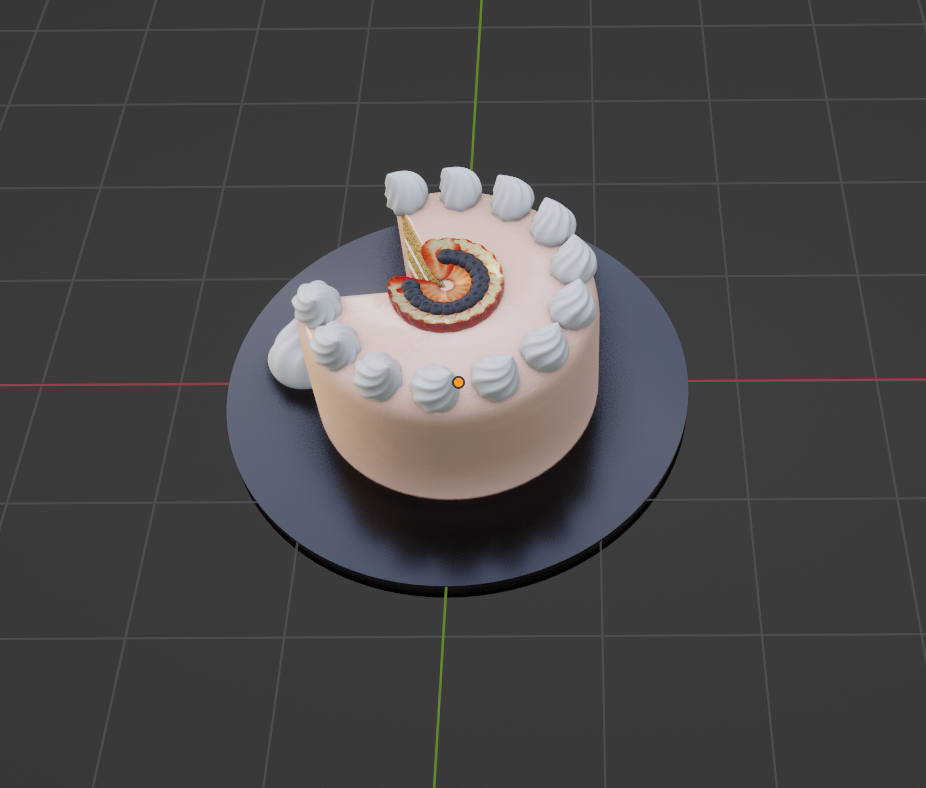
\includegraphics[scale=0.25]{./imgs/cakeParamMean/botQuanMin.png}
        \subcaption{CreamBot quantity 最小(0.0)}
 \end{minipage}
 \begin{minipage}[b]{0.48\linewidth}
  \centering
  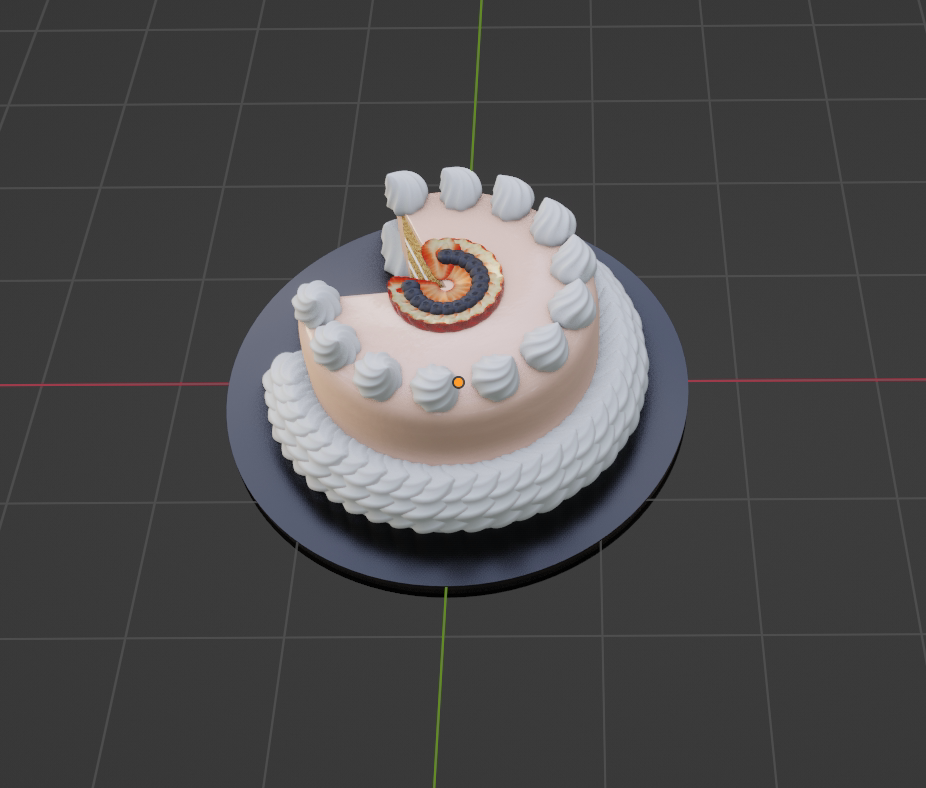
\includegraphics[scale=0.25]{./imgs/cakeParamMean/botQuanMax.png}
        \subcaption{CreamBot quantity 最大(50.0)}
 \end{minipage}\\
  \begin{minipage}[b]{0.48\linewidth}
  \centering
  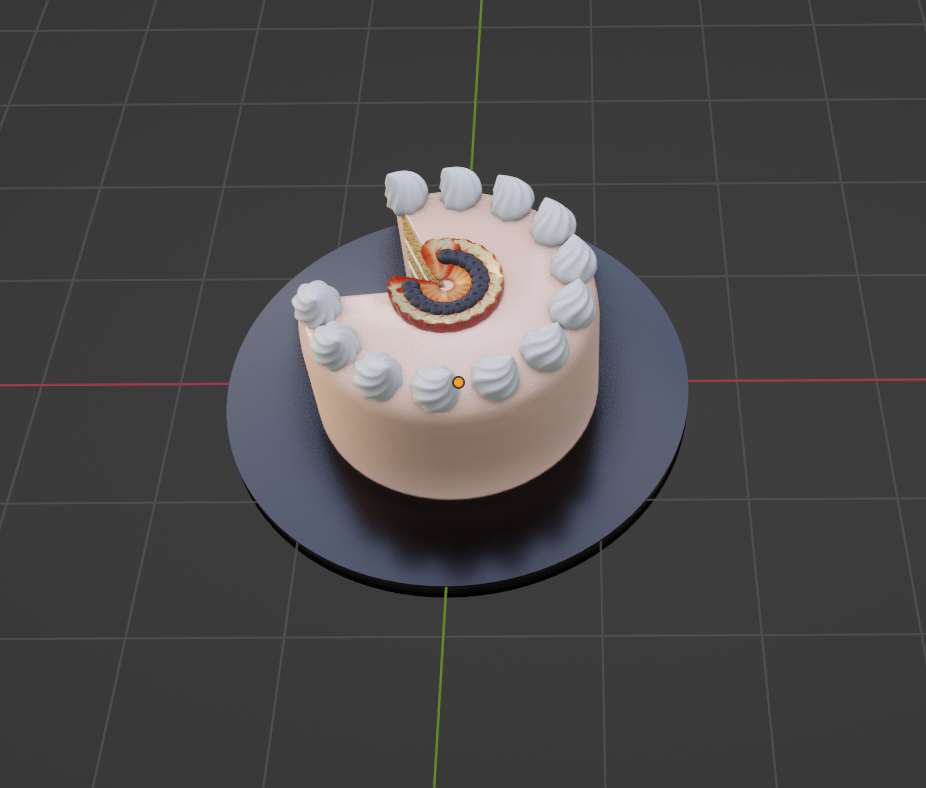
\includegraphics[scale=0.25]{./imgs/cakeParamMean/botSizeMin.png}
        \subcaption{CreamBot size 最小(0.0)}
 \end{minipage}
 \begin{minipage}[b]{0.48\linewidth}
  \centering
  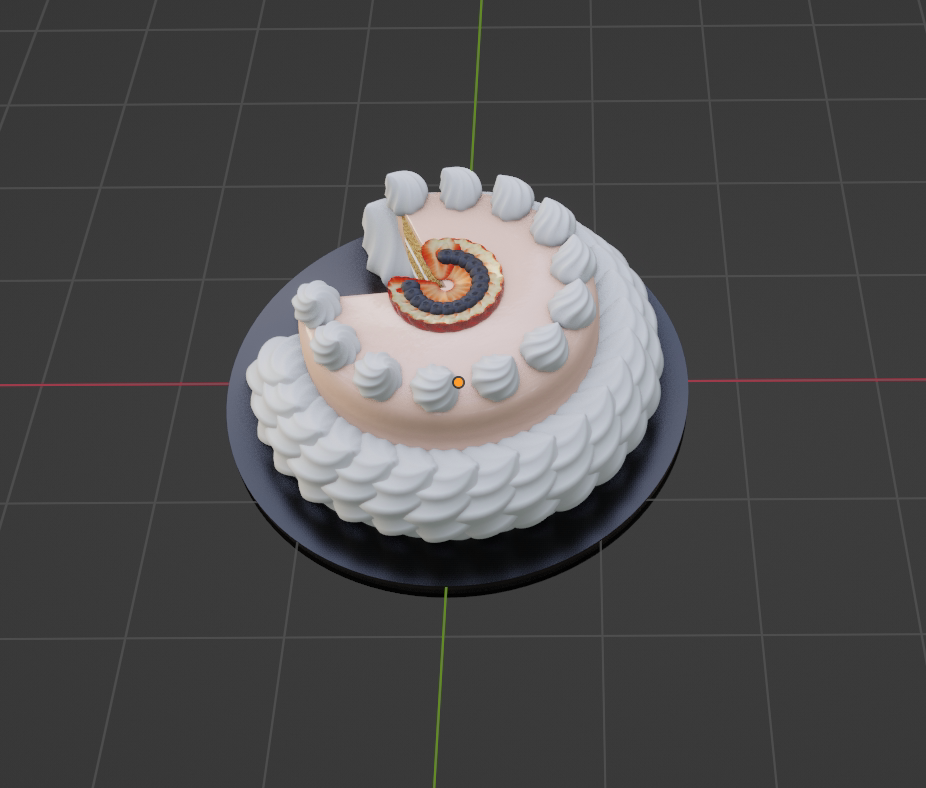
\includegraphics[scale=0.25]{./imgs/cakeParamMean/botSizeMax.png}
        \subcaption{CreamBot size 最大(2.0)}
 \end{minipage}\\
 \begin{minipage}[b]{0.48\linewidth}
  \centering
  \includegraphics[scale=0.25]{./imgs/cakeParamMean/topQuanMin.png}
        \subcaption{CreamTop quantity 最小(0.0)}
 \end{minipage}
 \begin{minipage}[b]{0.48\linewidth}
  \centering
  \includegraphics[scale=0.25]{./imgs/cakeParamMean/topQuanMax.png}
        \subcaption{CreamTop quantity 最大(50.0)}
 \end{minipage}
 \caption{Cake モデルにおけるパラメータ範囲(3)}\label{fig:cakeParamMean_3}
\end{figure}


\begin{figure}[h]
 \begin{minipage}[b]{0.48\linewidth}
  \centering
  \includegraphics[scale=0.25]{./imgs/cakeParamMean/topSizeMin.png}
        \subcaption{CreamTop size 最小(0.0)}
 \end{minipage}
 \begin{minipage}[b]{0.48\linewidth}
  \centering
  \includegraphics[scale=0.25]{./imgs/cakeParamMean/topSizeMax.png}
        \subcaption{CreamTop size 最大(2.0)}
 \end{minipage}\\
 \begin{minipage}[b]{0.48\linewidth}
  \centering
  \includegraphics[scale=0.25]{./imgs/cakeParamMean/plateSizeMin.png}
        \subcaption{Plate size 最小(0.3)}
 \end{minipage}
 \begin{minipage}[b]{0.48\linewidth}
  \centering
  \includegraphics[scale=0.25]{./imgs/cakeParamMean/plateSizeMax.png}
        \subcaption{Plate size 最大(1.0)}
 \end{minipage}\\
 \begin{minipage}[b]{0.48\linewidth}
  \centering
  \includegraphics[scale=0.25]{./imgs/cakeParamMean/tickMin.png}
        \subcaption{Plate thickness 最小(-0.2)}
 \end{minipage}
 \begin{minipage}[b]{0.48\linewidth}
  \centering
  \includegraphics[scale=0.25]{./imgs/cakeParamMean/tickMax.png}
        \subcaption{Plate thickness 最大(-0.1)}
 \end{minipage}
 \caption{Cake モデルにおけるパラメータ範囲(4)}\label{fig:cakeParamMean_4}
\end{figure}
\begin{figure}[h]
 \begin{minipage}[b]{0.48\linewidth}
  \centering
  \includegraphics[scale=0.17]{./imgs/sofaParamMean/depthMin.png}
        \subcaption{Depth 最小(0.2)}
 \end{minipage}
 \begin{minipage}[b]{0.48\linewidth}
  \centering
  \includegraphics[scale=0.17]{./imgs/sofaParamMean/depthMax.png}
        \subcaption{Depth 最大(4.0)}
 \end{minipage}\\
  \begin{minipage}[b]{0.48\linewidth}
  \centering
  \includegraphics[scale=0.17]{./imgs/sofaParamMean/widthMin.png}
        \subcaption{Width 最小(0.3)}
 \end{minipage}
 \begin{minipage}[b]{0.48\linewidth}
  \centering
  \includegraphics[scale=0.17]{./imgs/sofaParamMean/widthMax.png}
        \subcaption{Width 最大(5.0)}
 \end{minipage}\\
 \begin{minipage}[b]{0.48\linewidth}
  \centering
  \includegraphics[scale=0.17]{./imgs/sofaParamMean/legHeightMin.png}
        \subcaption{Legs height 最小(0.01)}
 \end{minipage}
 \begin{minipage}[b]{0.48\linewidth}
  \centering
  \includegraphics[scale=0.17]{./imgs/sofaParamMean/legHeightMax.png}
        \subcaption{Legs height 最大(1.0)}
 \end{minipage}\\
  \begin{minipage}[b]{0.48\linewidth}
  \centering
  \includegraphics[scale=0.17]{./imgs/sofaParamMean/legShapeMin.png}
        \subcaption{Leg shape 最小(0.0)}
 \end{minipage}
 \begin{minipage}[b]{0.48\linewidth}
  \centering
  \includegraphics[scale=0.17]{./imgs/sofaParamMean/legShapeMax.png}
        \subcaption{Leg shape 最大(20.0)}
 \end{minipage}
 \caption{Sofa モデルにおけるパラメータ範囲(1)}\label{fig:sofaParamMean_1}
\end{figure}


\begin{figure}[h]
 \begin{minipage}[b]{0.48\linewidth}
  \centering
  \includegraphics[scale=0.17]{./imgs/sofaParamMean/legDiameterMin.png}
        \subcaption{Leg diameter 最小(0.01)}
 \end{minipage}
 \begin{minipage}[b]{0.48\linewidth}
  \centering
  \includegraphics[scale=0.17]{./imgs/sofaParamMean/legDiameterMax.png}
        \subcaption{Leg diameter 最大(0.04)}
 \end{minipage}\\
 \begin{minipage}[b]{0.48\linewidth}
  \centering
  \includegraphics[scale=0.17]{./imgs/sofaParamMean/legAngleMin.png}
        \subcaption{Leg angle 最小(0.0)}
 \end{minipage}
 \begin{minipage}[b]{0.48\linewidth}
  \centering
  \includegraphics[scale=0.17]{./imgs/sofaParamMean/legAngleMax.png}
        \subcaption{Leg angle 最大(1.0)}
 \end{minipage}\\
  \begin{minipage}[b]{0.48\linewidth}
  \centering
  \includegraphics[scale=0.17]{./imgs/sofaParamMean/legPosMin.png}
        \subcaption{Leg position 最小(0.02)}
 \end{minipage}
 \begin{minipage}[b]{0.48\linewidth}
  \centering
  \includegraphics[scale=0.17]{./imgs/sofaParamMean/legPosMax.png}
        \subcaption{Leg position 最大(5.0)}
 \end{minipage}\\
 \begin{minipage}[b]{0.48\linewidth}
  \centering
  \includegraphics[scale=0.17]{./imgs/sofaParamMean/1BaseMin.png}
        \subcaption{Base height 最小(0.01)}
 \end{minipage}
 \begin{minipage}[b]{0.48\linewidth}
  \centering
  \includegraphics[scale=0.17]{./imgs/sofaParamMean/1BaseMax.png}
        \subcaption{Base height 最大(0.5)}
 \end{minipage}
 \caption{Sofa モデルにおけるパラメータ範囲(2)}\label{fig:sofaParamMean_2}
\end{figure}


\begin{figure}[h]
 \begin{minipage}[b]{0.48\linewidth}
  \centering
  \includegraphics[scale=0.17]{./imgs/sofaParamMean/Base2HeightMin.png}
        \subcaption{Base2 height 最小(0.01)}
 \end{minipage}
 \begin{minipage}[b]{0.48\linewidth}
  \centering
  \includegraphics[scale=0.17]{./imgs/sofaParamMean/Base2HeightMax.png}
        \subcaption{Base2 height 最大(0.5)}
 \end{minipage}\\
 \begin{minipage}[b]{0.48\linewidth}
  \centering
  \includegraphics[scale=0.17]{./imgs/sofaParamMean/backTickMin.png}
        \subcaption{Back thickness 最小(0.01)}
 \end{minipage}
 \begin{minipage}[b]{0.48\linewidth}
  \centering
  \includegraphics[scale=0.17]{./imgs/sofaParamMean/backTickMax.png}
        \subcaption{Back thickness 最大(0.3)}
 \end{minipage}\\
  \begin{minipage}[b]{0.48\linewidth}
  \centering
  \includegraphics[scale=0.17]{./imgs/sofaParamMean/backSideHeightMin.png}
        \subcaption{Back/Side height 最小(0.01)}
 \end{minipage}
 \begin{minipage}[b]{0.48\linewidth}
  \centering
  \includegraphics[scale=0.17]{./imgs/sofaParamMean/backSideHeightMax.png}
        \subcaption{Back/Side height 最大(1.5)}
 \end{minipage}\\
 \begin{minipage}[b]{0.48\linewidth}
  \centering
  \includegraphics[scale=0.17]{./imgs/sofaParamMean/sideNumMin.png}
        \subcaption{Side NO / 1 / YES 最小(0)}
 \end{minipage}
 \begin{minipage}[b]{0.48\linewidth}
  \centering
  \includegraphics[scale=0.17]{./imgs/sofaParamMean/sideNumMax.png}
        \subcaption{Side NO / 1 / YES 最大(2)}
 \end{minipage}
 \caption{Sofa モデルにおけるパラメータ範囲(3)}\label{fig:sofaParamMean_3}
\end{figure}


\begin{figure}[h]
 \begin{minipage}[b]{0.48\linewidth}
  \centering
  \includegraphics[scale=0.17]{./imgs/sofaParamMean/sideTicknessMin.png}
        \subcaption{Side thickness 最小(0.02)}
 \end{minipage}
 \begin{minipage}[b]{0.48\linewidth}
  \centering
  \includegraphics[scale=0.17]{./imgs/sofaParamMean/sideTicknessMax.png}
        \subcaption{Side thickness 最大(0.03)}
 \end{minipage}\\
 \begin{minipage}[b]{0.48\linewidth}
  \centering
  \includegraphics[scale=0.17]{./imgs/sofaParamMean/numCushionMin.png}
        \subcaption{N. of Cushions 最小(0)}
 \end{minipage}
 \begin{minipage}[b]{0.48\linewidth}
  \centering
  \includegraphics[scale=0.17]{./imgs/sofaParamMean/numCushionMax.png}
        \subcaption{N. of Cushions 最大(5)}
 \end{minipage}\\
  \begin{minipage}[b]{0.48\linewidth}
  \centering
  \includegraphics[scale=0.17]{./imgs/sofaParamMean/cushionTicknessMin.png}
        \subcaption{Cushion thickness 最小(0.05)}
 \end{minipage}
 \begin{minipage}[b]{0.48\linewidth}
  \centering
  \includegraphics[scale=0.17]{./imgs/sofaParamMean/cushionTicknessMax.png}
        \subcaption{Cushion thickness 最大(0.5)}
 \end{minipage}\\
 \begin{minipage}[b]{0.48\linewidth}
  \centering
  \includegraphics[scale=0.17]{./imgs/sofaParamMean/cushionNosingMin.png}
        \subcaption{Cushion nosing 最小(0.0)}
 \end{minipage}
 \begin{minipage}[b]{0.48\linewidth}
  \centering
  \includegraphics[scale=0.17]{./imgs/sofaParamMean/cushinoNosingMax.png}
        \subcaption{Cushion nosing 最大(0.3)}
 \end{minipage}
 \caption{Sofa モデルにおけるパラメータ範囲(4)}\label{fig:sofaParamMean_4}
\end{figure}


\begin{figure}[h]
 \begin{minipage}[b]{0.48\linewidth}
  \centering
  \includegraphics[scale=0.17]{./imgs/sofaParamMean/backCushionHeightMin.png}
        \subcaption{Back Cushion height 最小(0.1)}
 \end{minipage}
 \begin{minipage}[b]{0.48\linewidth}
  \centering
  \includegraphics[scale=0.17]{./imgs/sofaParamMean/backCushionHeightMax.png}
        \subcaption{Back Cushion height 最大(0.7)}
 \end{minipage}\\
 \begin{minipage}[b]{0.48\linewidth}
  \centering
  \includegraphics[scale=0.17]{./imgs/sofaParamMean/backCushionTickMin.png}
        \subcaption{Back Cush. Thickness / *Puffiness 最小(0.05)}
 \end{minipage}
 \begin{minipage}[b]{0.48\linewidth}
  \centering
  \includegraphics[scale=0.17]{./imgs/sofaParamMean/backCushionTickMax.png}
        \subcaption{Back Cush. Thickness / *Puffiness 最大(0.5)}
 \end{minipage}\\
  \begin{minipage}[b]{0.48\linewidth}
  \centering
  \includegraphics[scale=0.17]{./imgs/sofaParamMean/sideNumMin.png}
        \subcaption{Side Cushions NO / 1 / YES 最小(0)}
 \end{minipage}
 \begin{minipage}[b]{0.48\linewidth}
  \centering
  \includegraphics[scale=0.17]{./imgs/sofaParamMean/sideNumMax.png}
        \subcaption{Side Cushions NO / 1 / YES 最大(2)}
 \end{minipage}\\
 \begin{minipage}[b]{0.48\linewidth}
  \centering
  \includegraphics[scale=0.17]{./imgs/sofaParamMean/sideCushionHeightMin.png}
        \subcaption{Side Cushion Height 最小(0.1)}
 \end{minipage}
 \begin{minipage}[b]{0.48\linewidth}
  \centering
  \includegraphics[scale=0.17]{./imgs/sofaParamMean/sideCushionHeightMax.png}
        \subcaption{Side Cushion Height 最大(1.8)}
 \end{minipage}
 \caption{Sofa モデルにおけるパラメータ範囲(5)}\label{fig:sofaParamMean_5}
\end{figure}



\begin{figure}[h]
 \begin{minipage}[b]{0.48\linewidth}
  \centering
  \includegraphics[scale=0.17]{./imgs/sofaParamMean/sideCushionTickMin.png}
        \subcaption{Side Cushion Thickness 最小(0.0)}
 \end{minipage}
 \begin{minipage}[b]{0.48\linewidth}
  \centering
  \includegraphics[scale=0.17]{./imgs/sofaParamMean/sideCushionTickMax.png}
        \subcaption{Side Cushion Thickness 最大(0.05)}
 \end{minipage}\\
 \begin{minipage}[b]{0.48\linewidth}
  \centering
  \includegraphics[scale=0.17]{./imgs/sofaParamMean/stichingMin.png}
        \subcaption{Cushion Stitching 最小(0.0)}
 \end{minipage}
 \begin{minipage}[b]{0.48\linewidth}
  \centering
  \includegraphics[scale=0.17]{./imgs/sofaParamMean/stichingMax.png}
        \subcaption{Cushion Stitching 最大(0.05)}
 \end{minipage}\\
  \begin{minipage}[b]{0.48\linewidth}
  \centering
  \includegraphics[scale=0.17]{./imgs/sofaParamMean/creaseMin.png}
        \subcaption{Cushion Crease 最小(0.0)}
 \end{minipage}
 \begin{minipage}[b]{0.48\linewidth}
  \centering
  \includegraphics[scale=0.17]{./imgs/sofaParamMean/creaseMax.png}
        \subcaption{Cushion Crease 最大(0.3)}
 \end{minipage}\\
 \begin{minipage}[b]{0.48\linewidth}
  \centering
  \includegraphics[scale=0.17]{./imgs/sofaParamMean/bevelMin.png}
        \subcaption{Bevel 最小(0.001)}
 \end{minipage}
 \begin{minipage}[b]{0.48\linewidth}
  \centering
  \includegraphics[scale=0.17]{./imgs/sofaParamMean/bevelMax.png}
        \subcaption{Bevel 最大(1.0)}
 \end{minipage}
 \caption{Sofa モデルにおけるパラメータ範囲(6)}\label{fig:sofaParamMean_6}
\end{figure}



\begin{figure}[h]
 \begin{minipage}[b]{0.48\linewidth}
  \centering
  \includegraphics[scale=0.17]{./imgs/sofaParamMean/subdMin.png}
        \subcaption{Subd 最小(0)}
 \end{minipage}
 \begin{minipage}[b]{0.48\linewidth}
  \centering
  \includegraphics[scale=0.17]{./imgs/sofaParamMean/subdMax.png}
        \subcaption{Subd 最大(2)}
 \end{minipage}
 \caption{Sofa モデルにおけるパラメータ範囲(7)}\label{fig:sofaParamMean_7}
\end{figure}

\clearpage

\setcounter{table}{0}
\setcounter{figure}{0}

\section{提案モデルの推移}\label{appendix:gaChange}
本付録では,遺伝的アルゴリズムの推移を具体的なグラフを用いて示す.
図\ref{fig:gaChange1_1} - \ref{fig:gaChange1_3}に
実験1における具体的な提案モデルの推移を,
図\ref{fig:gaChange2_1} - \ref{fig:gaChange2_3}に
実験2における具体的な提案モデルの推移を示す.
既存の研究では縦軸は適応度が利用されるが,本研究では選択によって行われるため実験1では見本モデルとの,実験2では最後に作成されたモデルとのユークリッド距離を用いる.この時,各遺伝子の定義域について Min - Max normalization を事前処理として行っている.また,箱ひげ図が各ステップの提案モデル群,折れ線グラフが次ステップに進む前に決定されたモデルを意味する.

\begin{figure}[h]
 \begin{minipage}[b]{0.48\linewidth}
  \centering
  \includegraphics[scale=0.15]{./imgs/gaChange/cake1_1.pdf}
        \subcaption{被験者1,提案システム}
 \end{minipage}
 \begin{minipage}[b]{0.48\linewidth}
  \centering
  \includegraphics[scale=0.15]{./imgs/gaChange/cake2_1.pdf}
        \subcaption{被験者1,既存システム}
 \end{minipage}\\
 \begin{minipage}[b]{0.48\linewidth}
  \centering
  \includegraphics[scale=0.15]{./imgs/gaChange/cake1_2.pdf}
        \subcaption{被験者2,提案システム}
 \end{minipage}
 \begin{minipage}[b]{0.48\linewidth}
  \centering
  \includegraphics[scale=0.15]{./imgs/gaChange/cake2_2.pdf}
        \subcaption{被験者2,既存システム}
 \end{minipage}\\
 \begin{minipage}[b]{0.48\linewidth}
  \centering
  \includegraphics[scale=0.15]{./imgs/gaChange/cake1_3.pdf}
        \subcaption{被験者3,提案システム}
 \end{minipage}
 \begin{minipage}[b]{0.48\linewidth}
  \centering
  \includegraphics[scale=0.15]{./imgs/gaChange/cake2_3.pdf}
        \subcaption{被験者3,既存システム}
 \end{minipage}\\
 \begin{minipage}[b]{0.48\linewidth}
  \centering
  \includegraphics[scale=0.15]{./imgs/gaChange/cake1_4.pdf}
        \subcaption{被験者4,提案システム}
 \end{minipage}
 \begin{minipage}[b]{0.48\linewidth}
  \centering
  \includegraphics[scale=0.15]{./imgs/gaChange/cake2_4.pdf}
        \subcaption{被験者4,既存システム}
 \end{minipage}
 \caption{実験1における提案モデルの推移(1)}\label{fig:gaChange1_1}
\end{figure}

\begin{figure}[h]
 \begin{minipage}[b]{0.48\linewidth}
  \centering
  \includegraphics[scale=0.15]{./imgs/gaChange/cake1_5.pdf}
        \subcaption{被験者5,提案システム}
 \end{minipage}
 \begin{minipage}[b]{0.48\linewidth}
  \centering
  \includegraphics[scale=0.15]{./imgs/gaChange/cake2_5.pdf}
        \subcaption{被験者5,既存システム}
 \end{minipage}\\
 \begin{minipage}[b]{0.48\linewidth}
  \centering
  \includegraphics[scale=0.15]{./imgs/gaChange/cake1_6.pdf}
        \subcaption{被験者6,提案システム}
 \end{minipage}
 \begin{minipage}[b]{0.48\linewidth}
  \centering
  \includegraphics[scale=0.15]{./imgs/gaChange/cake2_6.pdf}
        \subcaption{被験者6,既存システム}
 \end{minipage}\\
 \begin{minipage}[b]{0.48\linewidth}
  \centering
  \includegraphics[scale=0.15]{./imgs/gaChange/cake1_7.pdf}
        \subcaption{被験者7,提案システム}
 \end{minipage}
 \begin{minipage}[b]{0.48\linewidth}
  \centering
  \includegraphics[scale=0.15]{./imgs/gaChange/cake2_7.pdf}
        \subcaption{被験者7,既存システム}
 \end{minipage}\\
 \begin{minipage}[b]{0.48\linewidth}
  \centering
  \includegraphics[scale=0.15]{./imgs/gaChange/cake1_8.pdf}
        \subcaption{被験者8,提案システム}
 \end{minipage}
 \begin{minipage}[b]{0.48\linewidth}
  \centering
  \includegraphics[scale=0.15]{./imgs/gaChange/cake2_8.pdf}
        \subcaption{被験者8,既存システム}
 \end{minipage}
 \caption{実験1における提案モデルの推移(2)}\label{fig:gaChange1_2}
\end{figure}

\begin{figure}[h]
 \begin{minipage}[b]{0.48\linewidth}
  \centering
  \includegraphics[scale=0.15]{./imgs/gaChange/cake1_9.pdf}
        \subcaption{被験者9,提案システム}
 \end{minipage}
 \begin{minipage}[b]{0.48\linewidth}
  \centering
  \includegraphics[scale=0.15]{./imgs/gaChange/cake2_9.pdf}
        \subcaption{被験者9,既存システム}
 \end{minipage}\\
 \begin{minipage}[b]{0.48\linewidth}
  \centering
  \includegraphics[scale=0.15]{./imgs/gaChange/cake1_10.pdf}
        \subcaption{被験者10,提案システム}
 \end{minipage}
 \begin{minipage}[b]{0.48\linewidth}
  \centering
  \includegraphics[scale=0.15]{./imgs/gaChange/cake2_10.pdf}
        \subcaption{被験者10,既存システム}
 \end{minipage}\\
 \begin{minipage}[b]{0.48\linewidth}
  \centering
  \includegraphics[scale=0.15]{./imgs/gaChange/cake1_11.pdf}
        \subcaption{被験者11,提案システム}
 \end{minipage}
 \begin{minipage}[b]{0.48\linewidth}
  \centering
  \includegraphics[scale=0.15]{./imgs/gaChange/cake2_11.pdf}
        \subcaption{被験者11,既存システム}
 \end{minipage}
 \caption{実験1における提案モデルの推移(3)}\label{fig:gaChange1_3}
\end{figure}

\begin{figure}[h]
 \begin{minipage}[b]{0.48\linewidth}
  \centering
  \includegraphics[scale=0.15]{./imgs/gaChange/sofa1_1.pdf}
        \subcaption{被験者1,提案システム}
 \end{minipage}
 \begin{minipage}[b]{0.48\linewidth}
  \centering
  \includegraphics[scale=0.15]{./imgs/gaChange/sofa2_1.pdf}
        \subcaption{被験者1,既存システム}
 \end{minipage}\\
 \begin{minipage}[b]{0.48\linewidth}
  \centering
  \includegraphics[scale=0.15]{./imgs/gaChange/sofa1_2.pdf}
        \subcaption{被験者2,提案システム}
 \end{minipage}
 \begin{minipage}[b]{0.48\linewidth}
  \centering
  \includegraphics[scale=0.15]{./imgs/gaChange/sofa2_2.pdf}
        \subcaption{被験者2,既存システム}
 \end{minipage}\\
 \begin{minipage}[b]{0.48\linewidth}
  \centering
  \includegraphics[scale=0.15]{./imgs/gaChange/sofa1_3.pdf}
        \subcaption{被験者3,提案システム}
 \end{minipage}
 \begin{minipage}[b]{0.48\linewidth}
  \centering
  \includegraphics[scale=0.15]{./imgs/gaChange/sofa2_3.pdf}
        \subcaption{被験者3,既存システム}
 \end{minipage}\\
 \begin{minipage}[b]{0.48\linewidth}
  \centering
  \includegraphics[scale=0.15]{./imgs/gaChange/sofa1_4.pdf}
        \subcaption{被験者4,提案システム}
 \end{minipage}
 \begin{minipage}[b]{0.48\linewidth}
  \centering
  \includegraphics[scale=0.15]{./imgs/gaChange/sofa2_4.pdf}
        \subcaption{被験者4,既存システム}
 \end{minipage}
 \caption{実験2における提案モデルの推移(1)}\label{fig:gaChange2_1}
\end{figure}

\begin{figure}[h]
 \begin{minipage}[b]{0.48\linewidth}
  \centering
  \includegraphics[scale=0.15]{./imgs/gaChange/sofa1_5.pdf}
        \subcaption{被験者5,提案システム}
 \end{minipage}
 \begin{minipage}[b]{0.48\linewidth}
  \centering
  \includegraphics[scale=0.15]{./imgs/gaChange/sofa2_5.pdf}
        \subcaption{被験者5,既存システム}
 \end{minipage}\\
 \begin{minipage}[b]{0.48\linewidth}
  \centering
  \includegraphics[scale=0.15]{./imgs/gaChange/sofa1_6.pdf}
        \subcaption{被験者6,提案システム}
 \end{minipage}
 \begin{minipage}[b]{0.48\linewidth}
  \centering
  \includegraphics[scale=0.15]{./imgs/gaChange/sofa2_6.pdf}
        \subcaption{被験者6,既存システム}
 \end{minipage}\\
 \begin{minipage}[b]{0.48\linewidth}
  \centering
  \includegraphics[scale=0.15]{./imgs/gaChange/sofa1_7.pdf}
        \subcaption{被験者7,提案システム}
 \end{minipage}
 \begin{minipage}[b]{0.48\linewidth}
  \centering
  \includegraphics[scale=0.15]{./imgs/gaChange/sofa2_7.pdf}
        \subcaption{被験者7,既存システム}
 \end{minipage}\\
 \begin{minipage}[b]{0.48\linewidth}
  \centering
  \includegraphics[scale=0.15]{./imgs/gaChange/sofa1_8.pdf}
        \subcaption{被験者8,提案システム}
 \end{minipage}
 \begin{minipage}[b]{0.48\linewidth}
  \centering
  \includegraphics[scale=0.15]{./imgs/gaChange/sofa2_8.pdf}
        \subcaption{被験者8,既存システム}
 \end{minipage}
 \caption{実験2における提案モデルの推移(2)}\label{fig:gaChange2_2}
\end{figure}

\begin{figure}[h]
 \begin{minipage}[b]{0.48\linewidth}
  \centering
  \includegraphics[scale=0.15]{./imgs/gaChange/sofa1_9.pdf}
        \subcaption{被験者9,提案システム}
 \end{minipage}
 \begin{minipage}[b]{0.48\linewidth}
  \centering
  \includegraphics[scale=0.15]{./imgs/gaChange/sofa2_9.pdf}
        \subcaption{被験者9,既存システム}
 \end{minipage}\\
 \begin{minipage}[b]{0.48\linewidth}
  \centering
  \includegraphics[scale=0.15]{./imgs/gaChange/sofa1_10.pdf}
        \subcaption{被験者10,提案システム}
 \end{minipage}
 \begin{minipage}[b]{0.48\linewidth}
  \centering
  \includegraphics[scale=0.15]{./imgs/gaChange/sofa2_10.pdf}
        \subcaption{被験者10,既存システム}
 \end{minipage}\\
 \begin{minipage}[b]{0.48\linewidth}
  \centering
  \includegraphics[scale=0.15]{./imgs/gaChange/sofa1_11.pdf}
        \subcaption{被験者11,提案システム}
 \end{minipage}
 \begin{minipage}[b]{0.48\linewidth}
  \centering
  \includegraphics[scale=0.15]{./imgs/gaChange/sofa2_11.pdf}
        \subcaption{被験者11,既存システム}
 \end{minipage}
 \caption{実験3における提案モデルの推移(3)}\label{fig:gaChange2_3}
\end{figure}

\clearpage

\setcounter{table}{0}
\setcounter{figure}{0}

\section{提案モデルパラメータの二次元可視化}\label{appendix:tSNE}
\hyperref[appendix:gaChange]{付録B}で示した提案モデルの推移では,提案モデルパラメータを最終モデルとの距離によって視覚化したが、それだけでは探索範囲の比較が難しい.そこで本章では t-SNE \cite{van2008visualizing} という手法により二次元に次元削減を行う.
図\ref{fig:tSNE1_1},\ref{fig:tSNE1_2}に実験1を,図\ref{fig:tSNE2_1},\ref{fig:tSNE2_2}に実験2の結果を示す.
この散布図について縁取りが青いものが提案システム,赤いものが既存システムによる提案モデルであり,内部の色が0から1に行くにつれてステップ数が増加するようにしている. また,軸についてはそれぞれ無次元量である.

\begin{figure}[h]
 \begin{minipage}[b]{0.48\linewidth}
  \centering
  \includegraphics[scale=0.15]{./imgs/tSNE/cake_1.pdf}
        \subcaption{被験者1}
 \end{minipage}
 \begin{minipage}[b]{0.48\linewidth}
  \centering
  \includegraphics[scale=0.15]{./imgs/tSNE/cake_2.pdf}
        \subcaption{被験者2}
 \end{minipage}\\
 \begin{minipage}[b]{0.48\linewidth}
  \centering
  \includegraphics[scale=0.15]{./imgs/tSNE/cake_3.pdf}
        \subcaption{被験者3}
 \end{minipage}
 \begin{minipage}[b]{0.48\linewidth}
  \centering
  \includegraphics[scale=0.15]{./imgs/tSNE/cake_4.pdf}
        \subcaption{被験者4}
 \end{minipage}\\
 \begin{minipage}[b]{0.48\linewidth}
  \centering
  \includegraphics[scale=0.15]{./imgs/tSNE/cake_5.pdf}
        \subcaption{被験者5}
 \end{minipage}
 \begin{minipage}[b]{0.48\linewidth}
  \centering
  \includegraphics[scale=0.15]{./imgs/tSNE/cake_6.pdf}
        \subcaption{被験者6}
 \end{minipage}\\
 \caption{実験1におけるパラメータの二次元可視化(1)}\label{fig:tSNE1_1}
\end{figure}

\begin{figure}[h]
 \begin{minipage}[b]{0.48\linewidth}
  \centering
  \includegraphics[scale=0.15]{./imgs/tSNE/cake_7.pdf}
        \subcaption{被験者7}
 \end{minipage}
 \begin{minipage}[b]{0.48\linewidth}
  \centering
  \includegraphics[scale=0.15]{./imgs/tSNE/cake_8.pdf}
        \subcaption{被験者8}
 \end{minipage}\\
 \begin{minipage}[b]{0.48\linewidth}
  \centering
  \includegraphics[scale=0.15]{./imgs/tSNE/cake_9.pdf}
        \subcaption{被験者9}
 \end{minipage}
 \begin{minipage}[b]{0.48\linewidth}
  \centering
  \includegraphics[scale=0.15]{./imgs/tSNE/cake_10.pdf}
        \subcaption{被験者10}
 \end{minipage}\\
 \begin{minipage}[b]{0.48\linewidth}
  \centering
  \includegraphics[scale=0.15]{./imgs/tSNE/cake_11.pdf}
        \subcaption{被験者11}
 \end{minipage}\\
 \caption{実験1におけるパラメータの二次元可視化(2)}\label{fig:tSNE1_2}
\end{figure}



\begin{figure}[h]
 \begin{minipage}[b]{0.48\linewidth}
  \centering
  \includegraphics[scale=0.15]{./imgs/tSNE/sofa_1.pdf}
        \subcaption{被験者1}
 \end{minipage}
 \begin{minipage}[b]{0.48\linewidth}
  \centering
  \includegraphics[scale=0.15]{./imgs/tSNE/sofa_2.pdf}
        \subcaption{被験者2}
 \end{minipage}\\
 \begin{minipage}[b]{0.48\linewidth}
  \centering
  \includegraphics[scale=0.15]{./imgs/tSNE/sofa_3.pdf}
        \subcaption{被験者3}
 \end{minipage}
 \begin{minipage}[b]{0.48\linewidth}
  \centering
  \includegraphics[scale=0.15]{./imgs/tSNE/sofa_4.pdf}
        \subcaption{被験者4}
 \end{minipage}\\
 \begin{minipage}[b]{0.48\linewidth}
  \centering
  \includegraphics[scale=0.15]{./imgs/tSNE/sofa_5.pdf}
        \subcaption{被験者5}
 \end{minipage}
 \begin{minipage}[b]{0.48\linewidth}
  \centering
  \includegraphics[scale=0.15]{./imgs/tSNE/sofa_6.pdf}
        \subcaption{被験者6}
 \end{minipage}\\
 \caption{実験2におけるパラメータの二次元可視化(1)}\label{fig:tSNE2_1}
\end{figure}

\begin{figure}[h]
 \begin{minipage}[b]{0.48\linewidth}
  \centering
  \includegraphics[scale=0.15]{./imgs/tSNE/sofa_7.pdf}
        \subcaption{被験者7}
 \end{minipage}
 \begin{minipage}[b]{0.48\linewidth}
  \centering
  \includegraphics[scale=0.15]{./imgs/tSNE/sofa_8.pdf}
        \subcaption{被験者8}
 \end{minipage}\\
 \begin{minipage}[b]{0.48\linewidth}
  \centering
  \includegraphics[scale=0.15]{./imgs/tSNE/sofa_9.pdf}
        \subcaption{被験者9}
 \end{minipage}
 \begin{minipage}[b]{0.48\linewidth}
  \centering
  \includegraphics[scale=0.15]{./imgs/tSNE/sofa_10.pdf}
        \subcaption{被験者10}
 \end{minipage}\\
 \begin{minipage}[b]{0.48\linewidth}
  \centering
  \includegraphics[scale=0.15]{./imgs/tSNE/sofa_11.pdf}
        \subcaption{被験者11}
 \end{minipage}\\
 \caption{実験2におけるパラメータの二次元可視化(2)}\label{fig:tSNE2_2}
\end{figure}

\end{document}
